\documentclass[a4paper]{article}

% Language and font encodings
\usepackage[english]{babel}
\usepackage[T1]{fontenc}

% Sets page size and margins
\usepackage[a4paper,top=3cm,bottom=2cm,left=3cm,right=3cm,marginparwidth=1.75cm]{geometry}

% Useful packages
\usepackage{amsmath}
\usepackage{graphicx}
\usepackage[colorinlistoftodos]{todonotes}
\usepackage[colorlinks=true, allcolors=black]{hyperref}
\usepackage{parskip}
\usepackage{float}

\usepackage{booktabs}
\usepackage{tabularx}
\usepackage{amssymb} 

% APA-style references
\usepackage{csquotes}
\usepackage[style=apa,backend=biber,natbib=true]{biblatex}
\addbibresource{sample.bib}


\newcommand{\ganttbar}{\rule{1.2em}{0.7ex}}
\newcommand{\milestone}{\raisebox{0.1ex}{\ensuremath{\blacklozenge}}}

\begin{document}
\thispagestyle{empty}

\vspace*{\fill}
\begin{center}

{\Huge\bfseries Featback Meets AI\par}

\vspace{0.8em}
{\LARGE Assignment Phase 2 -- Group EADS G\par}

\vspace{1.5em}
{\large Sara De Marchi (s.de.marchi@student.tue.nl),\\
Seeam Amini (s.amini@student.tue.nl),\\
Ritik Ghanshani (r.s.ghanshani@student.tue.nl),\\
Nikhil Kamath (n.s.kamath@student.tue.nl).\par}

\today
\end{center}
\vspace*{\fill}

\newpage

\tableofcontents

\vspace{3.5em}
\subsection*{Word count per section}
\begin{tabularx}{\textwidth}{@{}Xrr@{}}
\toprule
Section & Words & Limit \\
\midrule
1 Public Summary & 150 & 150 \\
2 Comprehensive Summary & 2,836 & 2,000 \\
3 Responsible Innovation Project Statement & 987 & 1,000 \\
4 User Narrative & 377 & 500 \\
5 Visual Representation of the Mock-up & 1 page & 1 A4 page \\
6 Documentation (incl.\ prompts and code) & 1,662 & - \\
\bottomrule
\end{tabularx}

\smallskip
\small Counted on the compiled text of each section: headings, figure text, references and page numbers excluded; in-text citations included.
\normalsize

\newpage

\section{Public Summary} % Max 150 words, simple language.
% Questions addressed and tool created; importance for stakeholders/public; expected challenges.
Many people with eating-disorder symptoms wait years before getting help. Featback is a free, anonymous online program that sends users a weekly feedback message after four questions. Every message is picked from a pre-approved bank, so it often misses what the person went through, and many users stop using the program early.

This project asks whether AI can make these messages more personal while keeping them safe. Our mock-up adds an optional fifth open question. AI writes only the personal parts of the message, using what the user wrote, while the expert-written advice stays unchanged. Any sign of serious danger, such as self-harm, triggers a fixed message pointing to professional help.

A fitting message may help users feel heard, keep using the program and be supported on the way to care. The main challenges are spotting danger reliably, fairness to people who write little, privacy, and knowing whether personalization helps.

\newpage

\section{Comprehensive Summary} % Max 2000 words in total.

\subsection{Problem Definition and Objectives} 
% The problem, the change we want to achieve, and whose problem it is.
Featback is a low-threshold program that reaches people with eating-disorder symptoms before they enter care. According to the client, its main goal is awareness and help-seeking, followed by symptom reduction. 

Each week, users answer four questions on weight and shape concerns, nutrition and dieting, binge eating and compensatory behaviors, with four answer options each. The weekly feedback message is chosen from a bank of about 1,250 pre-written messages, according to whether each answer is in the healthy or unhealthy range and whether it improved \citep{rohrbach2022featback, rohrbach2019protocol}. Two kinds of information never reach the message. One is change within an answer option: three binge days one week and one the next both read ``1--3 days''. The other is anything the questions do not ask about, such as a stressful exam week.

The client finds the message too rigid and names retention as the central weakness, since many visitors try Featback and do not stay. She treats feeling heard as the main quality measure, suggests that users in danger are only pointed to help, and names relief of waiting lists as a goal. Three groups share the problem. Users are anonymous, untreated people who find it harder to feel heard and to come back when the message ignores their experience. The client and its clinicians want users to stay long enough to seek help. The care system gains early detection. Our tool cannot shorten waiting lists, and more people seeking help could even lengthen them; it can keep people supported while they wait.

Delays in reaching care are long across the care system. In help-seeking samples, untreated eating disorder lasts on average 29.9 months for anorexia nervosa, 53.0 for bulimia nervosa and 67.4 for binge eating disorder, and shortening it may improve outcomes \citep{austin2021duration}. In the Netherlands it often takes more than four years to seek treatment \citep{rohrbach2019protocol}, as the client also told us.

Personalization means tailoring the message to the individual's own symptoms and stated experience. Retention is the number of weekly check-ins completed in the eight-week program (0--8), as in the Featback trials \citep{rohrbach2019protocol}. Acute risk means any sign that the user may be in danger now, such as suicidal thoughts or self-harm.

The change we want is a weekly message that reflects what the user reported and is safe to send without clinician review. Our objectives are to:
\begin{enumerate}
  \item personalize two parts of the message, a summary with one line of empathy that reflects what the user reported and a short encouraging closing, using the four answers, the optional fifth question and, where available, earlier weeks;
  \item keep the psychoeducation and the tips expert-written and pre-approved;
  \item handle acute-risk input without AI generation, with a fixed reply pointing to professional help;
  \item tell users that AI is involved, and keep the fifth question optional, with consent given once and withdrawable;
  \item build and evaluate a mock-up on synthetic data and check the design against the Belmont principles.
\end{enumerate}
The mock-up shows that the pipeline works on synthetic inputs (Section \ref{subsection 2.3}). It is not clinically validated and cannot show that personalization improves retention, which needs a trial with real users, so we treat that benefit as a hypothesis.

\subsection{Background: Current Approaches and Knowledge} 

A randomized trial with 355 participants, 43\% of whom had never received eating-disorder treatment, compared Featback, expert-patient support by chat or e-mail, and the two combined against a waiting list \citep{rohrbach2022featback}. All three reduced symptoms more than the waiting list, with no difference among them. Featback alone scored lower on satisfaction (5.8 out of 10, against 7.1 and 7.4 with expert-patient support), and 84.1\% of its participants completed at least five of eight weekly check-ins. Joining a trial differs from visiting the public website, where the client reports that many visitors do not stay. Featback is thus already tailored to the four answers; our work goes further by using what the user writes.

Personalization is widely assumed to drive engagement, but the evidence is scarce. Among 138 studies of digital interventions for depression, \citet{hornstein2023personalization} found only two direct comparisons of a more and a less personalized version, both with small samples. \citet{matthews2025personalisation} reach a similar conclusion for mental health apps in general. For the open question, \citet{arditi2020computer} found that free-text comments in a cancer patient survey held personal and emotional themes that the closed questions missed.

\citet{fardouly2022ml} review machine learning for eating disorders. They call for more work on how chatbots handle unanticipated input, and warn that most models were built on data from young white women and may not generalize. \citet{monaco2024advanced} propose a similar platform for Italy, without outcome data yet.

Featback's existing safety handling is rule-based. In the trial, a BMI of 15 or lower, or compensatory behavior or bingeing every day for a week, triggered an alarm to the researcher and an e-mail recommending professional help. Expert patients referred suicidal ideation to Stichting 113, a Dutch suicide prevention service \citep{rohrbach2019protocol}. Our design assumes no reviewer and notifies nobody at Featback, in line with the client's suggestion to point users to help only. A word-list check and an AI check read the free text added by the fifth question before any feedback message is written (Section \ref{subsection 2.3}).

General-purpose chatbots handle risk poorly. \citet{heston2023safety} found that mental health chatbots delayed referral to a human to potentially dangerous levels, and \citet{clark2025ability} found that AI therapy and companion bots endorsed harmful proposals from distressed fictional adolescents in 19 of 60 opportunities. \citet{lawrence2024opportunities} call this a structural risk of large language models, and \citet{BOLPAGNI2026101043} ground safer design in triage and stepped care. Hence acute input never reaches the writing model, and generation is confined to the personal parts of the message.

Taken together, we found no study combining AI-written, personalized messages in an anonymous, low-threshold self-help program for eating disorders, with expert-written content at the core and no clinician reviewing the output. This combination is the gap our mock-up addresses.

\subsection{Plan of Approach and Design Strategy} \label{subsection 2.3}

Our plan updates one thing in the user's week: the message they get back after the check-in. Today a message is picked from a bank of 1,250 expert-written messages and sent as it is. In our design it is still picked from the bank, but personalized parts are written around it. We add an optional, open-ended fifth question that invites the user to share something about their week, and we also use the data from previous weeks, so that the part describing the user's week responds to the week they actually reported. The intended impact: users feel heard, stay with the weekly cadence, and are carried further toward help. For the client, this is retention in a tool whose only job is to keep people engaged and supported while they wait for care. We design against the Belmont principles of respect for persons, beneficence and justice, using Design for Values as our method, so every choice below answers to a named value.

The week is handled in four moves, and the first is safety. The fifth answer is checked in two layers before the AI writer sees it. The first is word recognition: the text is matched against English and Dutch lists of acute, sensitive and on-topic wording. On topic means eating, food, the body and the person's own feelings; anything else, such as the app, money, housing, news, sport or weather, is off-topic and gets one fixed line restating that limit instead of a personal part. The acute list follows the categories of the Columbia Suicide Severity Rating Scale \citep{posner2011} and uses the wording of its Dutch translation. If it says acute, the process stops and the text never reaches the next layer. The second is an AI check: a classifier answers with exactly one word (acute, sensitive, off-topic or routine) and cannot write a message. Either layer alone can stop a message; when they disagree, the more severe answer wins, and if the AI check fails, the word list is trusted. This is triage and stepped care in miniature: risk first, then a matched response. For an acute answer nothing is generated. The user gets a fixed message pointing to 113, the Proud2Bme chat and the Eetstoornissennetwerk care finder, which notes that the other answers were saved; no one at Featback is notified, since the client suggested pointing to help only. Sensitive answers currently receive the regular message.

Second, selection. The selector embeds the bank once and stores the vectors in a file. In our mock-up the bank is synthetic, generated for this assignment; in practice it would hold the expert-written messages. Each week the selector matches the week's answers against the bank and returns the closest message, after a label filter removes messages written for a completely opposite week, for example one for someone who is improving when the answers report worse binges. Selection needs no language model and is deterministic.

Third, the writer. Whenever a user answers Question 5, the fine-tuned model produces two personal components that are added to the selected base message: a summary that opens with one line of empathy and echoes back what the user reported, and a short closing that encourages without giving new advice. We also use the data from previous weeks to mention trends, with empathy and care. Nothing clinical is written; the psychoeducation and the tips arrive with the selected message. Off-topic weeks get one line reinforcing the boundary instead.

Fourth, the post-check. Before anything is sent, a script drops anything copied from the bank or repeated from the person's answer, and rejects the personal part if it contains digits or weight and calorie units, names a condition, or does not pick up the user's own words. It is deliberately narrow, which we return to in the challenges.

Each choice has a reason. The bank stays because the psychoeducation and the tips should remain expert-written and pre-approved. The fine-tune is needed because the tone must match Featback's existing messages reliably. The model is small and local because the proof of concept has to run on student resources, which also means real user data does not move anywhere. Every message states that AI was involved in writing it, and the fifth question is optional, with consent given once and withdrawable.

The mock-up runs entirely on synthetic material built to carry the structure of the real system. The core data set has one synthetic answer for each of the 256 answer combinations of the four questions, so every combination appears exactly once; 231 are used for training and 25 are held out as test data. The model's input is the week's four answers written out in words, using the questionnaire's labels (the model reads text, and the words carry both the level and the direction of the change), plus the base message the selector picked. The expected output is only the two personal components. The fine-tune is a small open model (Qwen3.5-4B) trained with a LoRA adapter for 120 optimizer steps on one consumer GPU. On the 25 held-out combinations we check mechanically whether the model echoes the severity wording the user reported and whether it ends after the closing. The fine-tuned model met both checks in all 25 cases; the untuned base model managed 4 of 25 on severity wording and ran on in every case. The bank holds the expert content, the psychoeducation and the tips; the client reviews it for equivalence in structure and tone, our stand-in for the real bank she did not share.

We evaluate three parts of the system: the safety pass (detection rate and false alarms), the selector (accuracy), and the full pipeline (four rubric scores). The safety pass is tested at sentence level on 220 sentences written by AI agents that never saw the code. Each carries a label (acute, sensitive, off-topic or routine) from the start, which a script compares with the gate's answer. The first set of 105 (34 acute, 71 others) was used to build the word list and the AI prompt; the second, of 115 (35 acute, 80 others), was kept back for a fair test. On the first set the word list found 32 of the 34 acute sentences without a false alarm, but on the second only 9 of 35, with 3 false alarms among the 80 others, so the AI check carries most of the load. That check found all 34 acute sentences of the first set, with 8 false alarms among the 71 others, and has not been run on the second set yet. The selector has a held-out check of its own: for each held-out week the correct message is the bank entry written for that answer combination, and accuracy is the share of weeks where the selector returns it. The label is a filter, not a threshold; the embedding ranks what remains. Finally, the full pipeline runs ten synthetic weekly check-ins covering all four tracks, and the client and clinicians score each message from 0 to 10 on structure, tone, tip fit and safety, against a written rubric that gives every rater the same descriptors. The client's example message is scored first, blind, as a fixed reference. A message passes if it has four components, no diagnosis, a tone that matches the example, a tip that fits what was reported and, for an acute answer, a reply from the approved resource set. A personal part of more than eight sentences counts as a loop and is dropped. The mock-up shows the pipeline works on synthetic inputs; it is not clinically validated, the training material is ours rather than the client's, and it does not replace professional judgment.

Realizing the potential of this addition requires specific actions from the people around Featback. The client has to supply the real bank of expert-written messages, and the clinicians have to approve the acute reply wording and score the mock-up's outputs. The mock-up also has three key challenges to address before deployment. The first is detection of acute responses. The word list cannot adapt to new phrasings, so the AI check carries most of the load, yet it was tuned and tested on the same data it is later judged against. Its false alarms show that a past low point or a song quote can be read as crisis, and the consequences of an error are not symmetric: a false alarm means no personalized message, while a miss can have far more serious consequences. The second is equity: open-ended text favors users who write well. Everyone gets a response, even to a two-word answer, but the personal part can only reflect what the user gives the model. The third is retention from personalization, which is a hypothesis for now; testing it needs a trial with real users.

\subsection{Comparison to Alternatives}

Our Phase 1's second design, which was prompting only (Design B), had the model write the entire message from a prompt carrying the published example message and five or six worked examples, with no bank and no training. Its main benefit is that it is the cheapest way to make every sentence respond to the fifth question. We set it aside because it discards the bank, and with the bank goes the guarantee that the clinical content is expert-written and pre-approved. Every message would be self-generated, including the psychoeducation and the tips a clinician signs off on today, with no clinician in the loop; that is the weakest position on beneficence.

Outside the project, the alternatives fall into three shapes. The closest is human support: Featback's own trial paired the program with expert-patient chat and email, which matched the automated program on symptoms but scored higher on satisfaction (7.1 and 7.4 against 5.8, Section~2.2); a person writing each reply is the part that does not scale. At the other end, chatbots answer in open conversation. Therabot, the first generative chatbot tested in a randomized trial, reduced symptoms more than a waiting list in a study of 210 adults, including an eating-disorder-risk arm; its developers say it is not ready for autonomous use \citep{heinz2025therabot}. Chatbots built for eating disorders are more careful by design and still failed in public: Tessa reduced weight and shape concerns in its trial \citep{fitzsimmonscraft2021tessa}, and the version the National Eating Disorders Association put on its website gave weight-loss advice and was taken down \citep{npr2023tessa}. In between sits AI-assisted human support: on TalkLife, model-suggested rewrites made peer replies more empathic, with the human still sending every message \citep{sharma2023humanai}.

Against these, our design keeps the clinical sentences expert-written and pre-approved and confines generation to the parts that describe the user's week. The control we give up is the reviewer: nobody reads the generated sentences before the user does.

\newpage

\section{Responsible Innovation Project Statement} 
% Max 1000 words. Reflection on ethical, juridical, sociological, economic and psychological aspects with reference to concepts and frameworks from the course.

\subsection*{1. Meaningful human control (ethical)}
Section \ref{subsection 2.3} describes our final design. \citet{santoni2018meaningful} set two conditions for meaningful human control. Tracking means the system responds to the moral reasons of the people it serves. Tracing means every outcome leads back to a person who can answer for it.

Each week the user gets one message built on a text from the client's expert-written bank (synthetic stand-ins in our mock-up), which traces back to its authors. The writer model reads the four answers in words, the bank text and the question-5 answers so far. It adds sentences to the end of the bank's summary and closing, including an empathy line. Nobody reads these sentences before the user does, and tracing is weaker there. The post-check tests their structure and tone and blocks any diagnosis. When it rejects them, they are left out and the user gets the bank text alone.

The gate handles tracking. When the word list and the classifier disagree, \texttt{classify()} in \texttt{gate.py} takes the more severe label. We accept the extra false alarms (8 in 71 ordinary sentences, Section \ref{subsection 2.3}) in exchange for missing fewer warning signs.

\subsection*{2. Transparency vs.\ feeling heard (psychological)}
\citet{yin2024heard} found that AI-written responses made people feel more heard than human ones, until they were labeled as AI.

We used the value hierarchy from Design for Values \citep{vandepoel2013translating, buijsman2025designforvalues}. The two values are the user's wellbeing and respect for persons from the Belmont Report \citeyearpar{belmont1979}, and their norms conflict. Wellbeing asks that the message makes the user feel as heard as possible, and a label works against that. Respect for persons requires that nobody is misled about who wrote to them, and that needs a label. Article 50 of the AI Act \citep{aiact2024} points the same way, though it is debatable whether it covers a one-way message. \citet{zednik2021blackbox} argues that an explanation should fit its receiver. Our users need to know which sentences an AI wrote.

We treat respect for persons as a constraint and wellbeing as a goal pursued within it. Merging the AI text into one message helps wellbeing, because it reads more naturally. The label keeps the constraint: the AI text is marked, and a line under the message reads \enquote{Written by AI. Not read by a person.} Some users will still feel less heard.

\subsection*{3. Privacy and consent (juridical)}
A wellbeing check-in counts as health data, so GDPR Article 9 requires explicit consent \citep{gdpr2016}. In Planet49 (C-673/17, \citeyear{planet49_2019}) the Court of Justice ruled that a pre-ticked box is not valid consent, and our box starts unticked. The Dutch age of digital consent is 16 (GDPR Article 8; UAVG art.~5; \citealp{uavg2018}). Below that age, the design requires a parent's consent.

We store the answer to question 5 each week, because the model reads all earlier weeks together to describe the user's trend. Section \ref{subsection 2.3} has not tested this step yet. Storage limitation under Article 5(1)(e) still applies, and \citet{dewitte2025gdpr} warns against collecting data first and deciding its purpose later. In the design, the consent box names the trend as the only purpose, the text is kept for the 8 weeks of the program, and the user can delete it.

\subsection*{4. Fairness (sociological)}
\citet{naudts2025fairness} separate distributive fairness from relational fairness.

Free text favors people who write well. The word list and the classifier only see words, and the model reads the earlier answers to question 5 to build the trend. Someone who writes three words, or writes in a second language, is more likely to be missed and gets a weaker trend. Their voice counts for less, which is a relational problem. The four scored answers are the same for every user and partly balance this. A gate that also reacts to a sudden rise in symptom days is future work.

The age rule decides who gets support at all, which is a distributive question. Parent consent below 16 is required by law, but it shuts out teenagers who cannot ask a parent, often for the same reasons they need support.

Because of stigma, the people most at risk may never write anything, and our design will miss them.

\subsection*{5. Cost and sustainability (economic)}
A bank lookup costs almost nothing, while a model call for every user each week adds up. \citet{luccioni2024power} found that general-purpose generative models use far more energy per task than small task-specific ones. Our writer model is small: a 4B model fine-tuned for this one task (Section \ref{subsection 2.3}).

\citet{hasselbalch2025sustainability} argue that sustainability is also about who owns the infrastructure and who pays for it. Self-hosting keeps users' text away from outside providers, but in deployment the client pays for the hardware and the retraining.

\citet{hornstein2023personalization} found the evidence for personalization in digital mental health tools thin and inconclusive. After the expert scoring in Section \ref{subsection 2.3}, we propose a pilot where only half the users get the AI-added sentences. The pilot would measure week-to-week retention and how often users seek help from a person. We would ask users this directly, as an optional question with its own consent, and delete the answers when the pilot ends.

\subsection*{6. Reflection on the design journey}
The final design keeps Design A's selection step and bank message, and the AI only adds sentences that are labeled and post-checked (Section \ref{subsection 2.3}).

Feedback on an earlier version asked for a trend across all weeks. Storing the answer to question 5 makes that possible. It also reverses our first plan to keep only the scores. We accept this privacy trade within the limits in part 3.

Our first mock-up had a pre-ticked consent box. We should have checked the law earlier. The value hierarchy helped most, because it forced a clear choice between clashing values. Next steps are the pilot (part 5), an alert when symptom scores rise fast (part 4), and the age check.

\newpage

\section{User Narrative}\label{sec:narrative}

Maren is 21 and lives alone in a small student room. She has symptoms of an eating disorder and is not in treatment. Featback is built for people like her who are on a long healthcare waitlist.

It is Sunday evening in week 4, and the weekly check-in arrives. She answers the same four questions as every week, in under a minute. Two of the answers are the same as last week; her binge days went from 4-6 down to 1-3. The fifth question sits at the bottom, optional. She almost skips it, then types one line: exams start Monday, and honestly it doesn't feel much better.

The message comes back a little later. It talks about her week, the drop in binge days and the exams both, and it answers the line she almost didn't write. She reads it twice, the second time slowly, to make sure she read it right. The advice at the end isn't new; she has seen something like it before. As on every message, a line at the bottom says an AI helped write it, and that the fifth question can be switched off at any time. Still, she screenshots it.

The next Sunday the four answers are the same, and the fifth answer says ``still stressed, but less.'' A new message comes back, mostly similar to the previous week, but it also speaks to her reduced stress and acknowledges the repeat answers.

She keeps answering through the eight weeks. Staying with a weekly program is not a given; people drift when the check-in stops feeling worth it. For her it stays worth answering, because every week the reply is about the week she just had. The change is small: she answers without skipping a week, and by around week 6 she reads the messages differently, less like a form answered by a system and more like being heard.

The final check-in arrives in week 8. She fills it in the same evening, and then the program is over: it is built as a first step, and its last week finds her already one step in. A user who feels heard keeps answering, and answering is how someone like Maren keeps receiving help while she waits on the long healthcare waitlist.

\newpage

\section{Visual Representation of the Mock-up}
% 1 A4 page: intended interface and sample input/output matching the user narrative.
% Mock-up figure for the section "Visual Representation of the Mock-up".
% Included in main.tex and mockup_test.tex with % Mock-up figure for the section "Visual Representation of the Mock-up".
% Included in main.tex and mockup_test.tex with % Mock-up figure for the section "Visual Representation of the Mock-up".
% Included in main.tex and mockup_test.tex with \input{mockup_figure}.
% Needs tikz (loaded by todonotes in main.tex), graphicx and float.

% ---- Figure style ----------------------------------------------------------
\definecolor{fbnavy}{HTML}{283357}
\tikzset{
  shot/.style={anchor=south west, inner sep=0, draw=black!18, line width=0.4pt},
  callout/.style={circle, fill=fbnavy, draw=white, line width=0.9pt, text=white,
    font=\sffamily\bfseries\scriptsize, inner sep=0pt, minimum size=4.4mm}}
% Callouts always sit on the top-right corner of the card they mark.
\newcommand{\callout}[3]{\node[callout, overlay] at (#1,#2) {#3};}
% Inline callout for the key
\newcommand{\key}[1]{\tikz[baseline=-0.6ex]\node[callout]{#1};}
% Panel title
\newcommand{\paneltitle}[2]{{\sffamily\footnotesize\color{fbnavy}\textbf{(#1)}~#2}\par\vspace{1mm}}
\newcommand{\colhead}[1]{{\sffamily\small\bfseries\color{fbnavy}#1}\par\vspace{0.5mm}{\color{black!25}\hrule height 0.4pt}\vspace{2mm}}

\begin{figure}[H]
\centering
% ============ Left column: week 4, the usual path ============
\begin{minipage}[t]{0.47\textwidth}
\colhead{Week 4}
\paneltitle{a}{Question 5, before she agrees}
\begin{tikzpicture}
  \node[shot] (s) at (0,0) {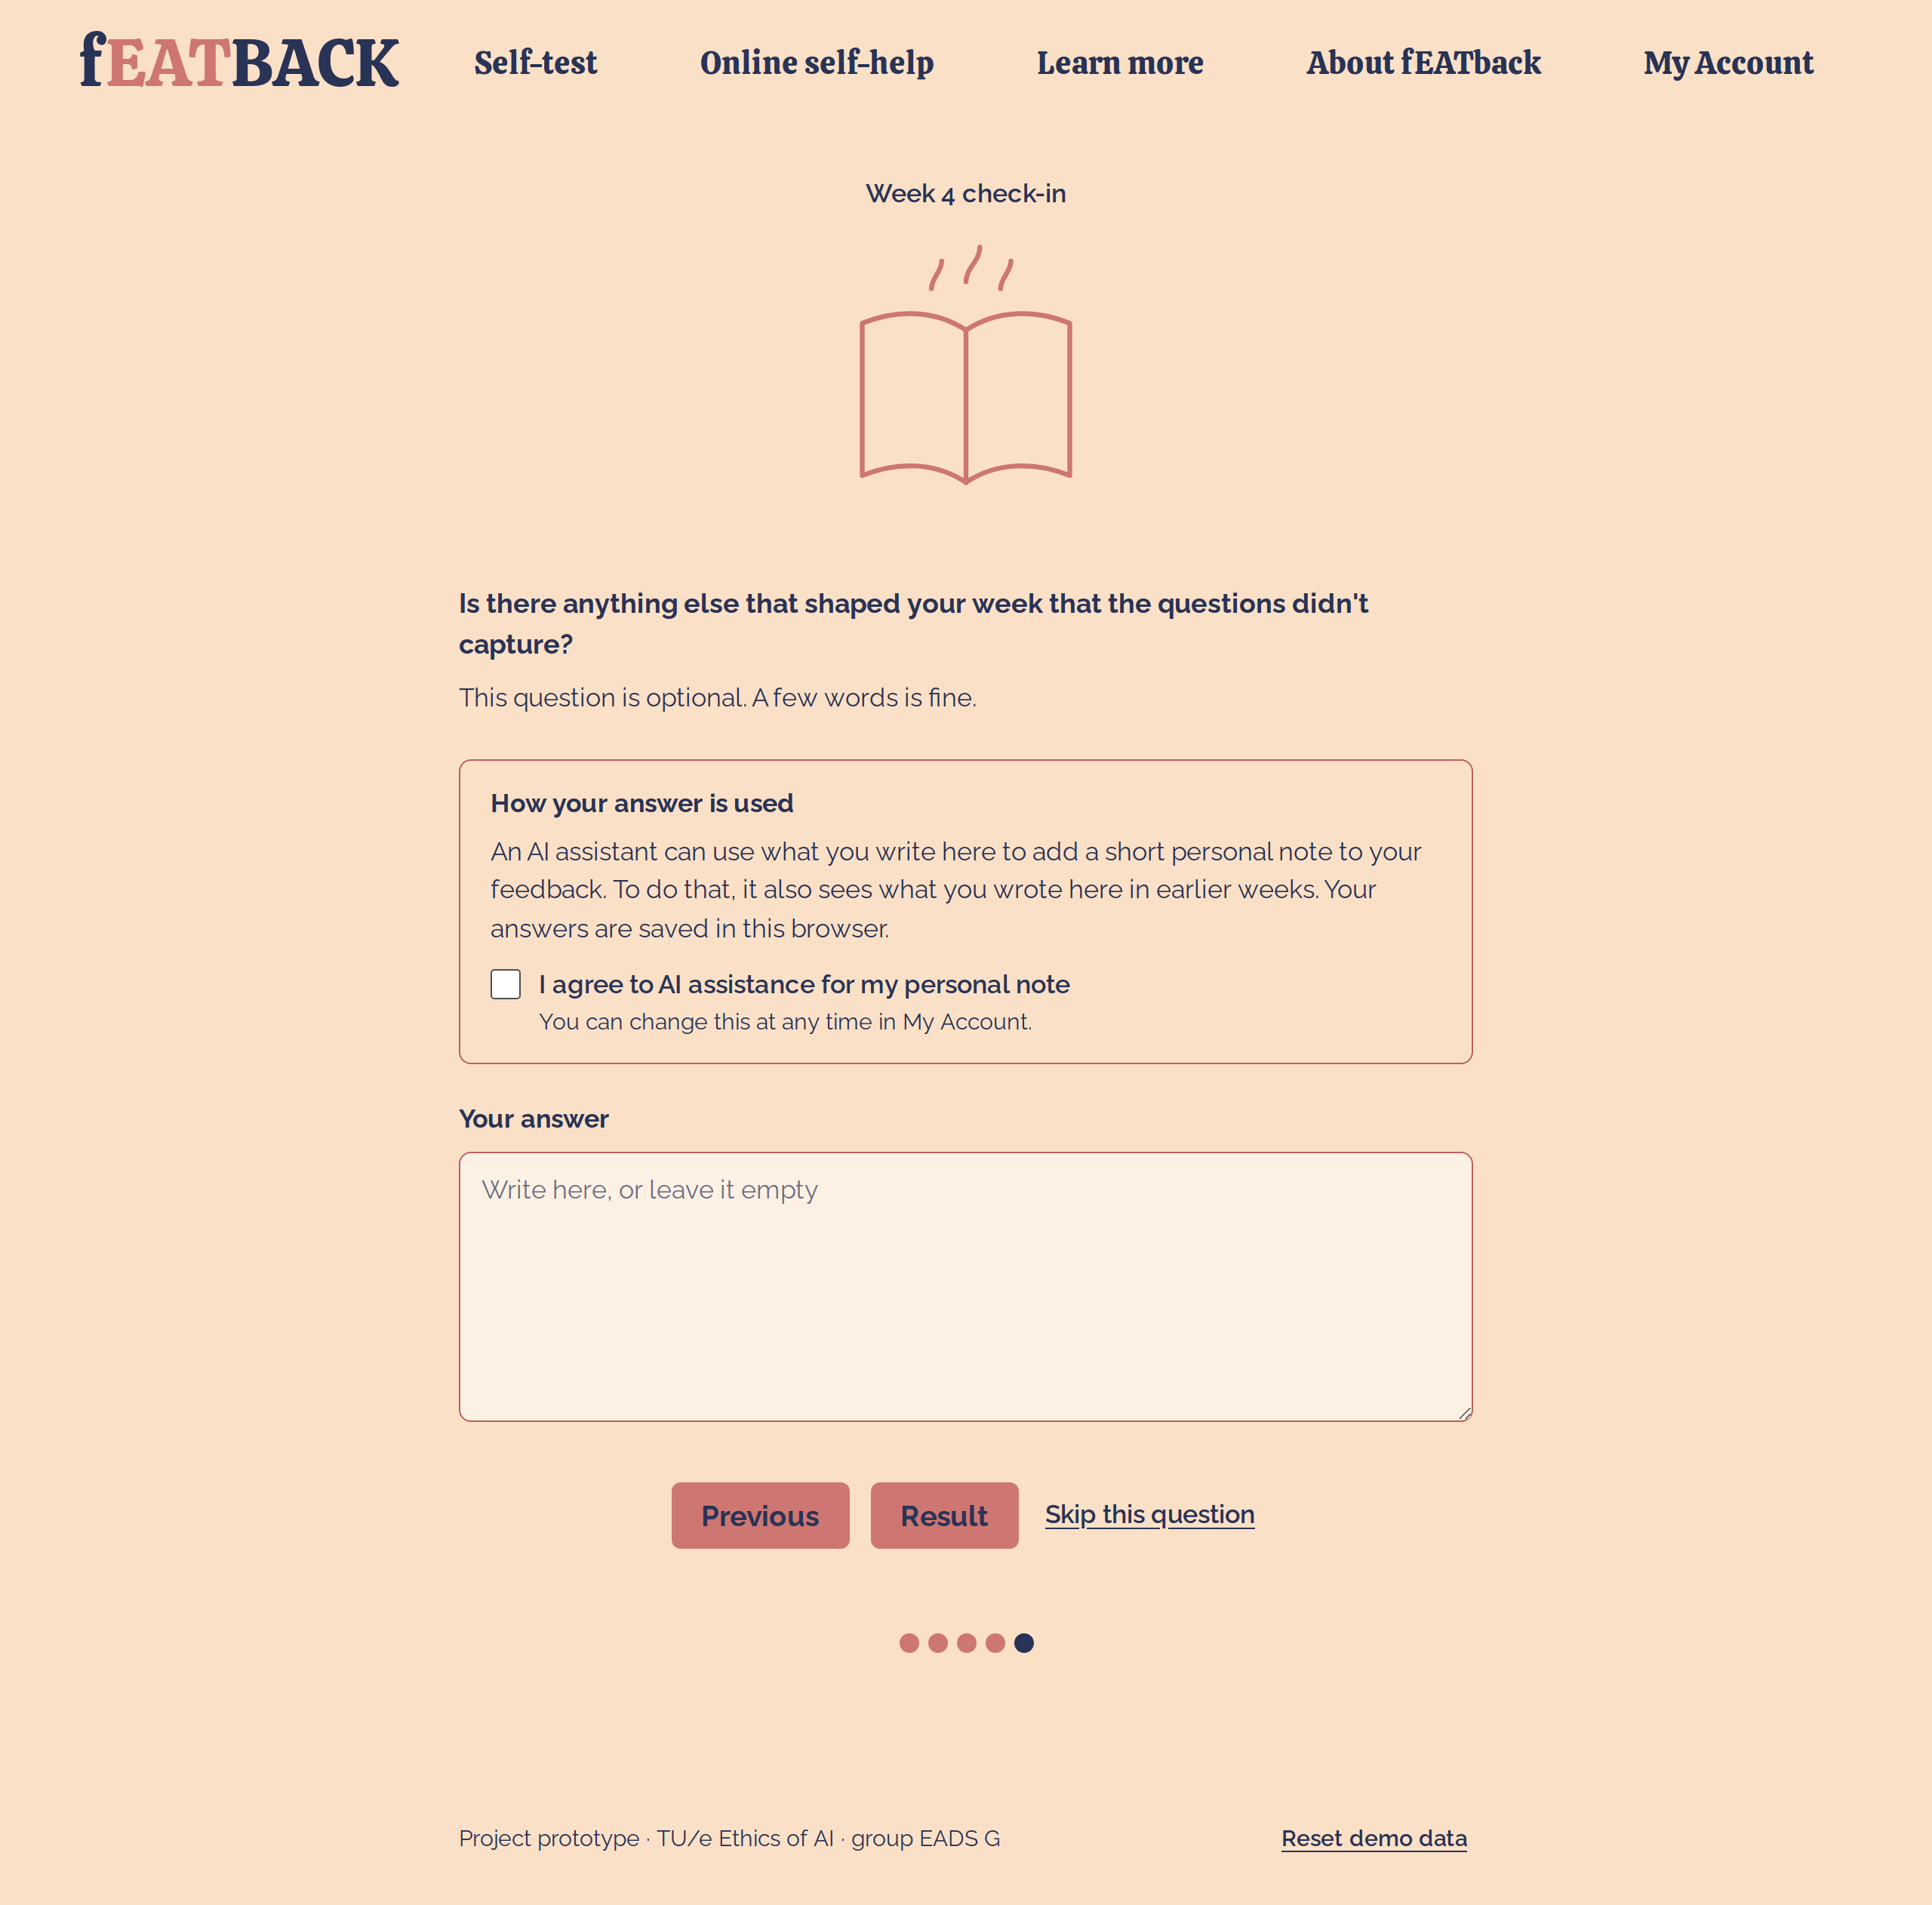
\includegraphics[width=\linewidth, trim=590 1087 590 760, clip]{q5_unticked.png}};
  \begin{scope}[x={(s.south east)}, y={(s.north west)}]
    \callout{0.979}{0.637}{1}
  \end{scope}
\end{tikzpicture}
\par\vspace{4mm}
\paneltitle{b}{Her answer and the result}
\begin{tikzpicture}
  \node[shot] (s) at (0,0) {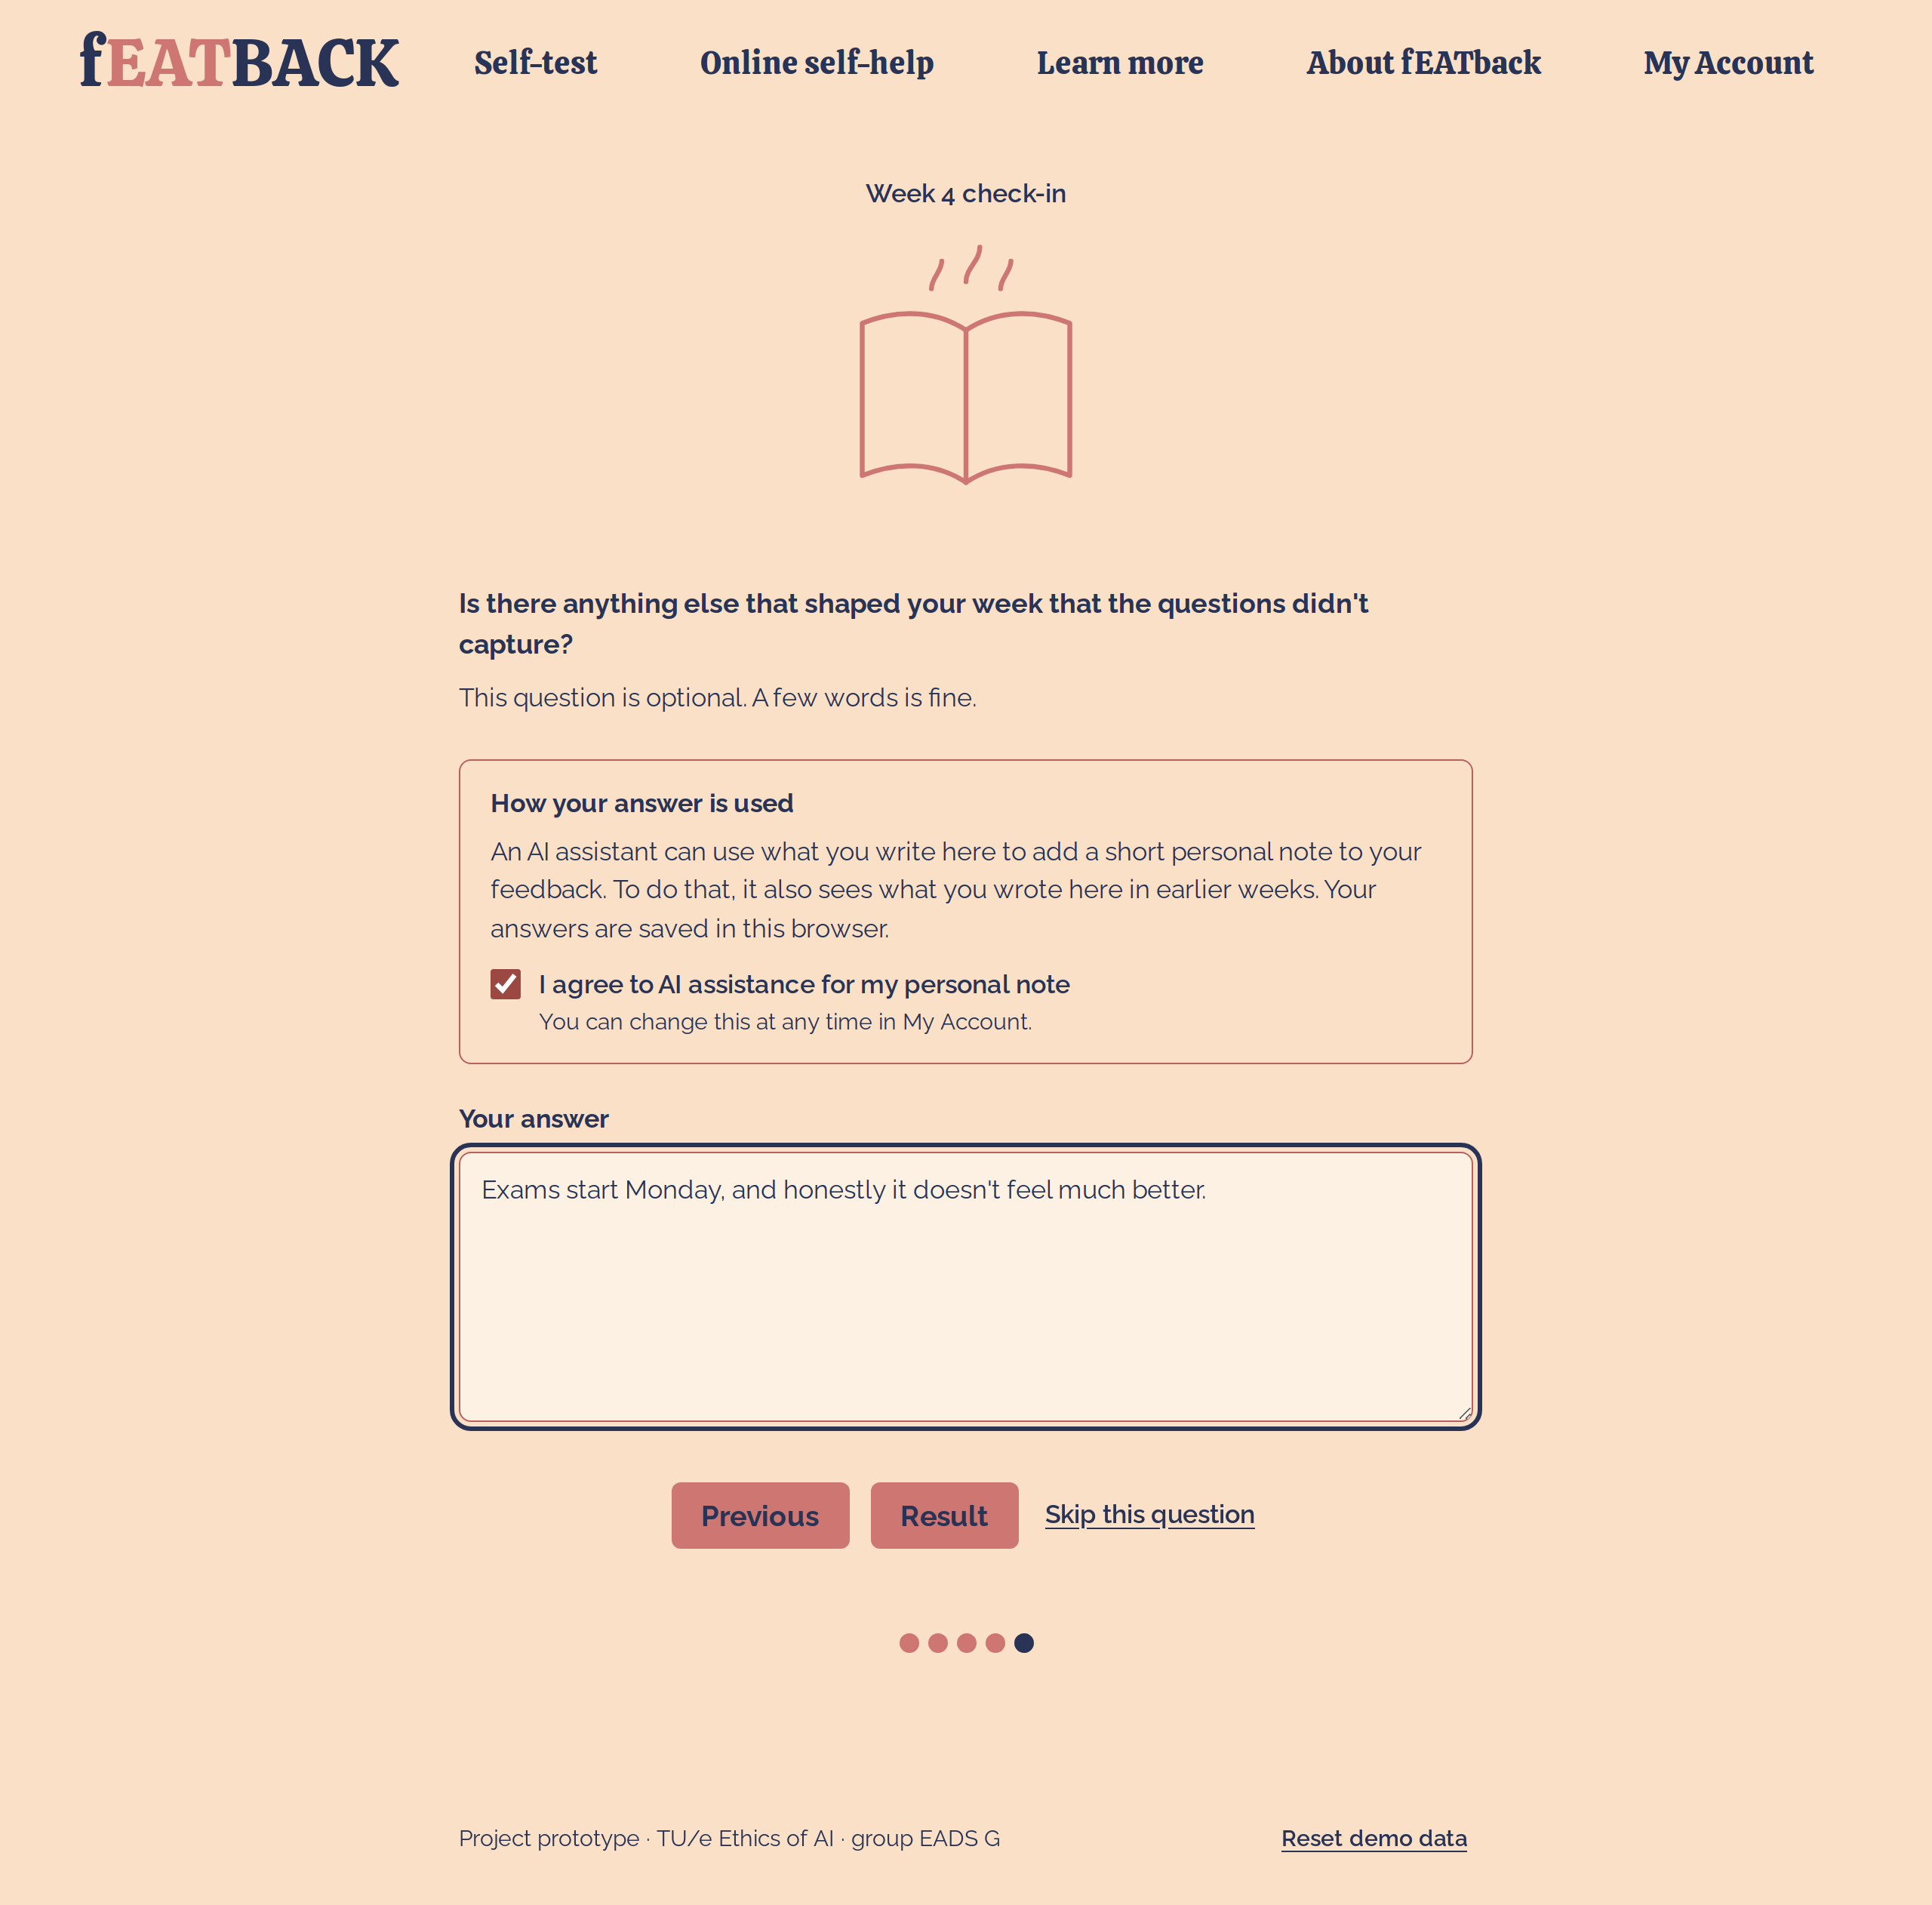
\includegraphics[width=\linewidth, trim=590 613 590 1440, clip]{q5_screen.png}};
  \begin{scope}[x={(s.south east)}, y={(s.north west)}]
    \callout{0.979}{0.817}{2}
  \end{scope}
\end{tikzpicture}
\par\vspace{1.5mm}
\begin{tikzpicture}
  \node[shot] (s) at (0,0) {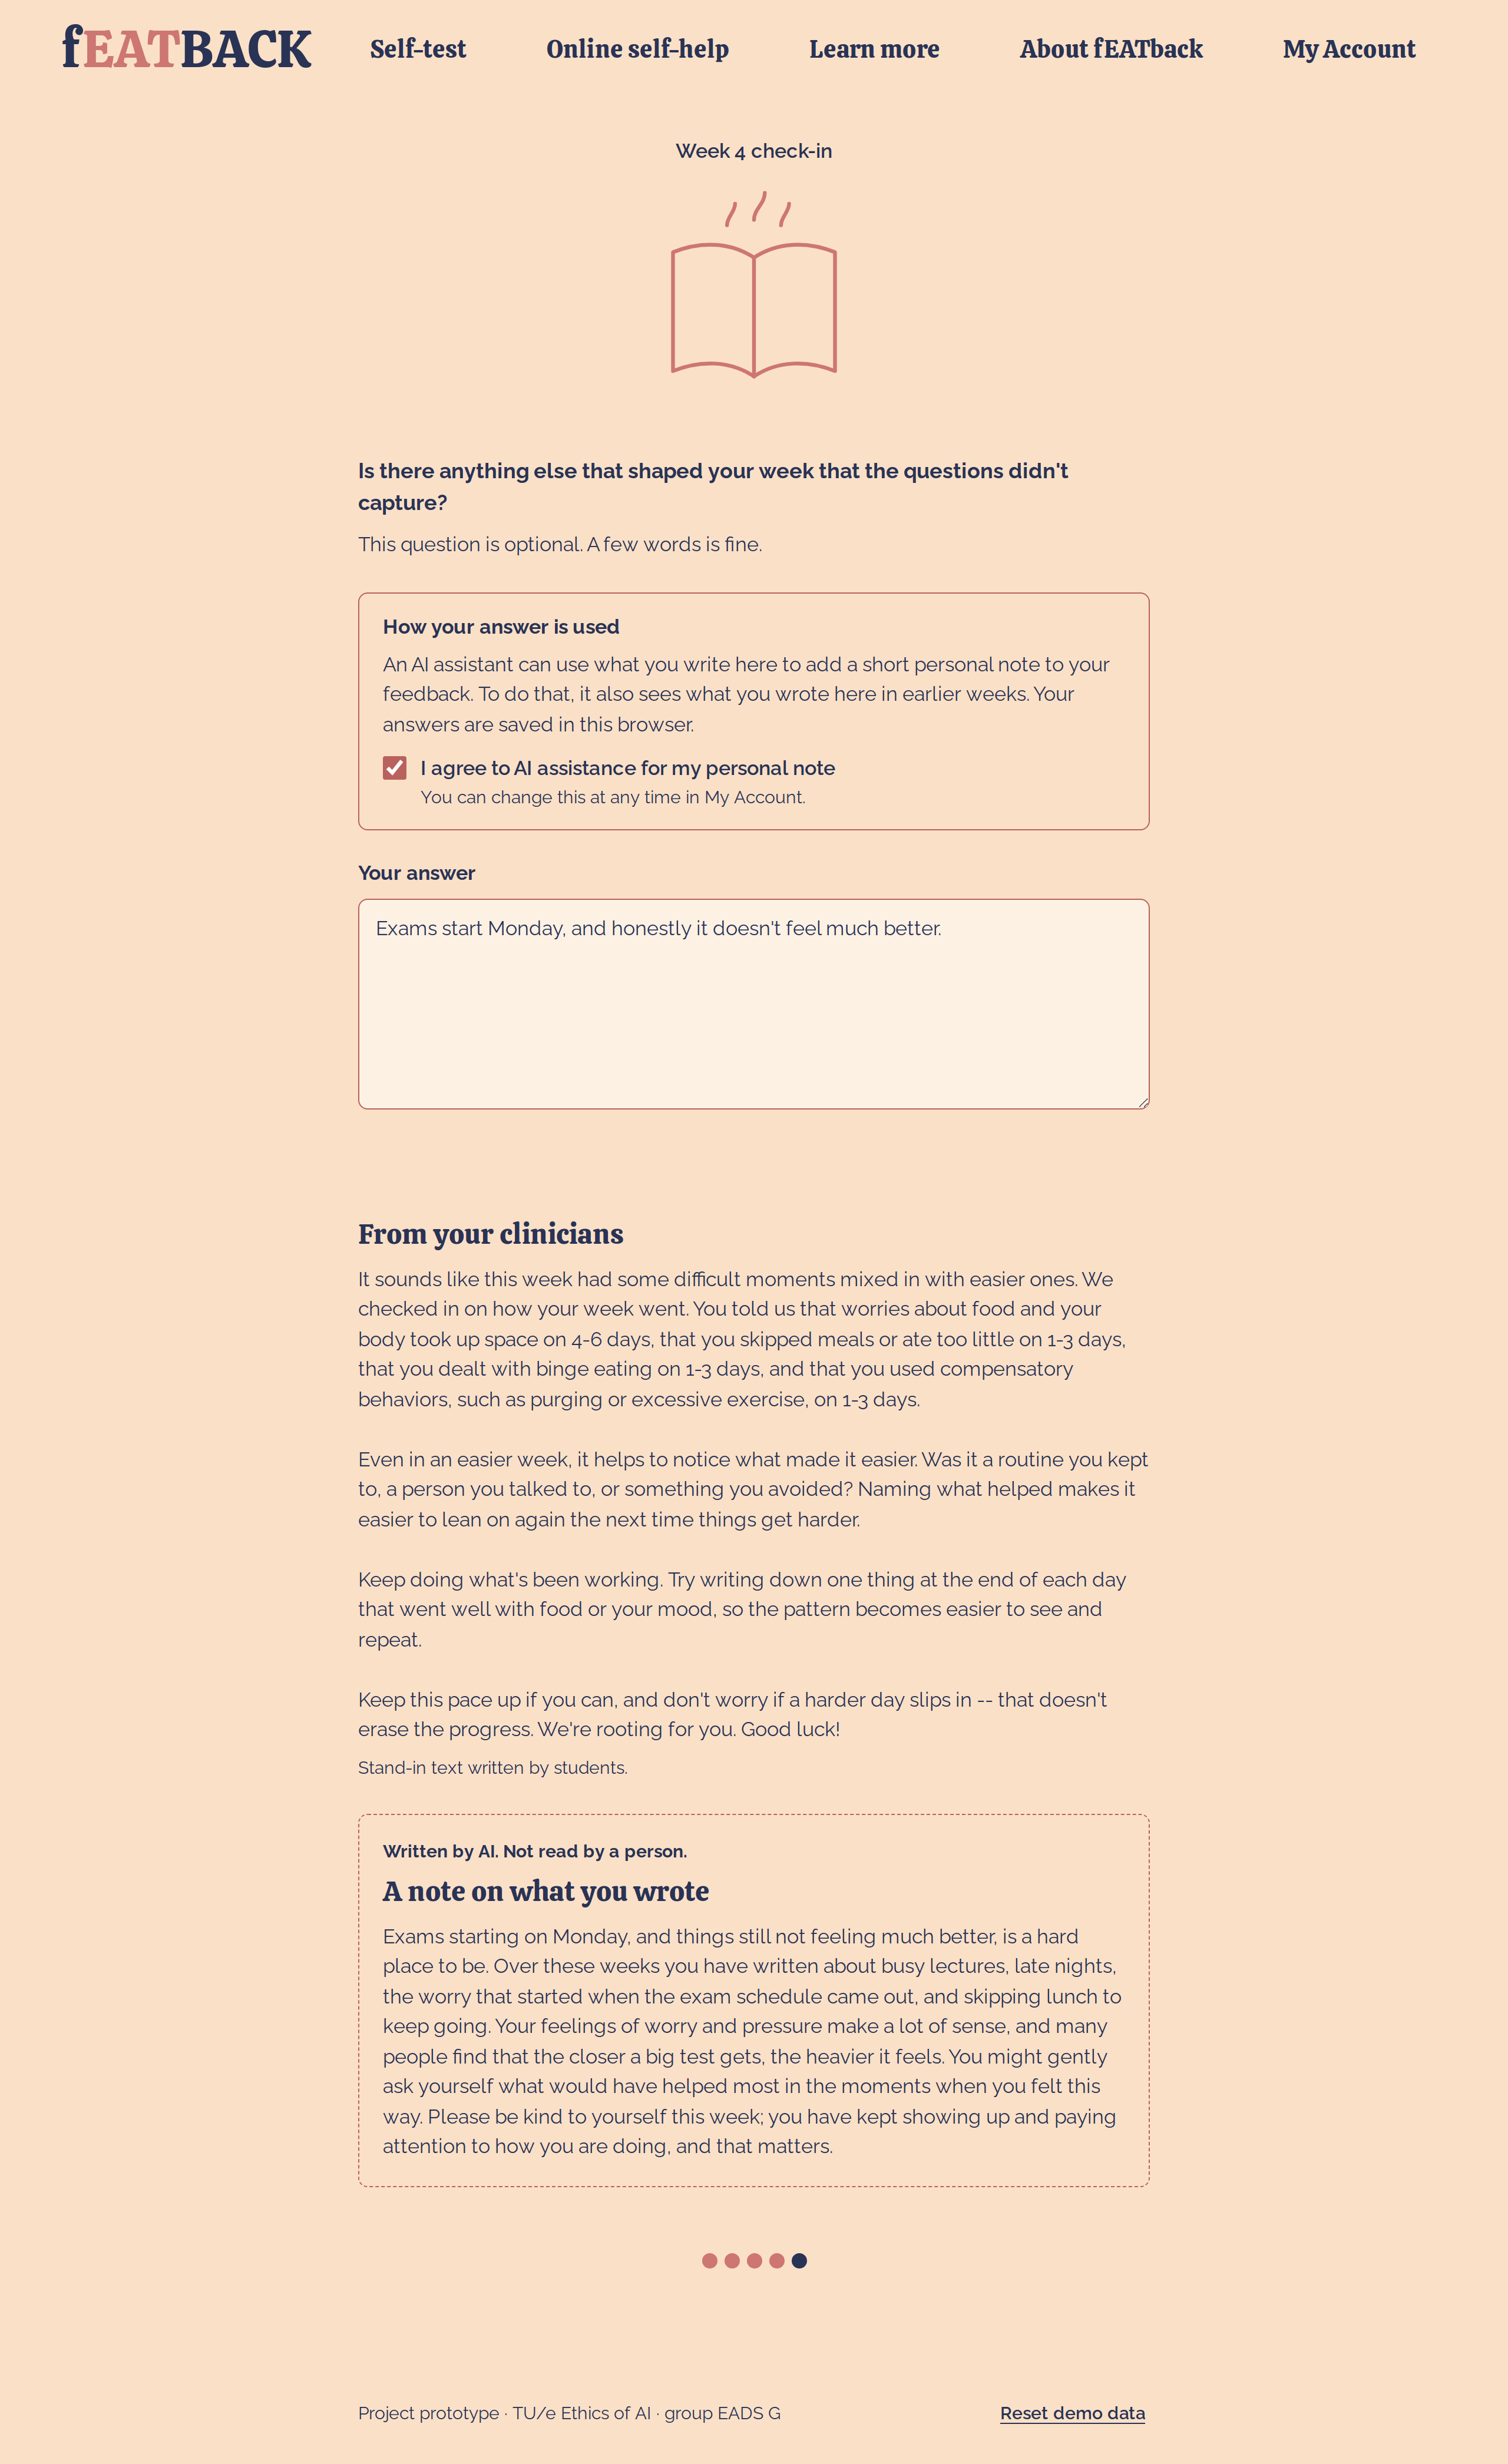
\includegraphics[width=\linewidth, trim=590 443 590 2046, clip]{result_screen.png}};
  \begin{scope}[x={(s.south east)}, y={(s.north west)}]
    \callout{0.979}{0.983}{3}
    \callout{0.979}{0.390}{4}
  \end{scope}
\end{tikzpicture}
\end{minipage}%
\hfill
% ============ Right column: other weeks and edge cases ============
\begin{minipage}[t]{0.47\textwidth}
\colhead{Week 5 and when something goes wrong}
\paneltitle{c}{Week 5, where the note looks back}
\begin{tikzpicture}
  \node[shot] (s) at (0,0) {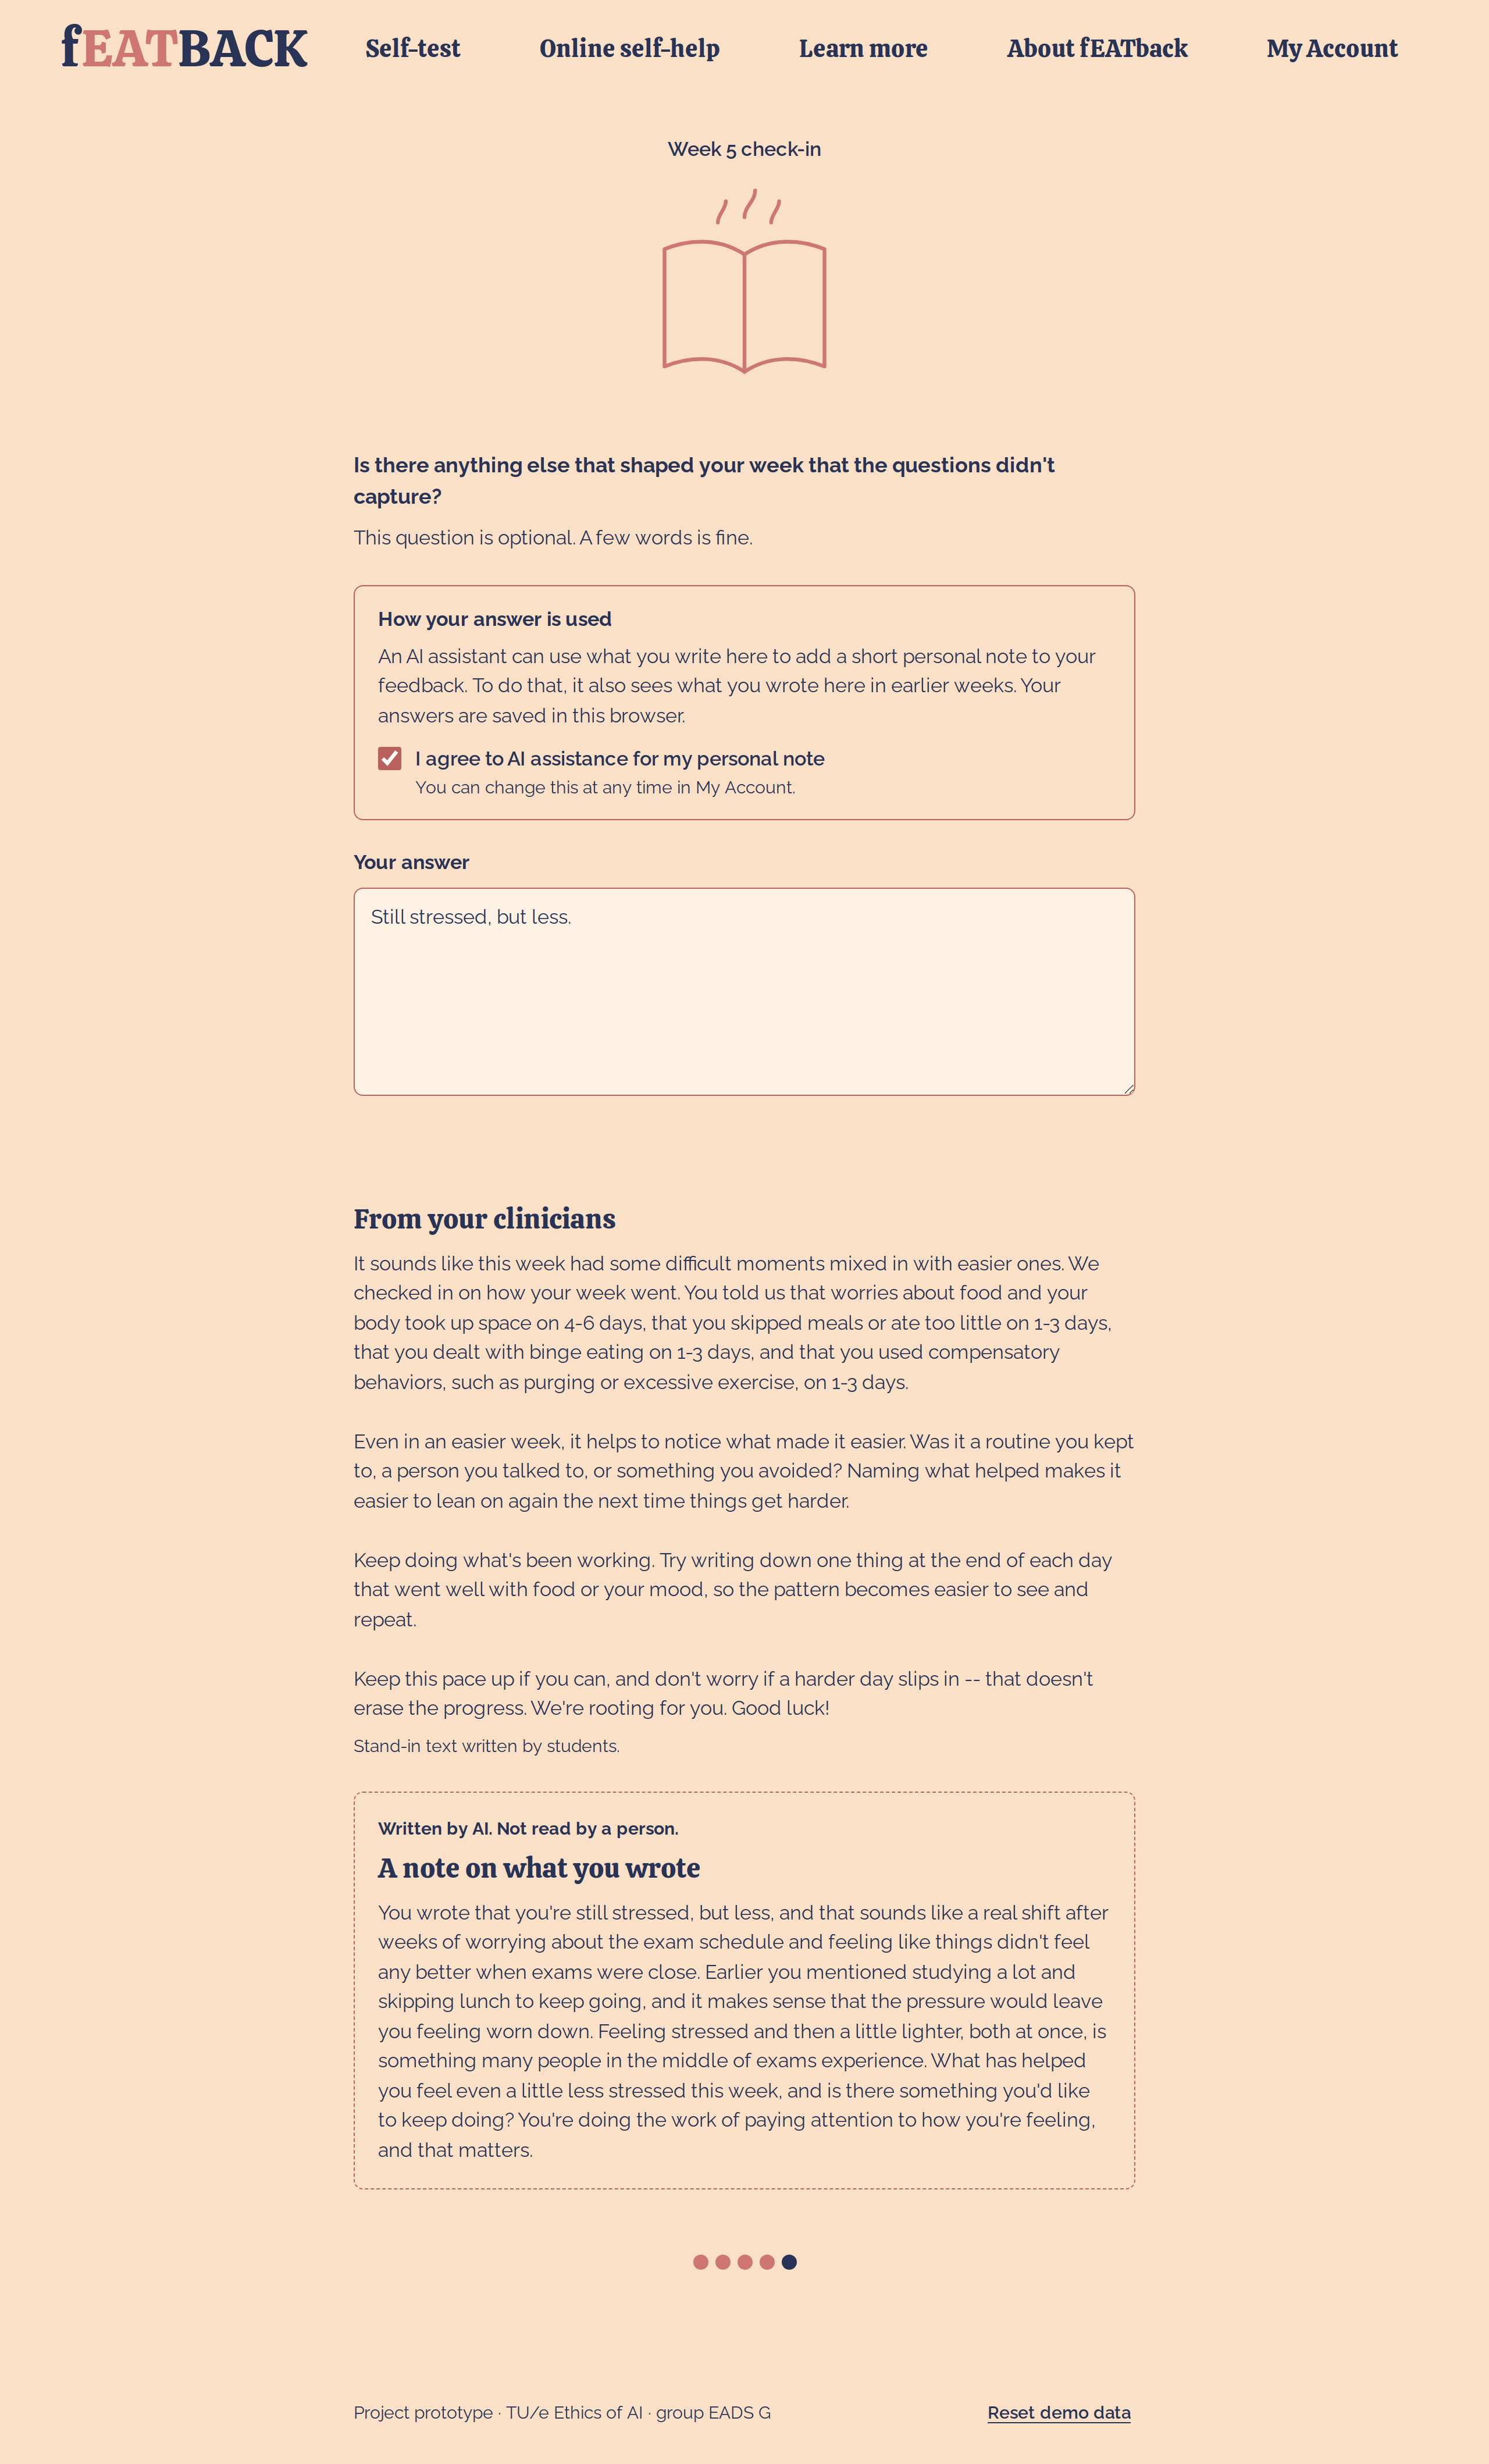
\includegraphics[width=\linewidth, trim=590 2325 590 1440, clip]{result_week5.png}};
\end{tikzpicture}
\par\vspace{1.5mm}
\begin{tikzpicture}
  \node[shot] (s) at (0,0) {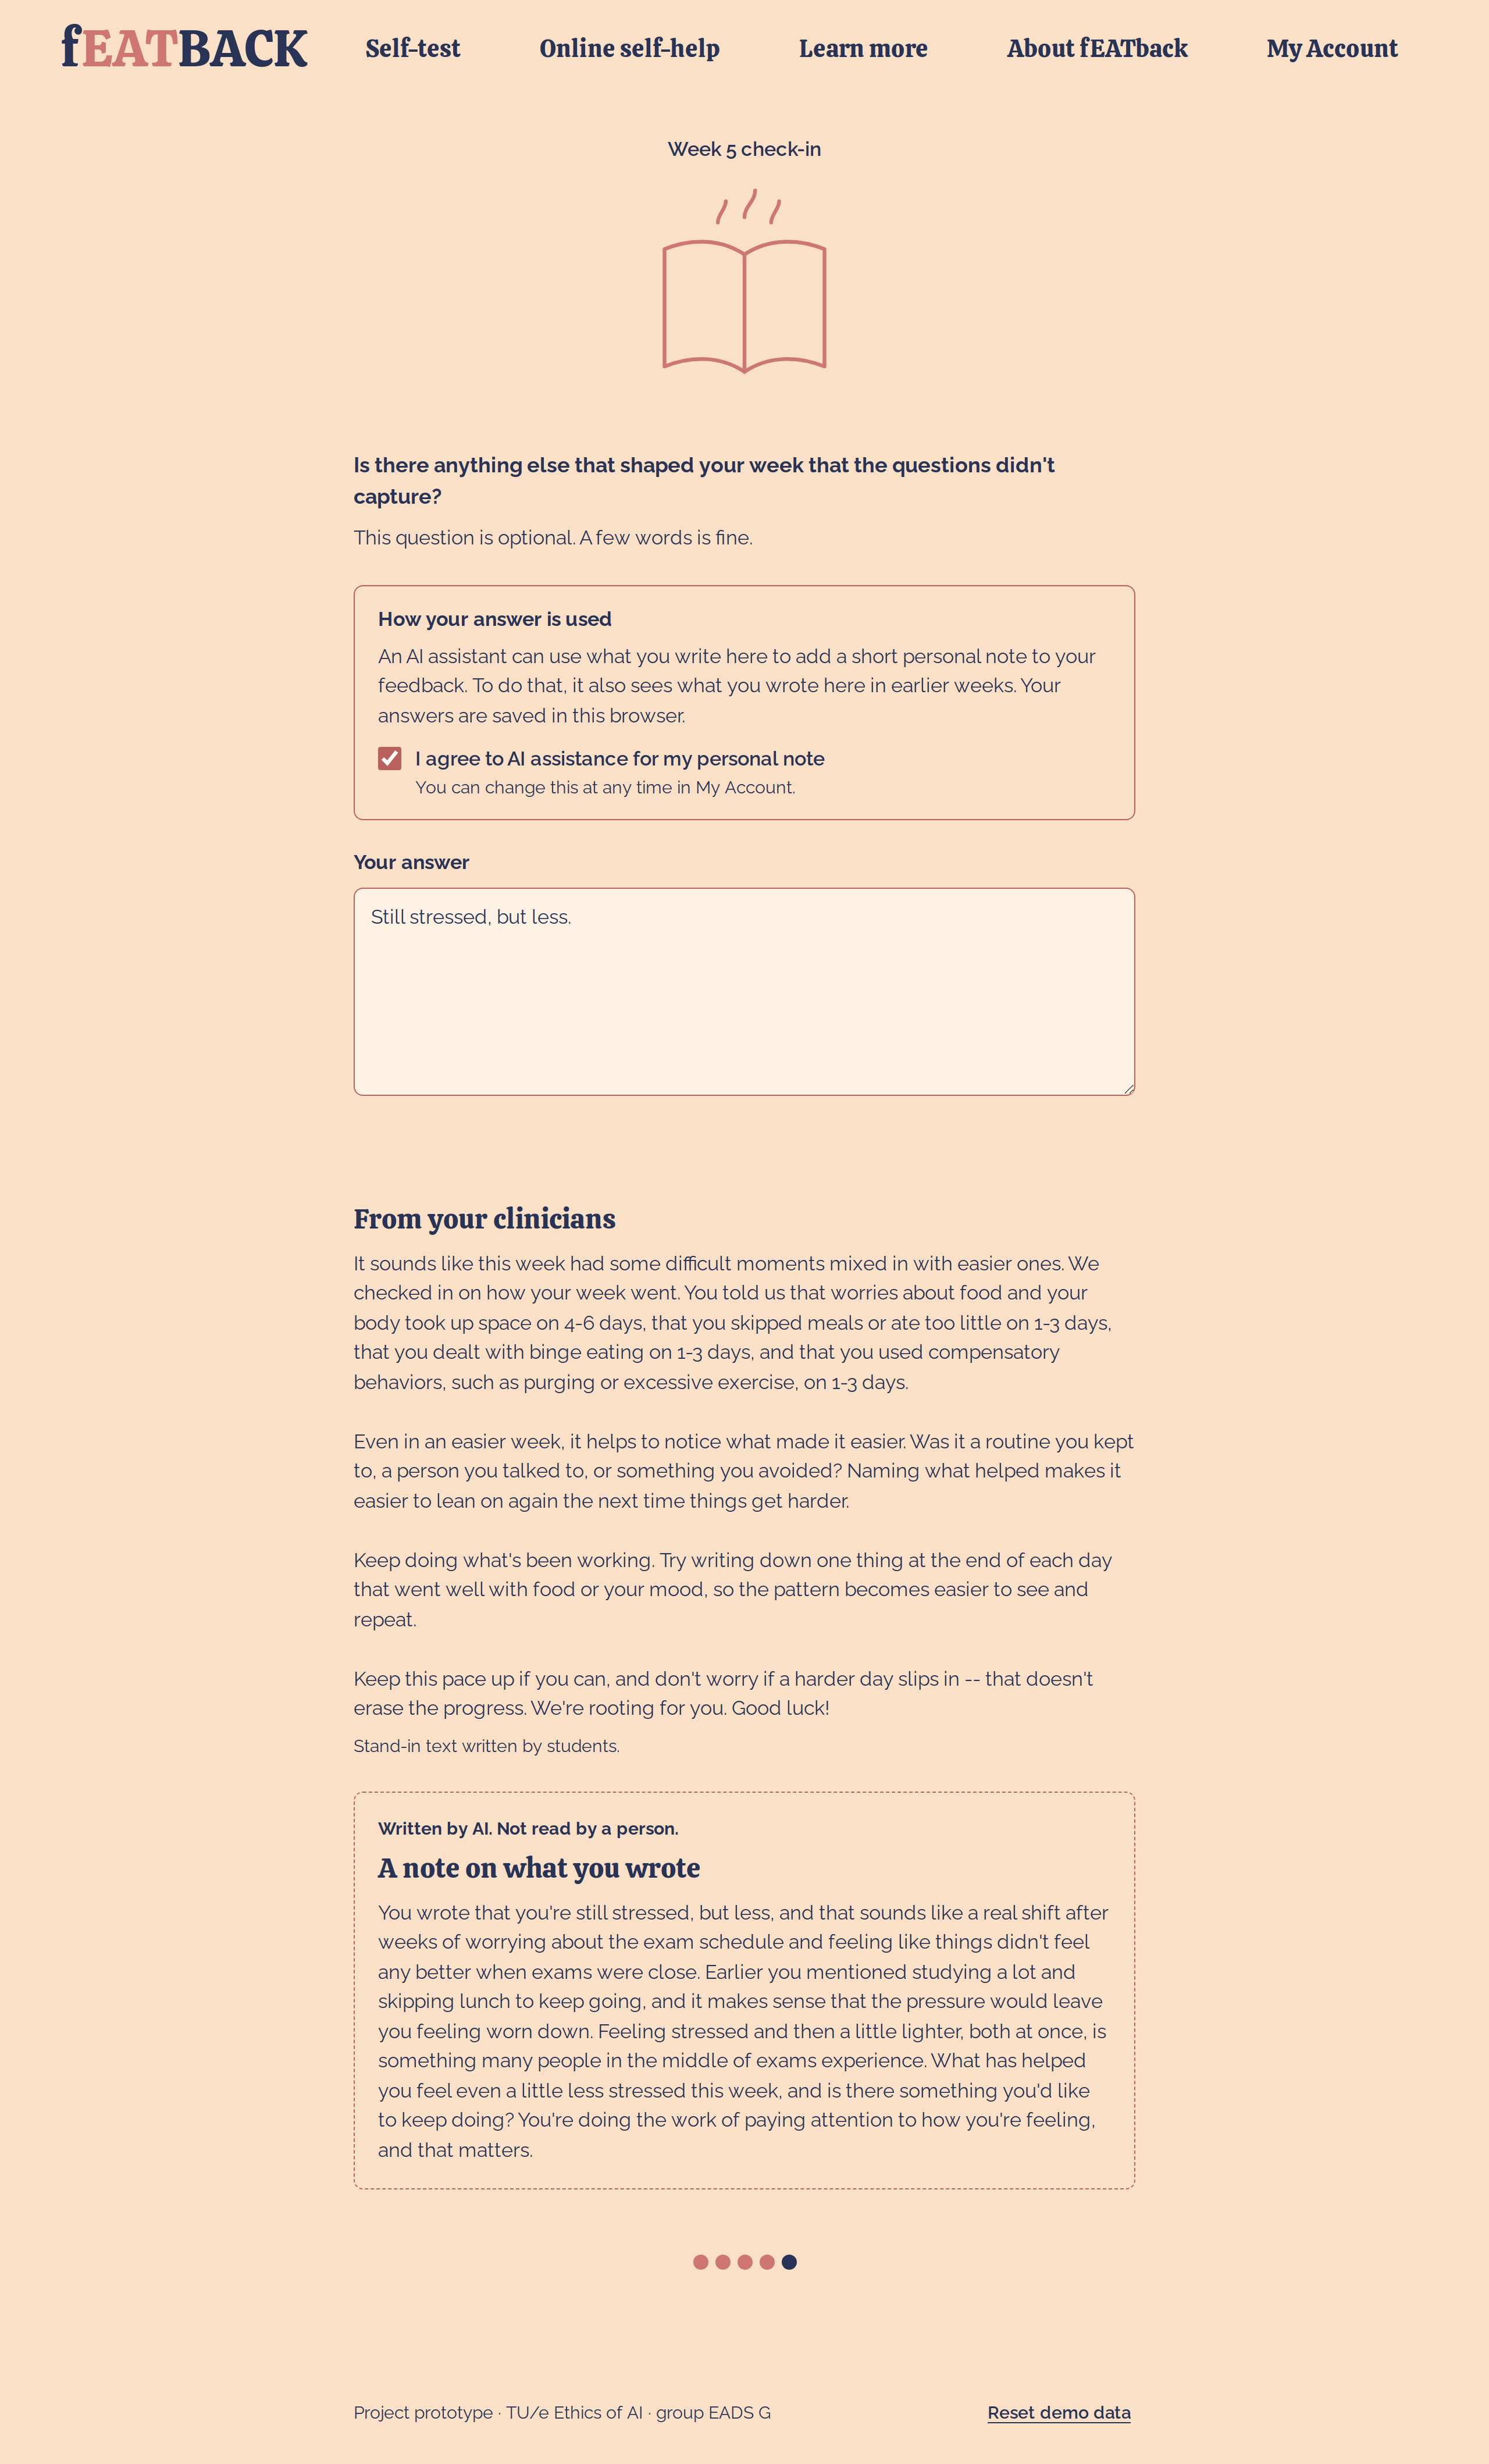
\includegraphics[width=\linewidth, trim=590 445 590 3052, clip]{result_week5.png}};
\end{tikzpicture}
\par\vspace{4mm}
\paneltitle{d}{Model off or note rejected}
\begin{tikzpicture}
  \node[shot] (s) at (0,0) {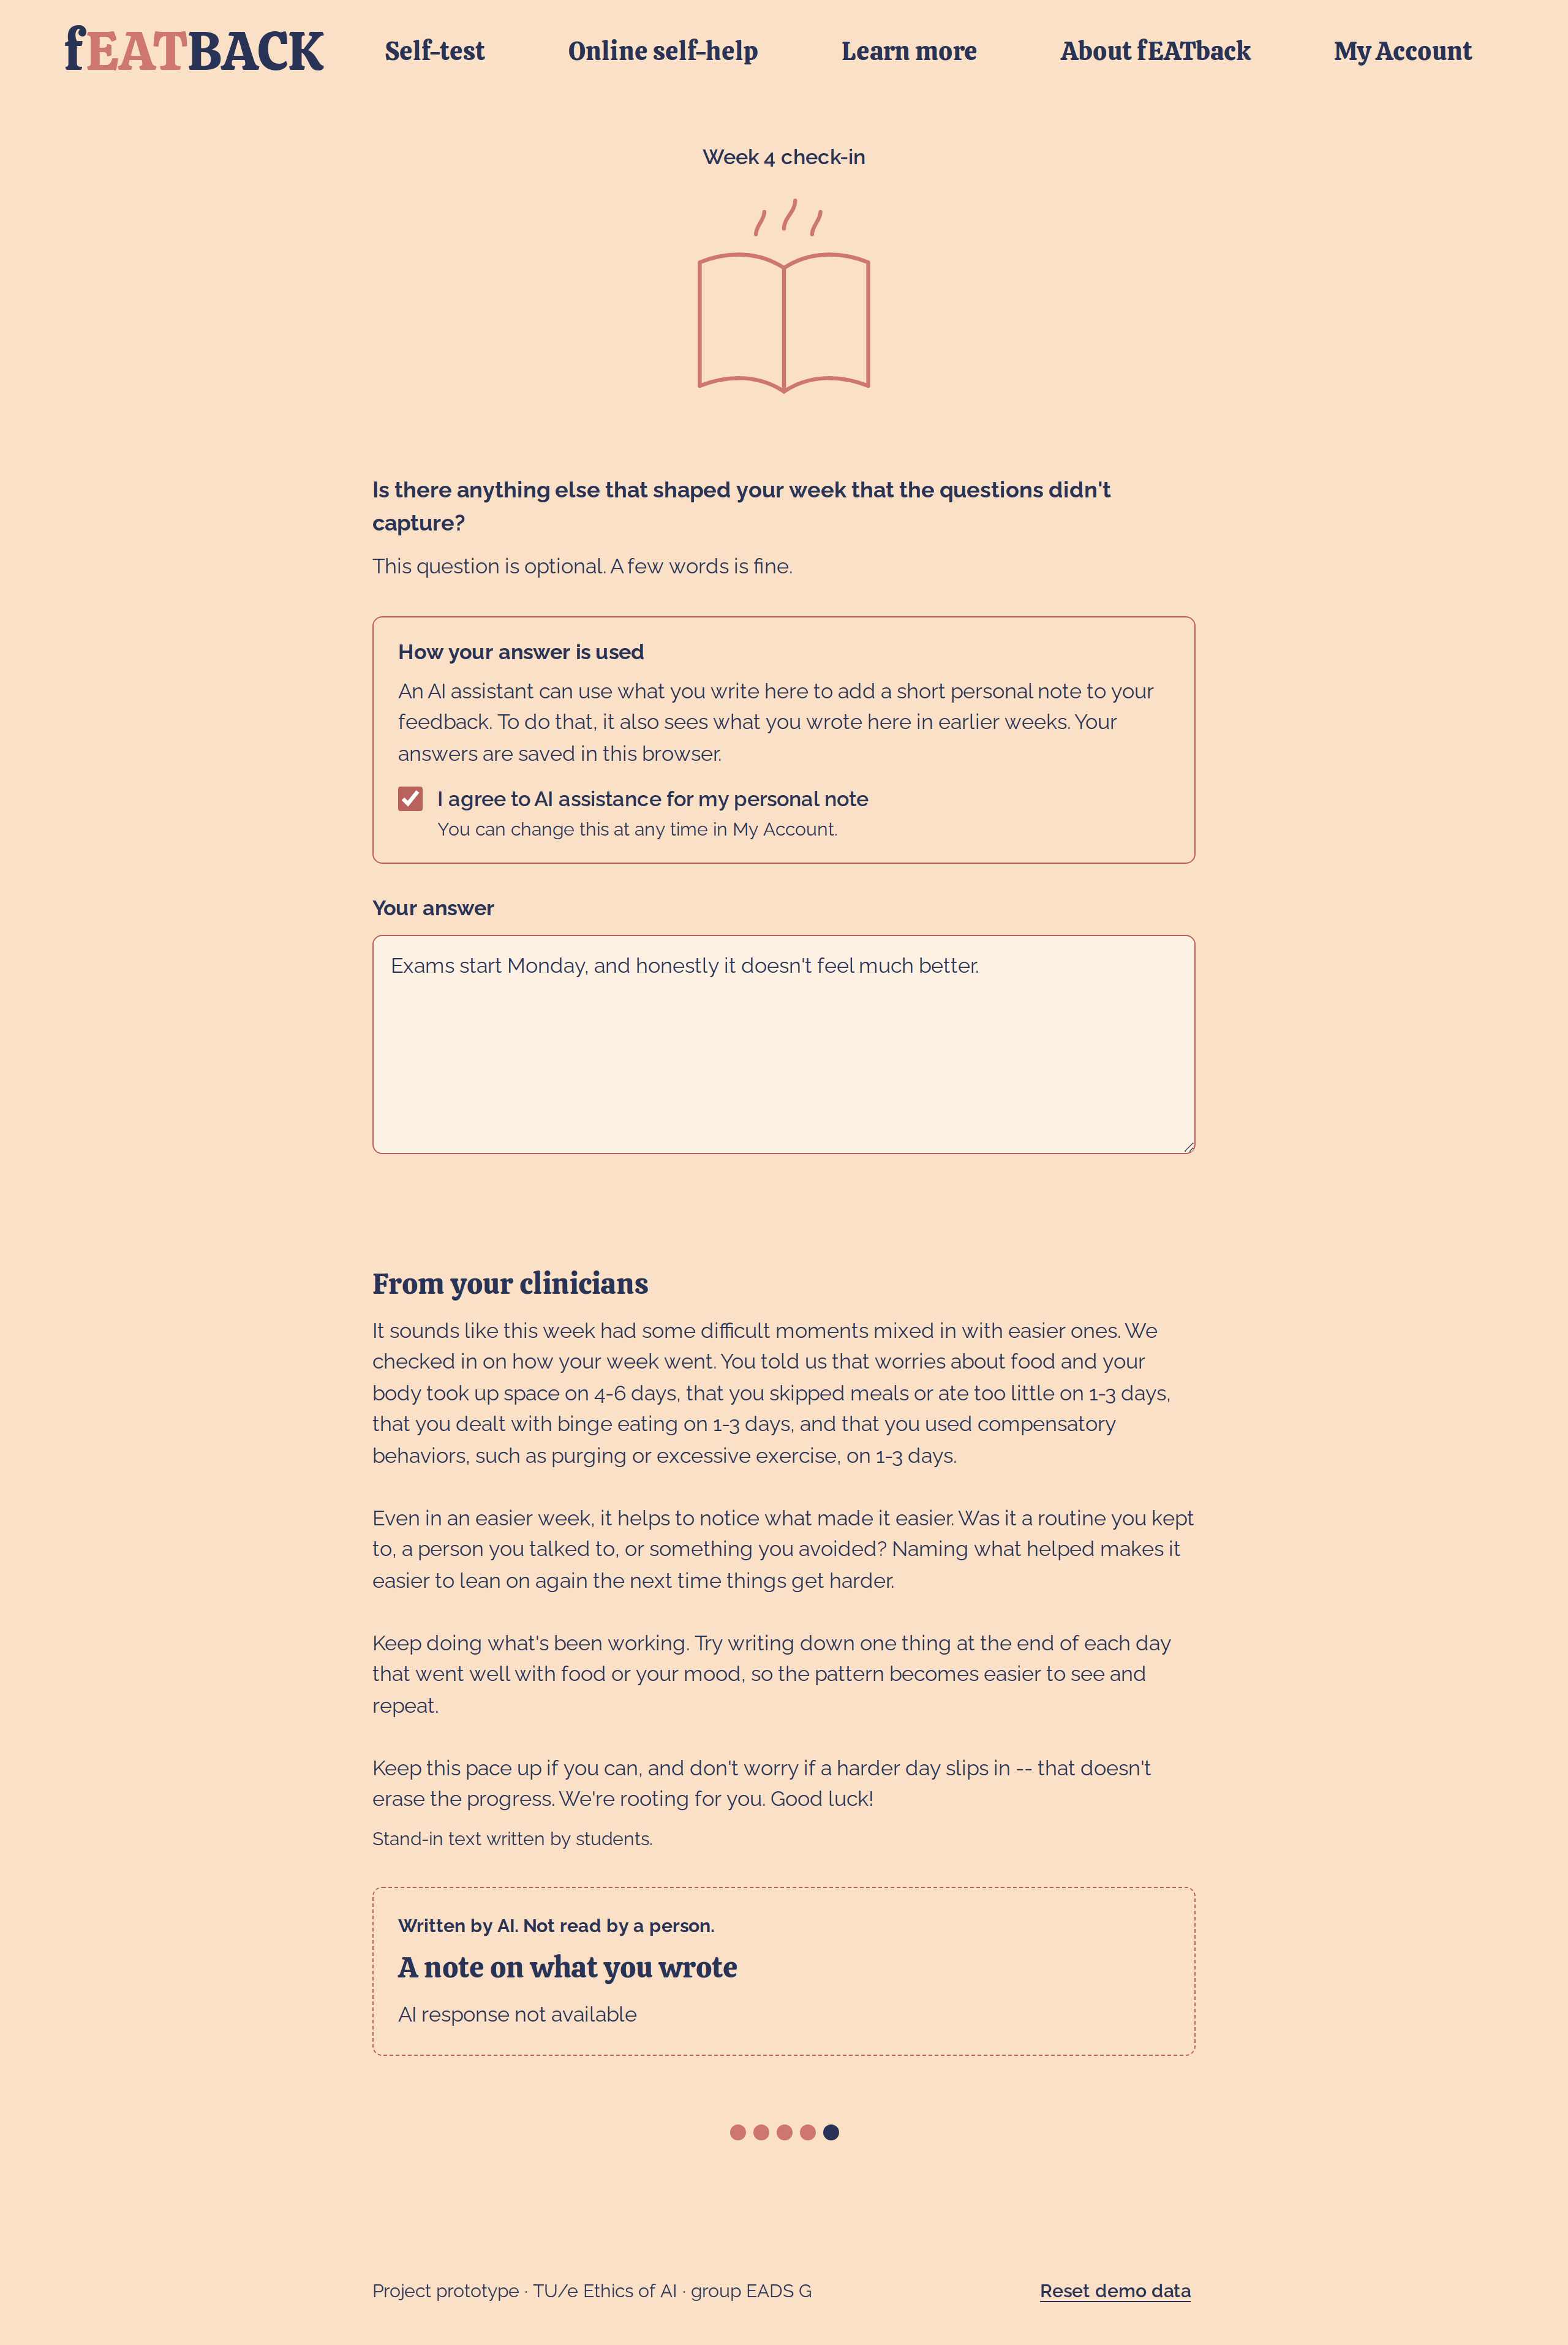
\includegraphics[width=\linewidth, trim=590 445 590 3052, clip]{fallback.png}};
  \begin{scope}[x={(s.south east)}, y={(s.north west)}]
    \callout{0.979}{0.915}{5}
  \end{scope}
\end{tikzpicture}
\par\vspace{4mm}
\paneltitle{e}{An answer with signs of acute risk}
\begin{tikzpicture}
  \node[shot] (s) at (0,0) {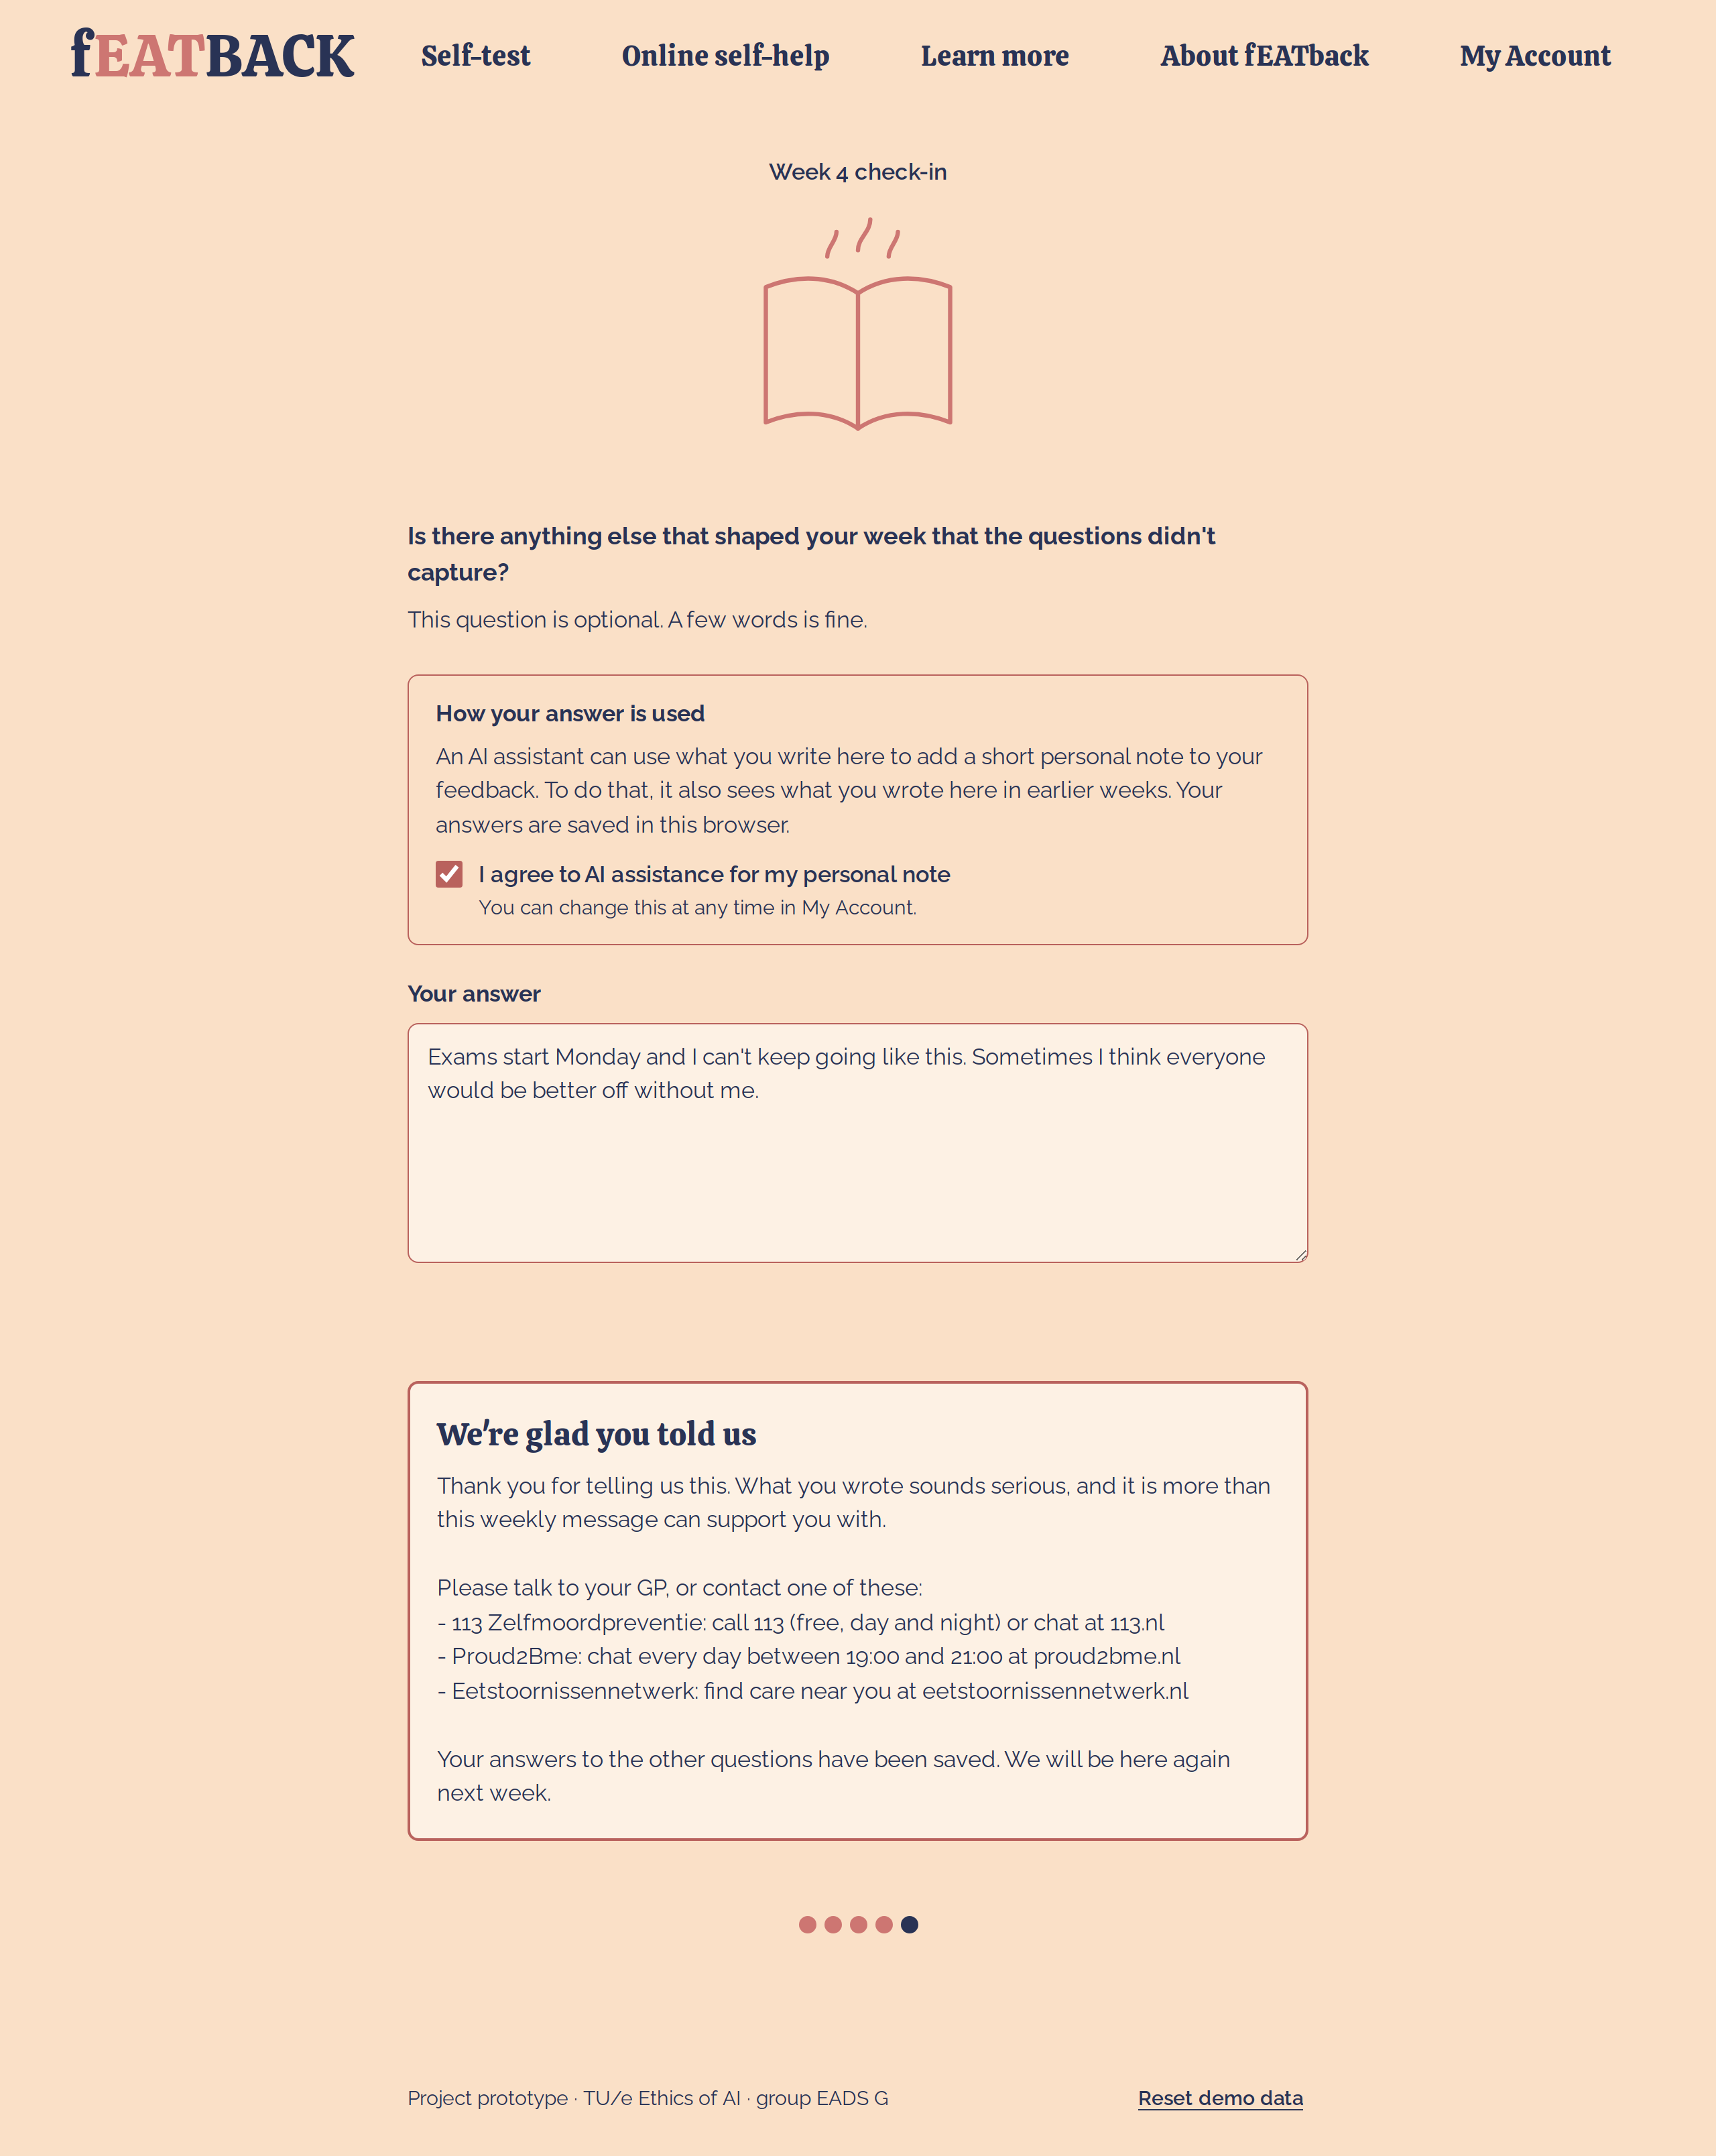
\includegraphics[width=\linewidth, trim=590 1305 590 1440, clip]{acute.png}};
\end{tikzpicture}
\par\vspace{1.5mm}
\begin{tikzpicture}
  \node[shot] (s) at (0,0) {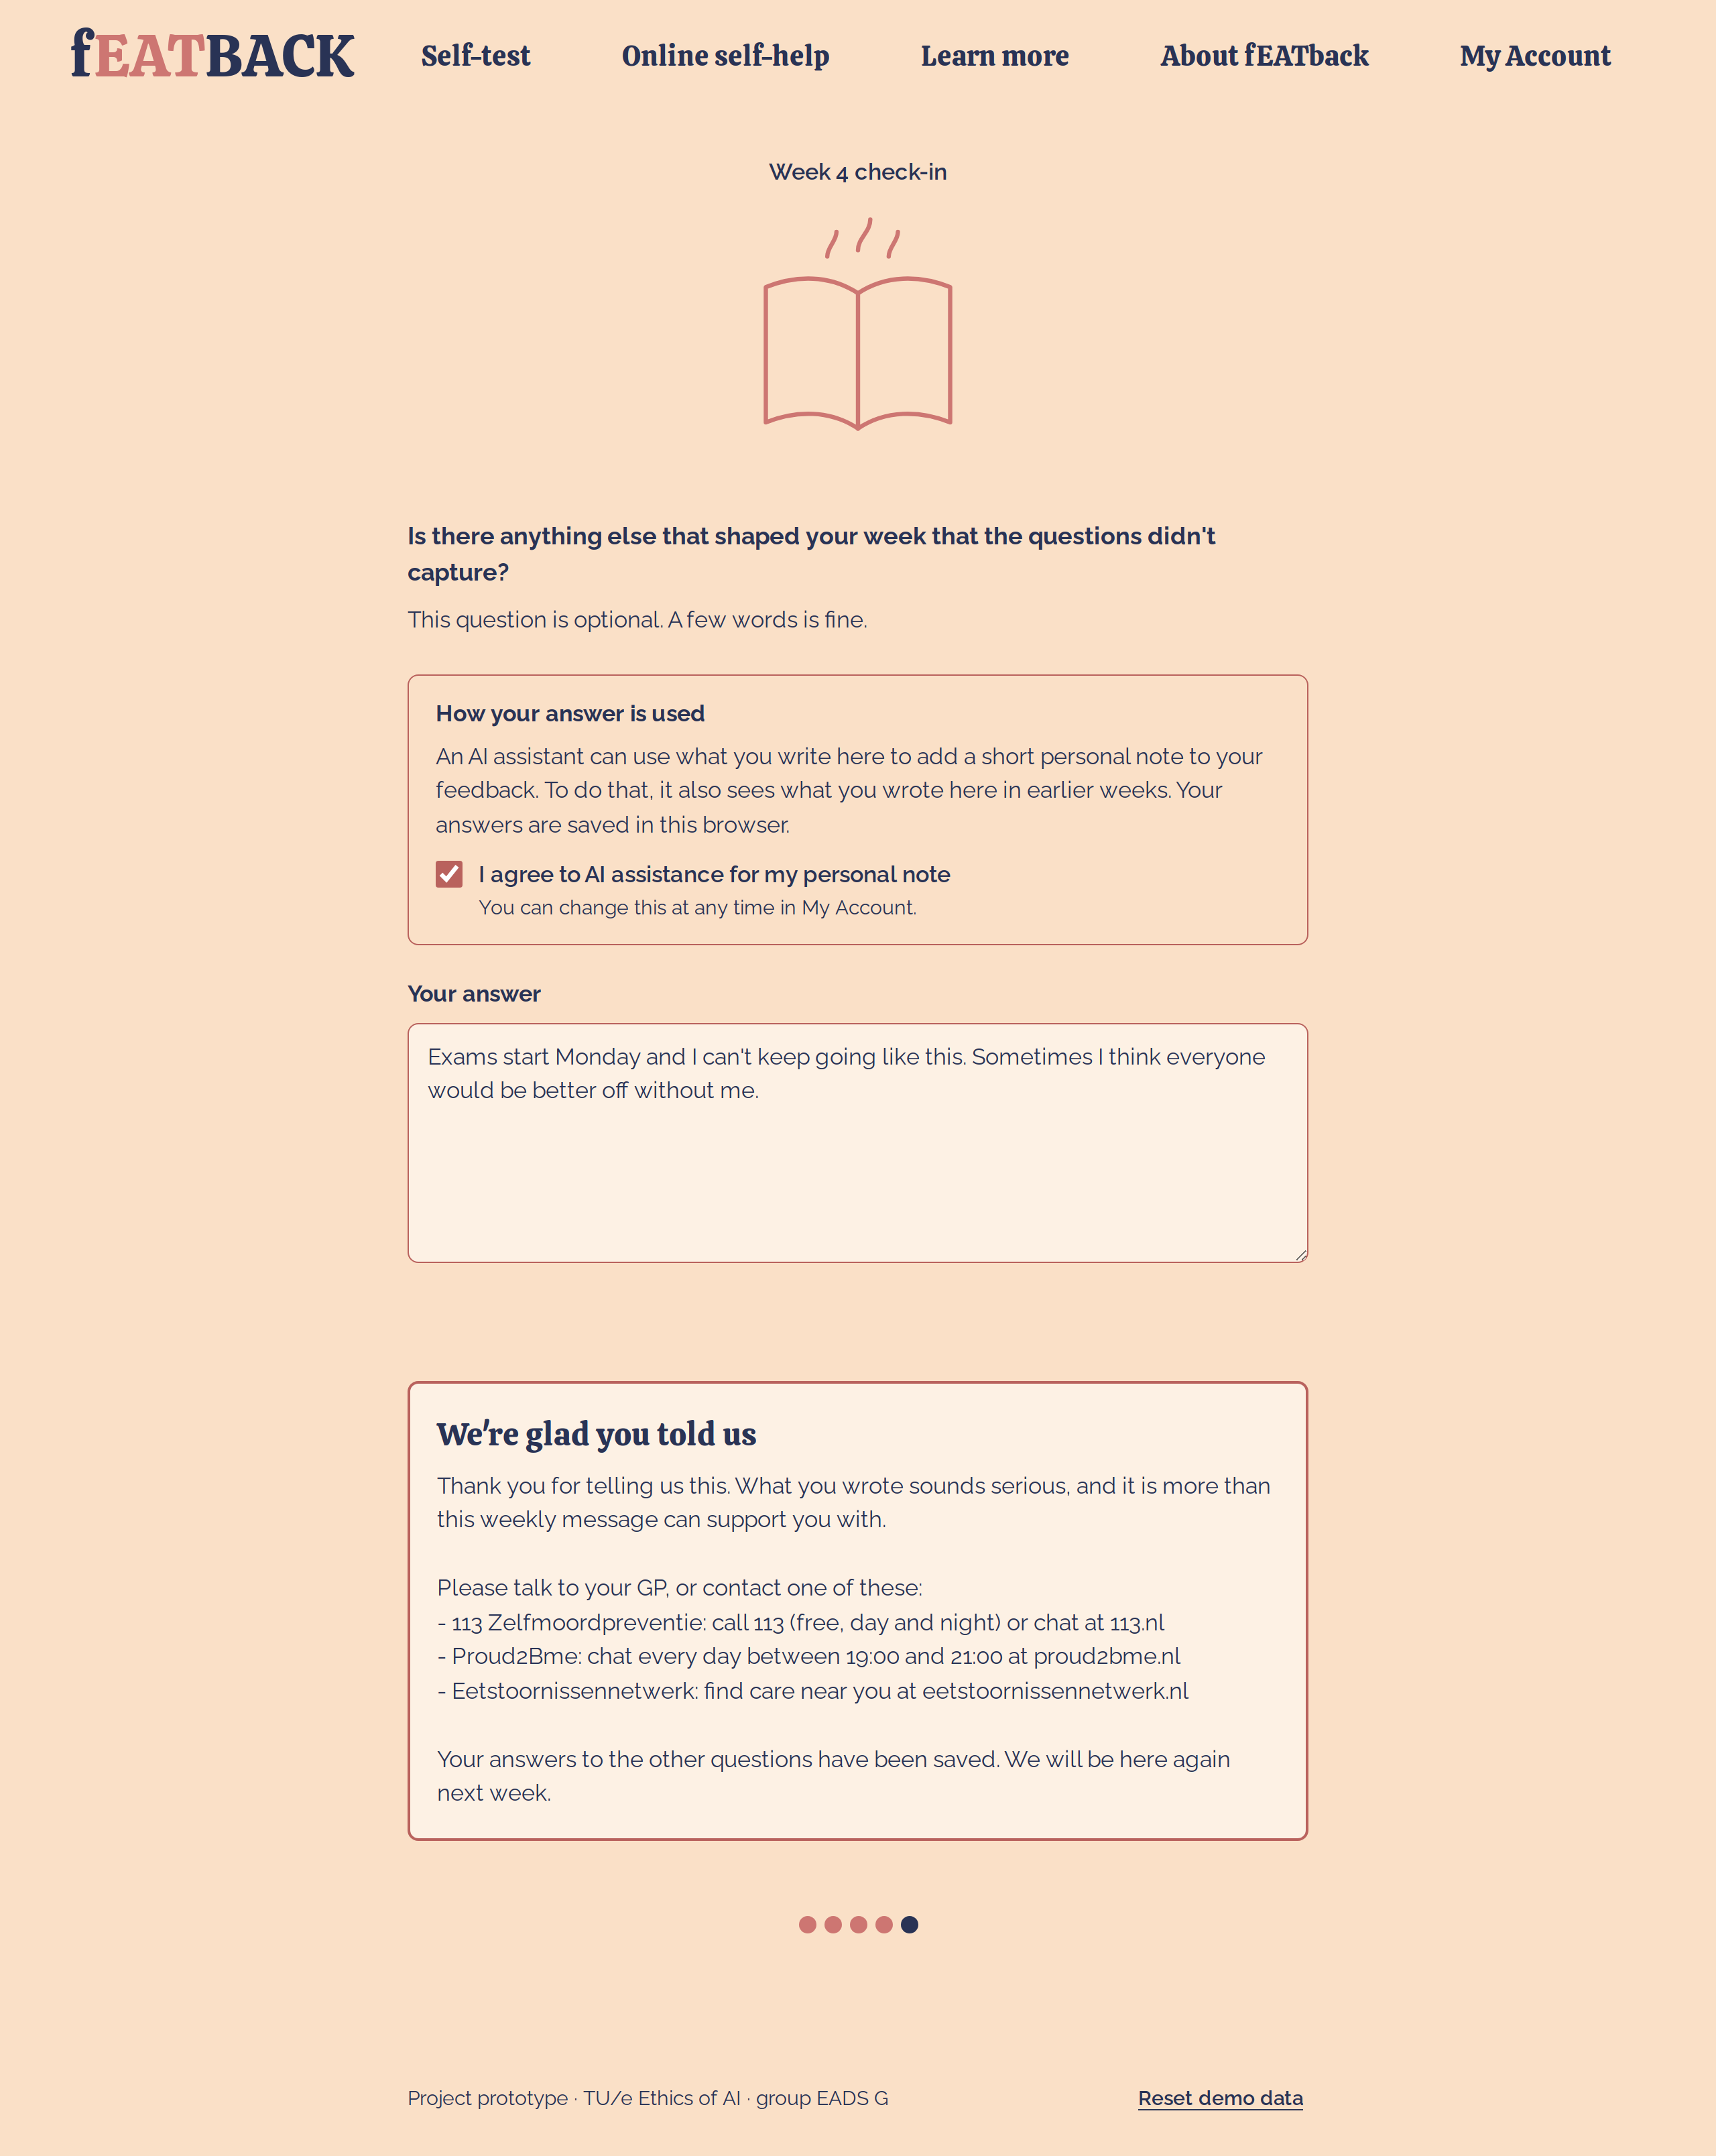
\includegraphics[width=\linewidth, trim=590 443 590 2032, clip]{acute.png}};
  \begin{scope}[x={(s.south east)}, y={(s.north west)}]
    \callout{0.979}{0.962}{6}
  \end{scope}
\end{tikzpicture}
\end{minipage}

\vspace{5mm}
% ---- Key: one entry per callout, aligned with the two columns ----
\newcommand{\keyline}[2]{\key{#1}\hspace{2mm}#2\par\vspace{1.2mm}}
{\footnotesize\sffamily
\begin{minipage}[t]{0.47\textwidth}
\keyline{1}{Consent box starts unticked (part 3)}
\keyline{2}{Answer stored for the trend (part 3)}
\keyline{3}{Stand-in bank message (part 1)}
\end{minipage}\hfill
\begin{minipage}[t]{0.47\textwidth}
\keyline{4}{Label on every AI note (part 2)}
\keyline{5}{Fixed fallback text we wrote (part 1)}
\keyline{6}{Gate takes the more severe label (part 1)}
\end{minipage}}

\vspace{2mm}
\caption{Maren's check-ins from Section~\ref{sec:narrative} as they appear on screen. Part numbers in the key
point to the Responsible Innovation statement. The AI notes in (b) and (c) are real
output from our fine-tuned writer model, run on 12 October 2026. The bank message, Maren
and her earlier answers are made up for the demo.}
\label{fig:mockup}
\end{figure}
.
% Needs tikz (loaded by todonotes in main.tex), graphicx and float.

% ---- Figure style ----------------------------------------------------------
\definecolor{fbnavy}{HTML}{283357}
\tikzset{
  shot/.style={anchor=south west, inner sep=0, draw=black!18, line width=0.4pt},
  callout/.style={circle, fill=fbnavy, draw=white, line width=0.9pt, text=white,
    font=\sffamily\bfseries\scriptsize, inner sep=0pt, minimum size=4.4mm}}
% Callouts always sit on the top-right corner of the card they mark.
\newcommand{\callout}[3]{\node[callout, overlay] at (#1,#2) {#3};}
% Inline callout for the key
\newcommand{\key}[1]{\tikz[baseline=-0.6ex]\node[callout]{#1};}
% Panel title
\newcommand{\paneltitle}[2]{{\sffamily\footnotesize\color{fbnavy}\textbf{(#1)}~#2}\par\vspace{1mm}}
\newcommand{\colhead}[1]{{\sffamily\small\bfseries\color{fbnavy}#1}\par\vspace{0.5mm}{\color{black!25}\hrule height 0.4pt}\vspace{2mm}}

\begin{figure}[H]
\centering
% ============ Left column: week 4, the usual path ============
\begin{minipage}[t]{0.47\textwidth}
\colhead{Week 4}
\paneltitle{a}{Question 5, before she agrees}
\begin{tikzpicture}
  \node[shot] (s) at (0,0) {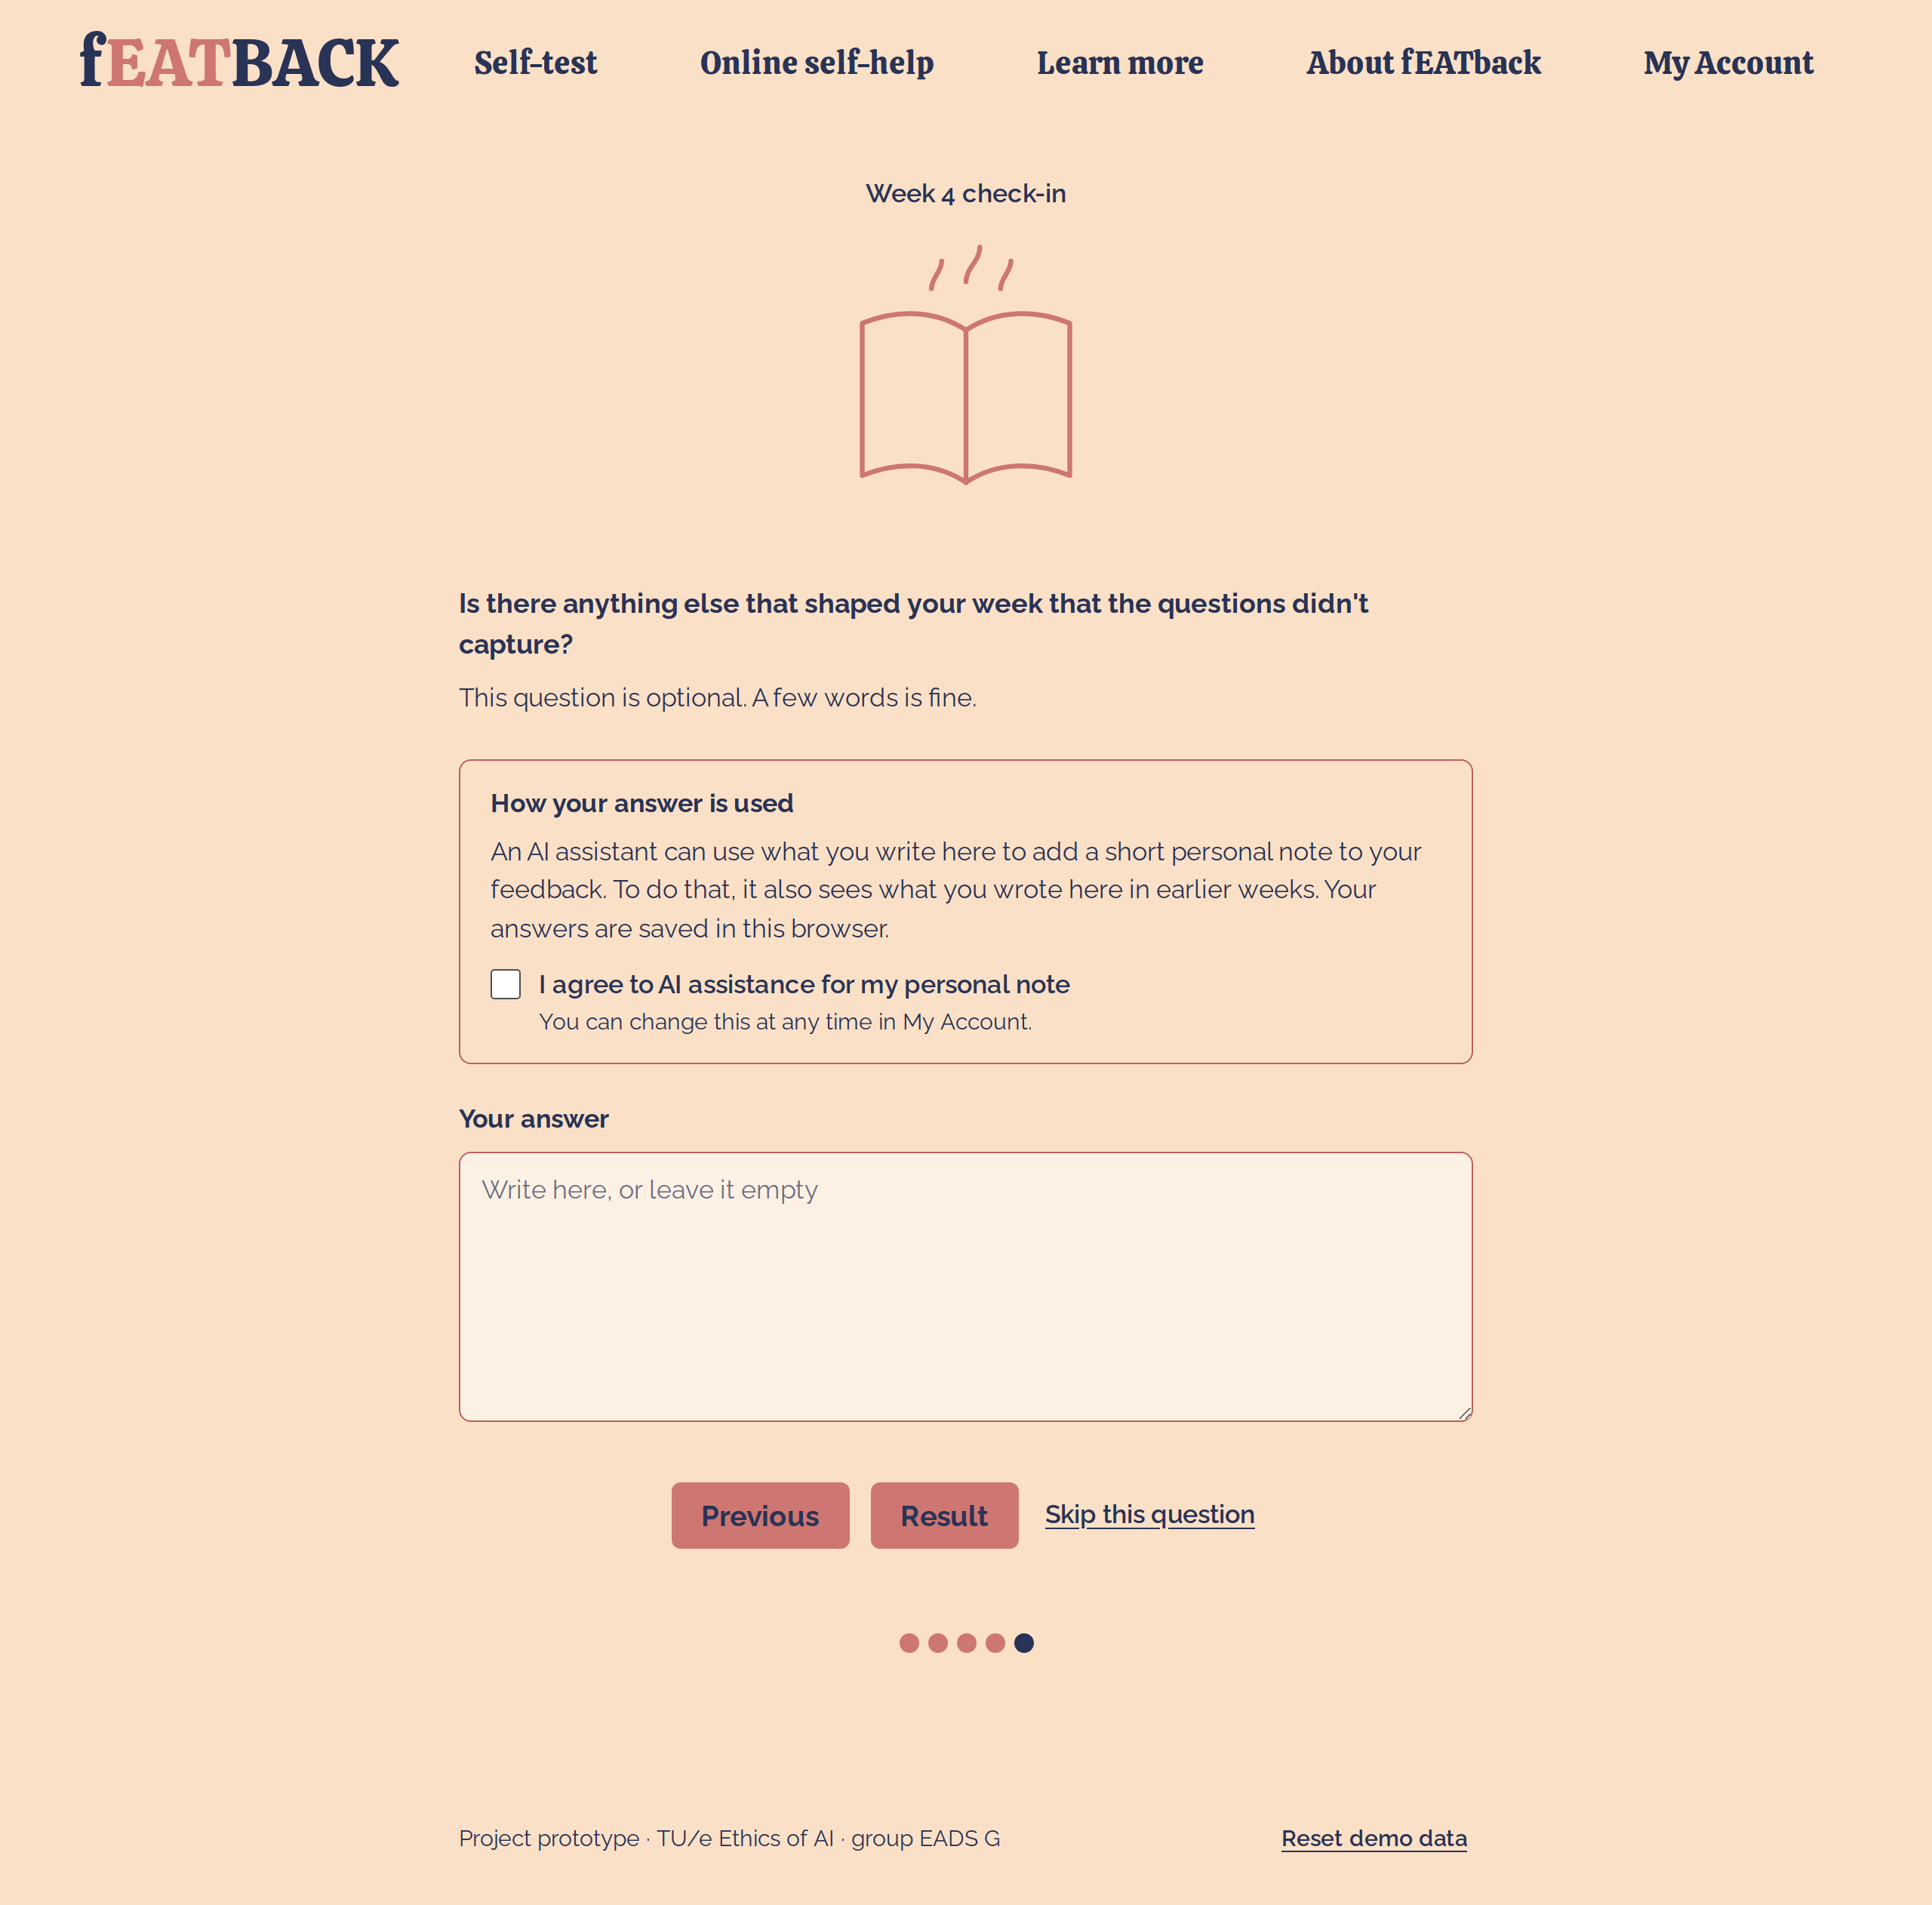
\includegraphics[width=\linewidth, trim=590 1087 590 760, clip]{q5_unticked.png}};
  \begin{scope}[x={(s.south east)}, y={(s.north west)}]
    \callout{0.979}{0.637}{1}
  \end{scope}
\end{tikzpicture}
\par\vspace{4mm}
\paneltitle{b}{Her answer and the result}
\begin{tikzpicture}
  \node[shot] (s) at (0,0) {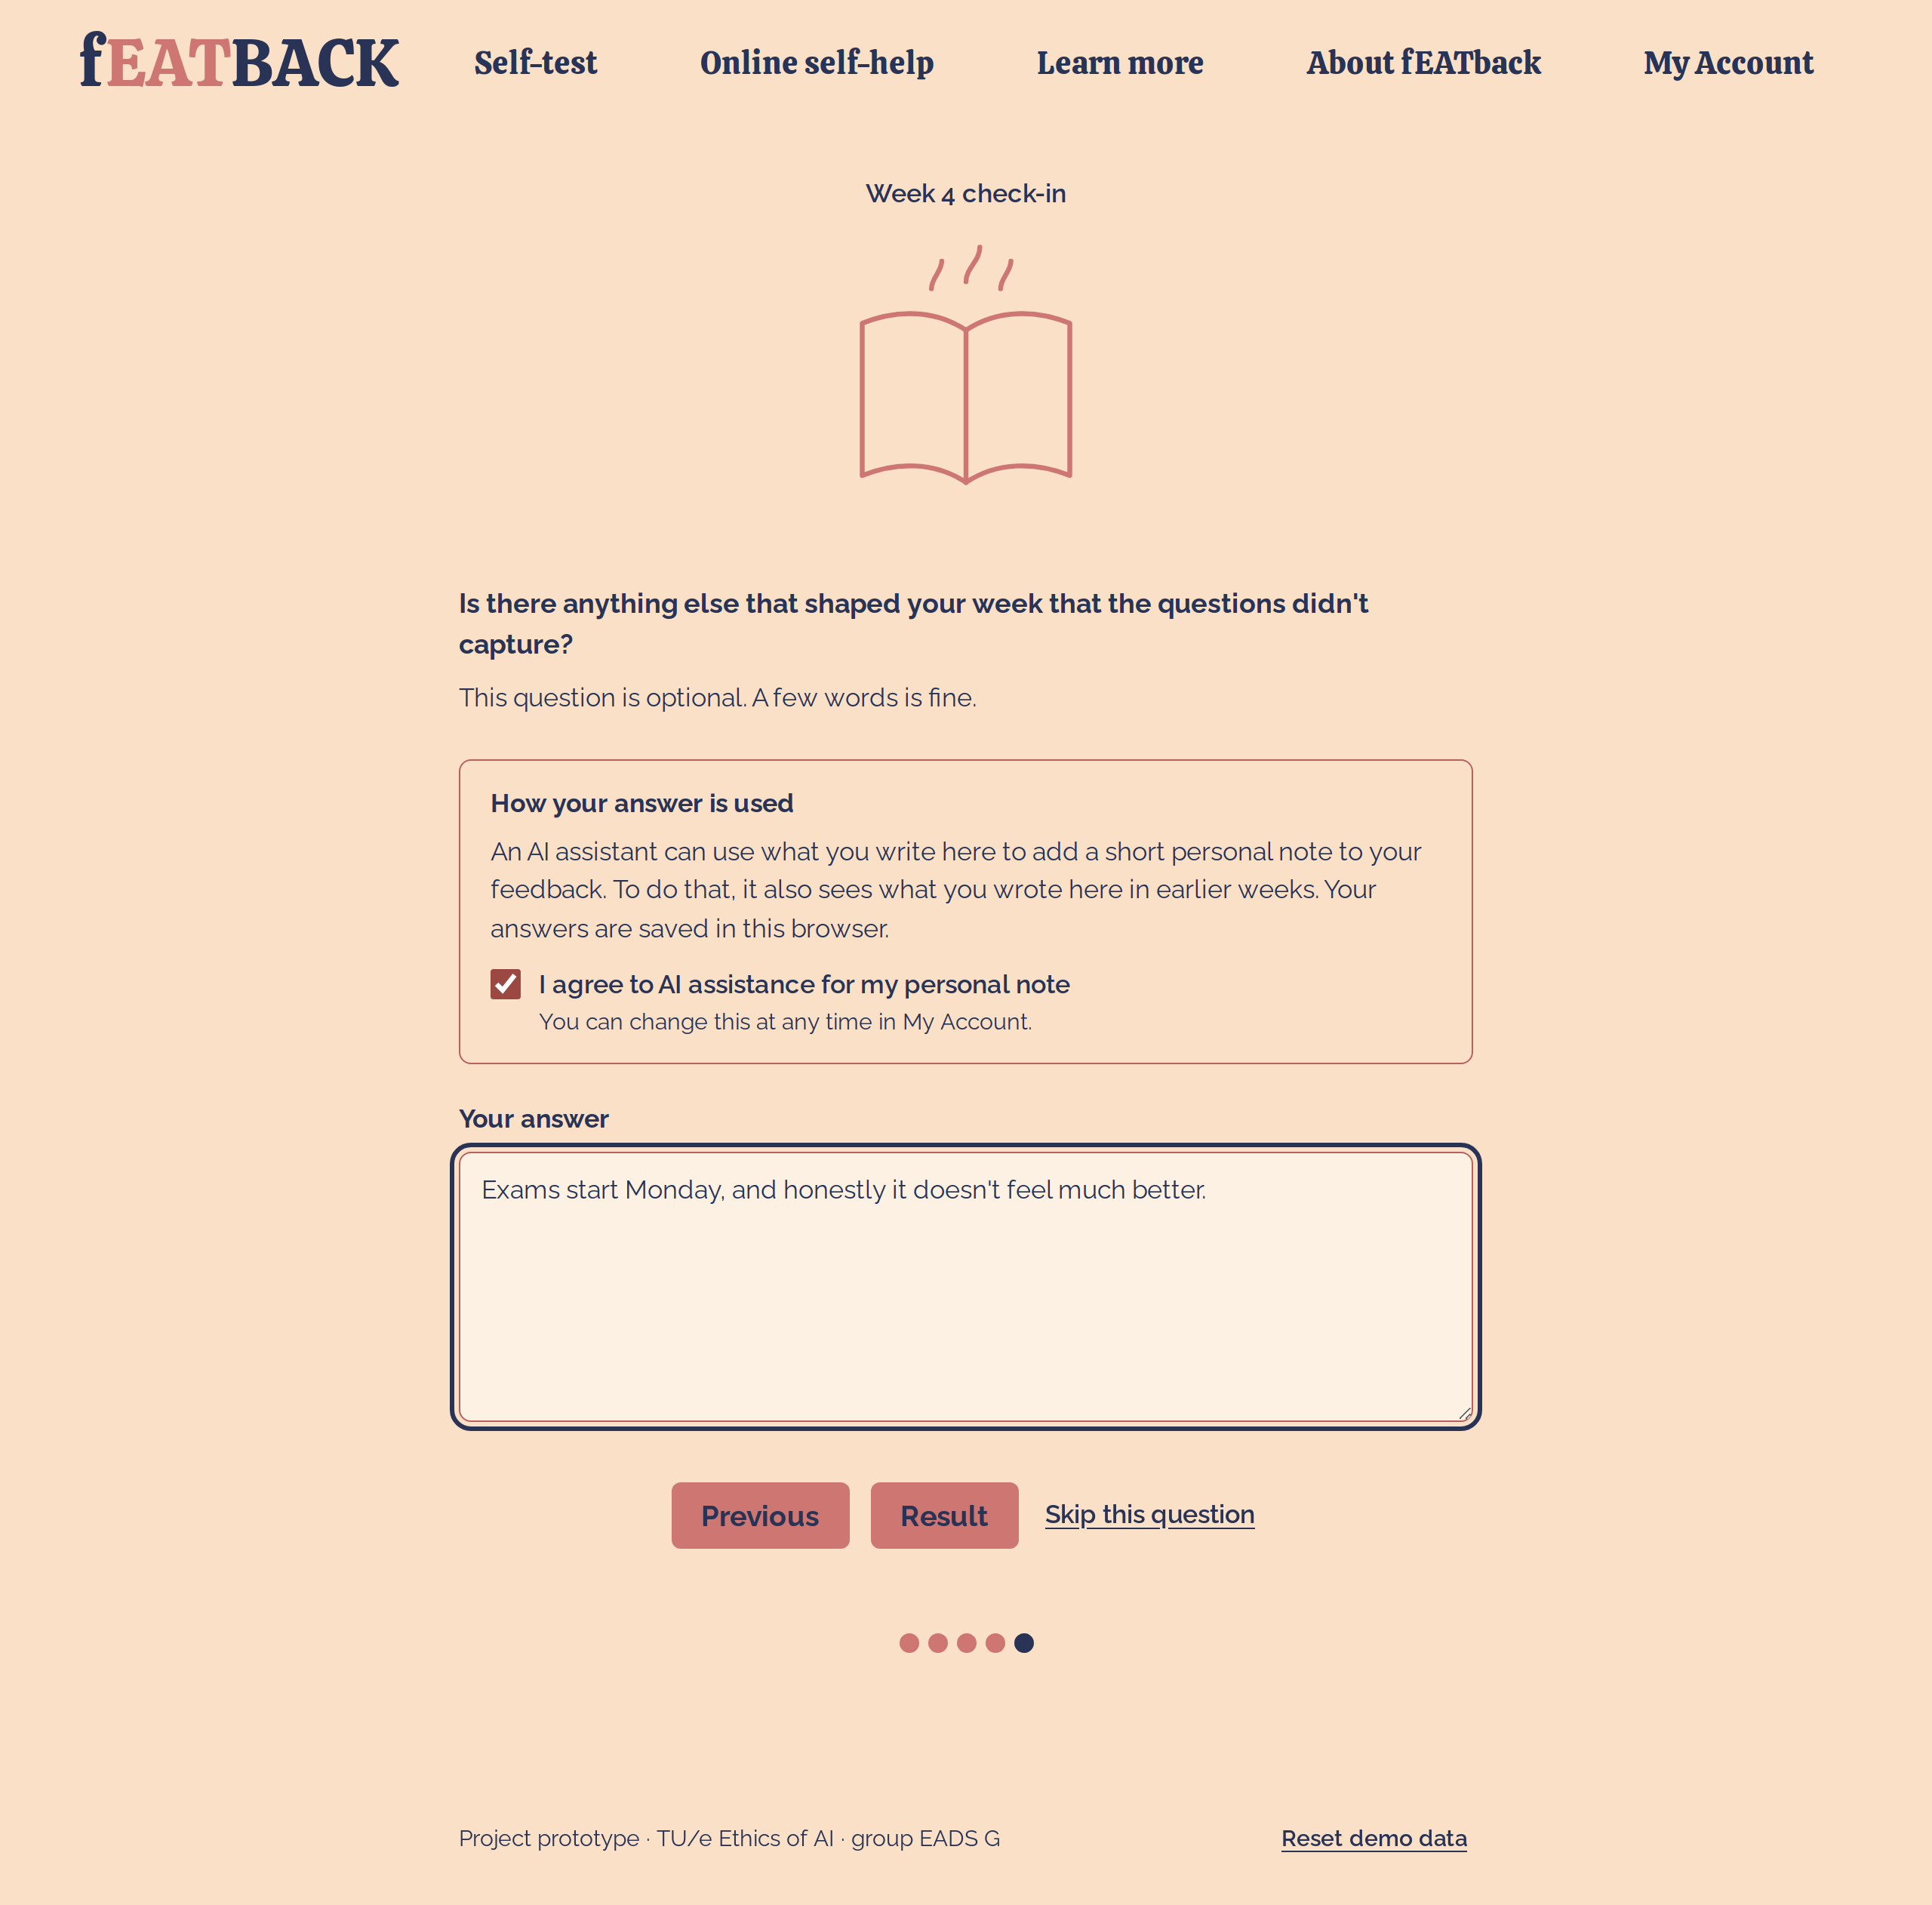
\includegraphics[width=\linewidth, trim=590 613 590 1440, clip]{q5_screen.png}};
  \begin{scope}[x={(s.south east)}, y={(s.north west)}]
    \callout{0.979}{0.817}{2}
  \end{scope}
\end{tikzpicture}
\par\vspace{1.5mm}
\begin{tikzpicture}
  \node[shot] (s) at (0,0) {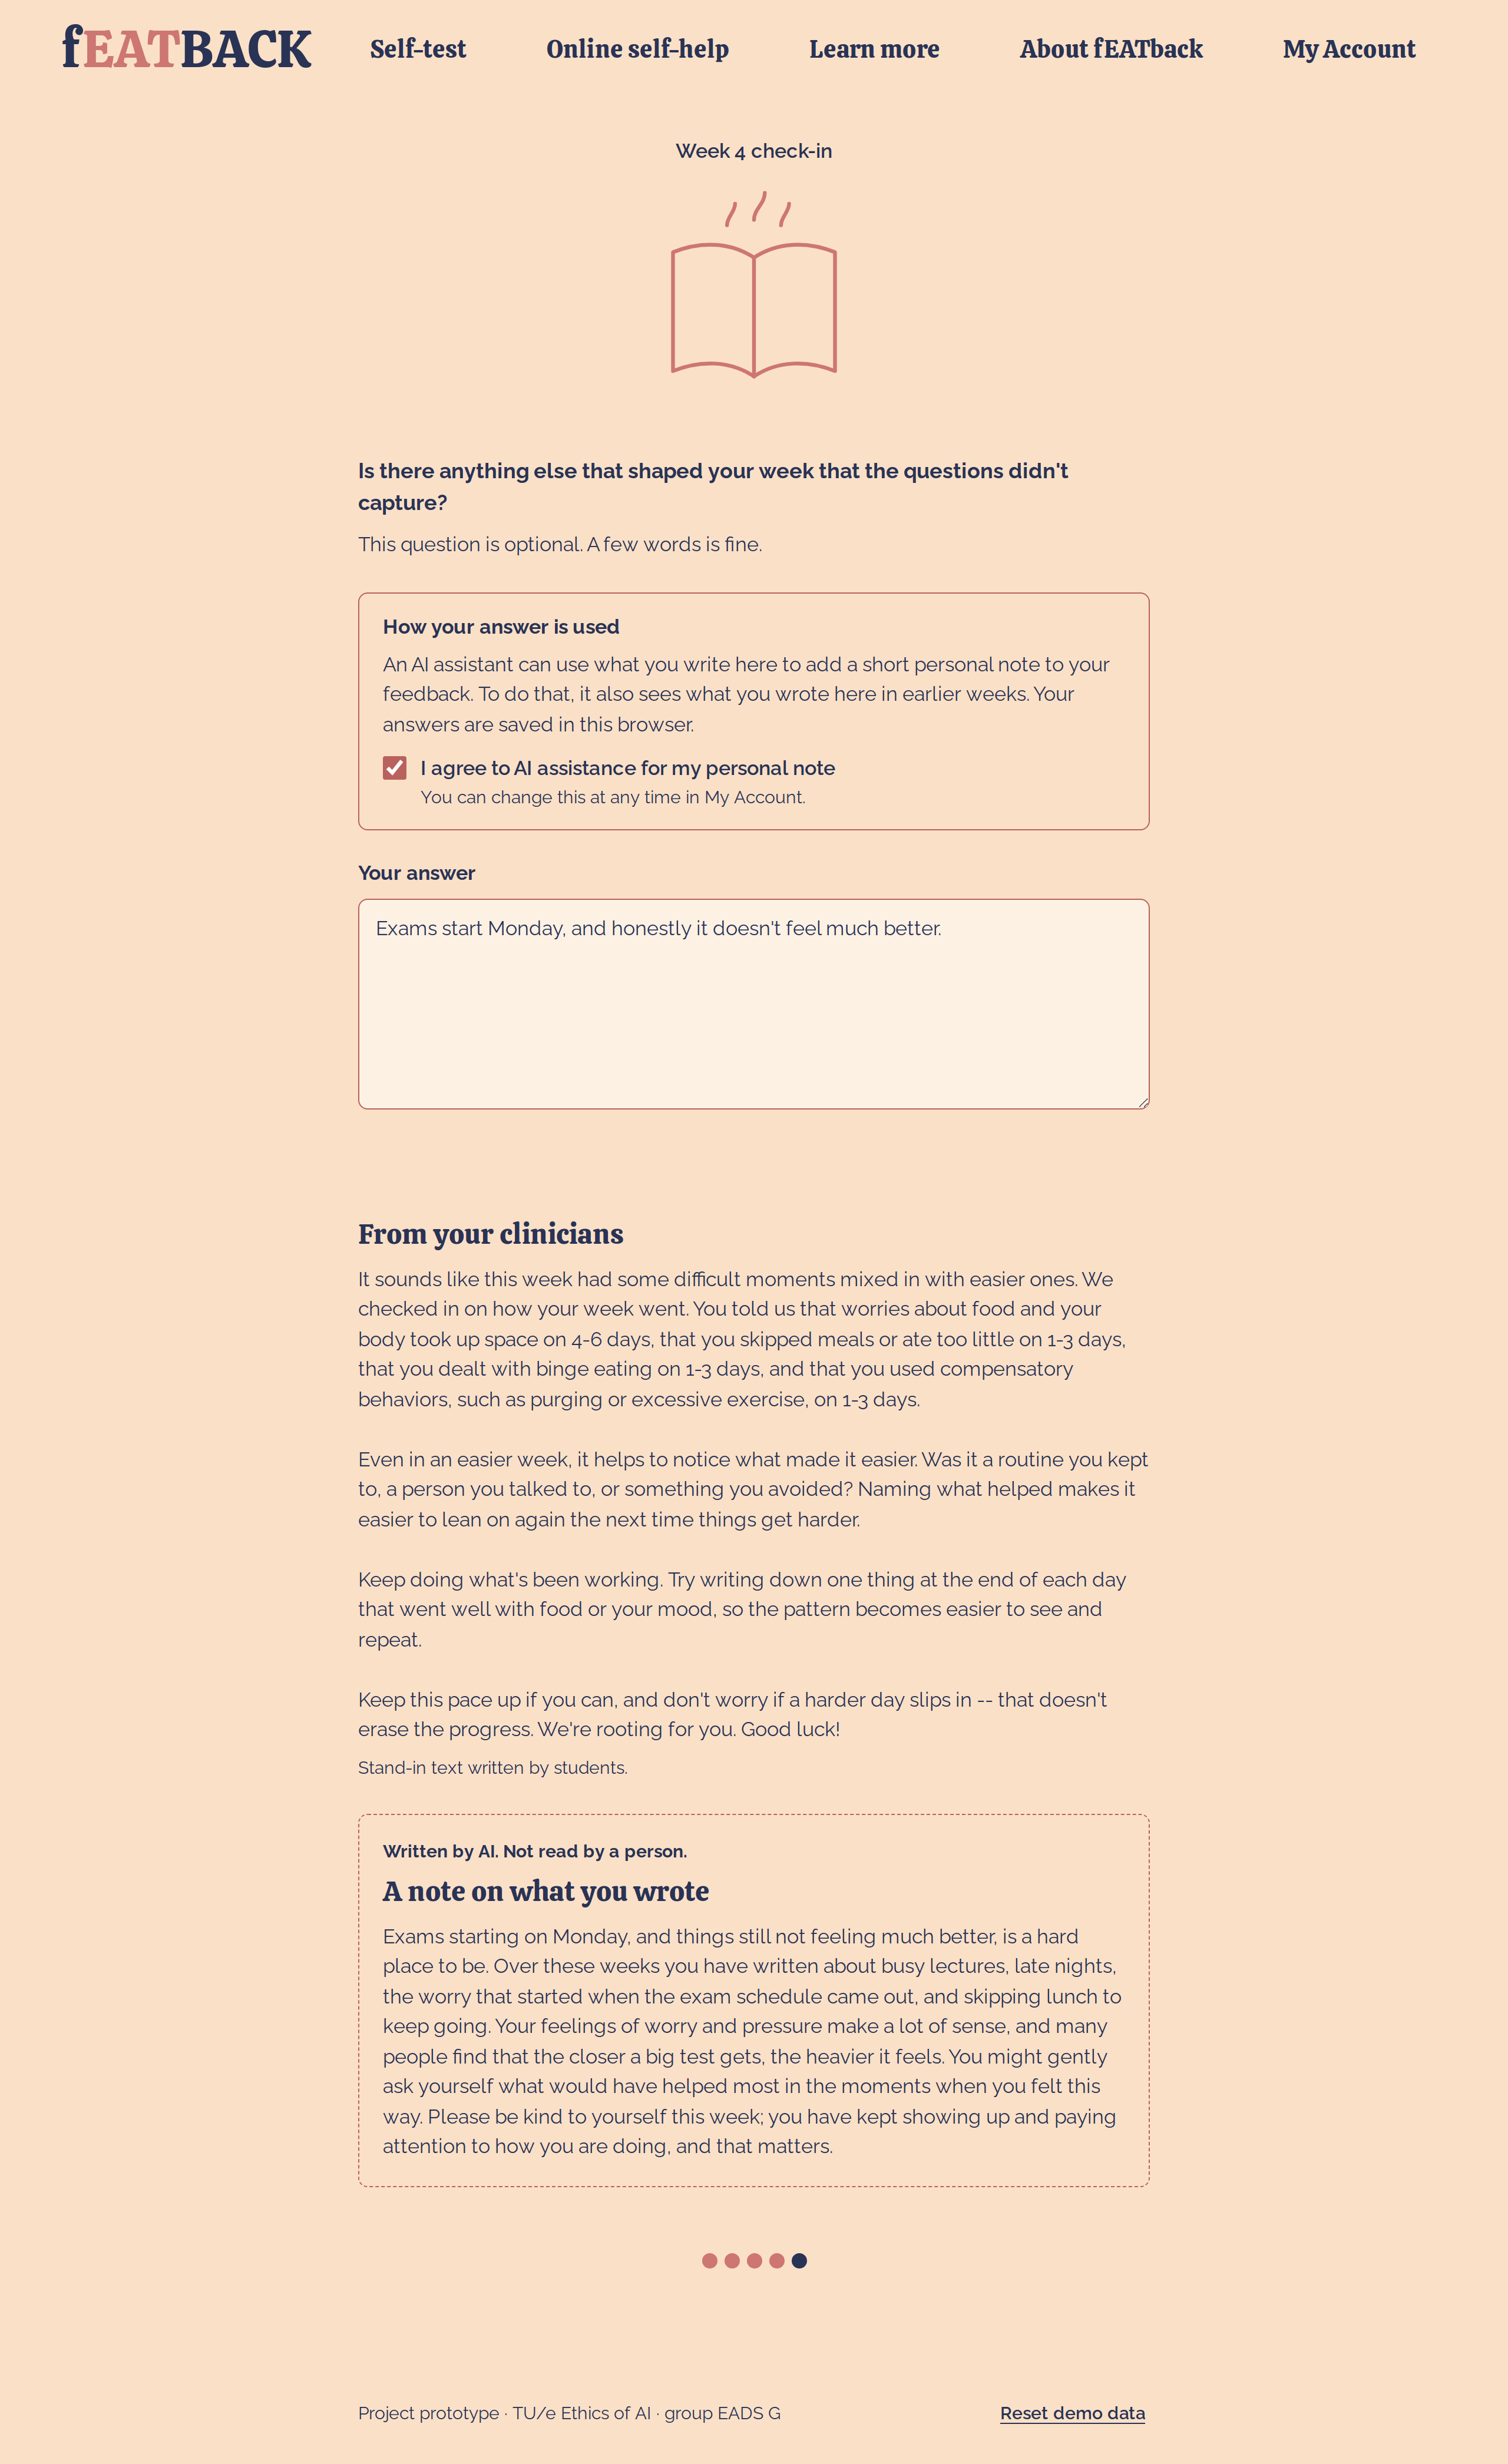
\includegraphics[width=\linewidth, trim=590 443 590 2046, clip]{result_screen.png}};
  \begin{scope}[x={(s.south east)}, y={(s.north west)}]
    \callout{0.979}{0.983}{3}
    \callout{0.979}{0.390}{4}
  \end{scope}
\end{tikzpicture}
\end{minipage}%
\hfill
% ============ Right column: other weeks and edge cases ============
\begin{minipage}[t]{0.47\textwidth}
\colhead{Week 5 and when something goes wrong}
\paneltitle{c}{Week 5, where the note looks back}
\begin{tikzpicture}
  \node[shot] (s) at (0,0) {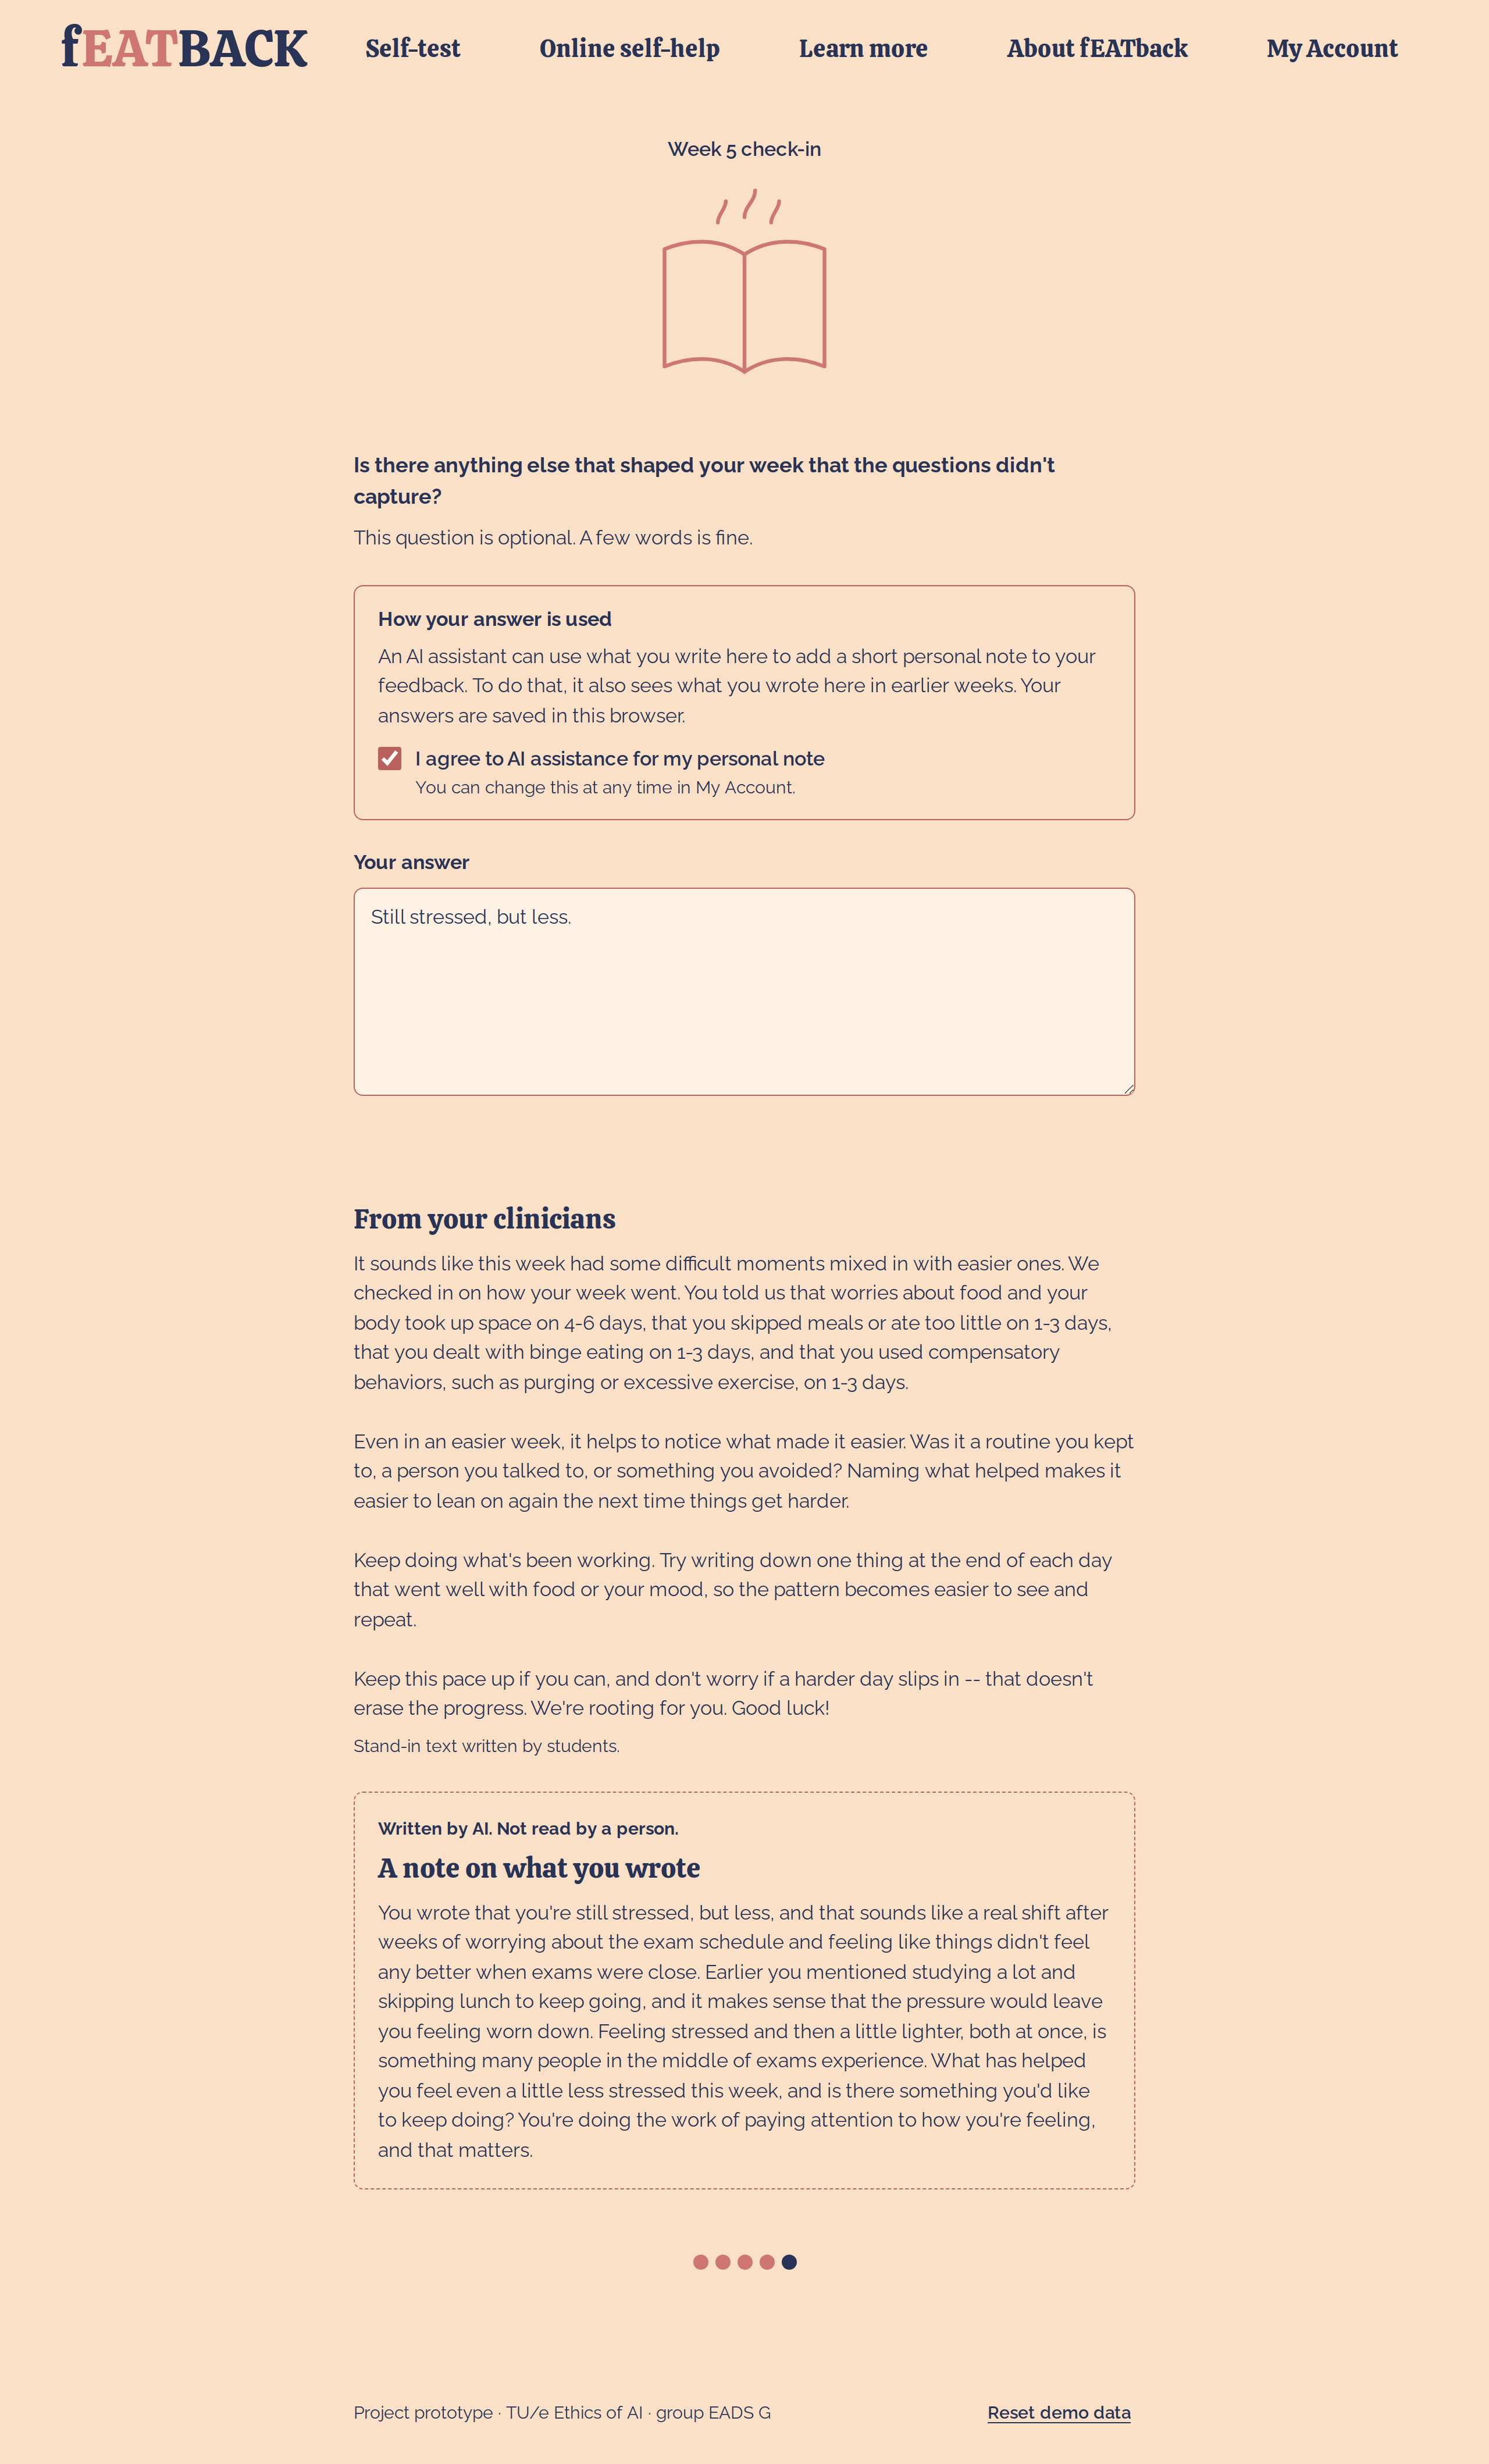
\includegraphics[width=\linewidth, trim=590 2325 590 1440, clip]{result_week5.png}};
\end{tikzpicture}
\par\vspace{1.5mm}
\begin{tikzpicture}
  \node[shot] (s) at (0,0) {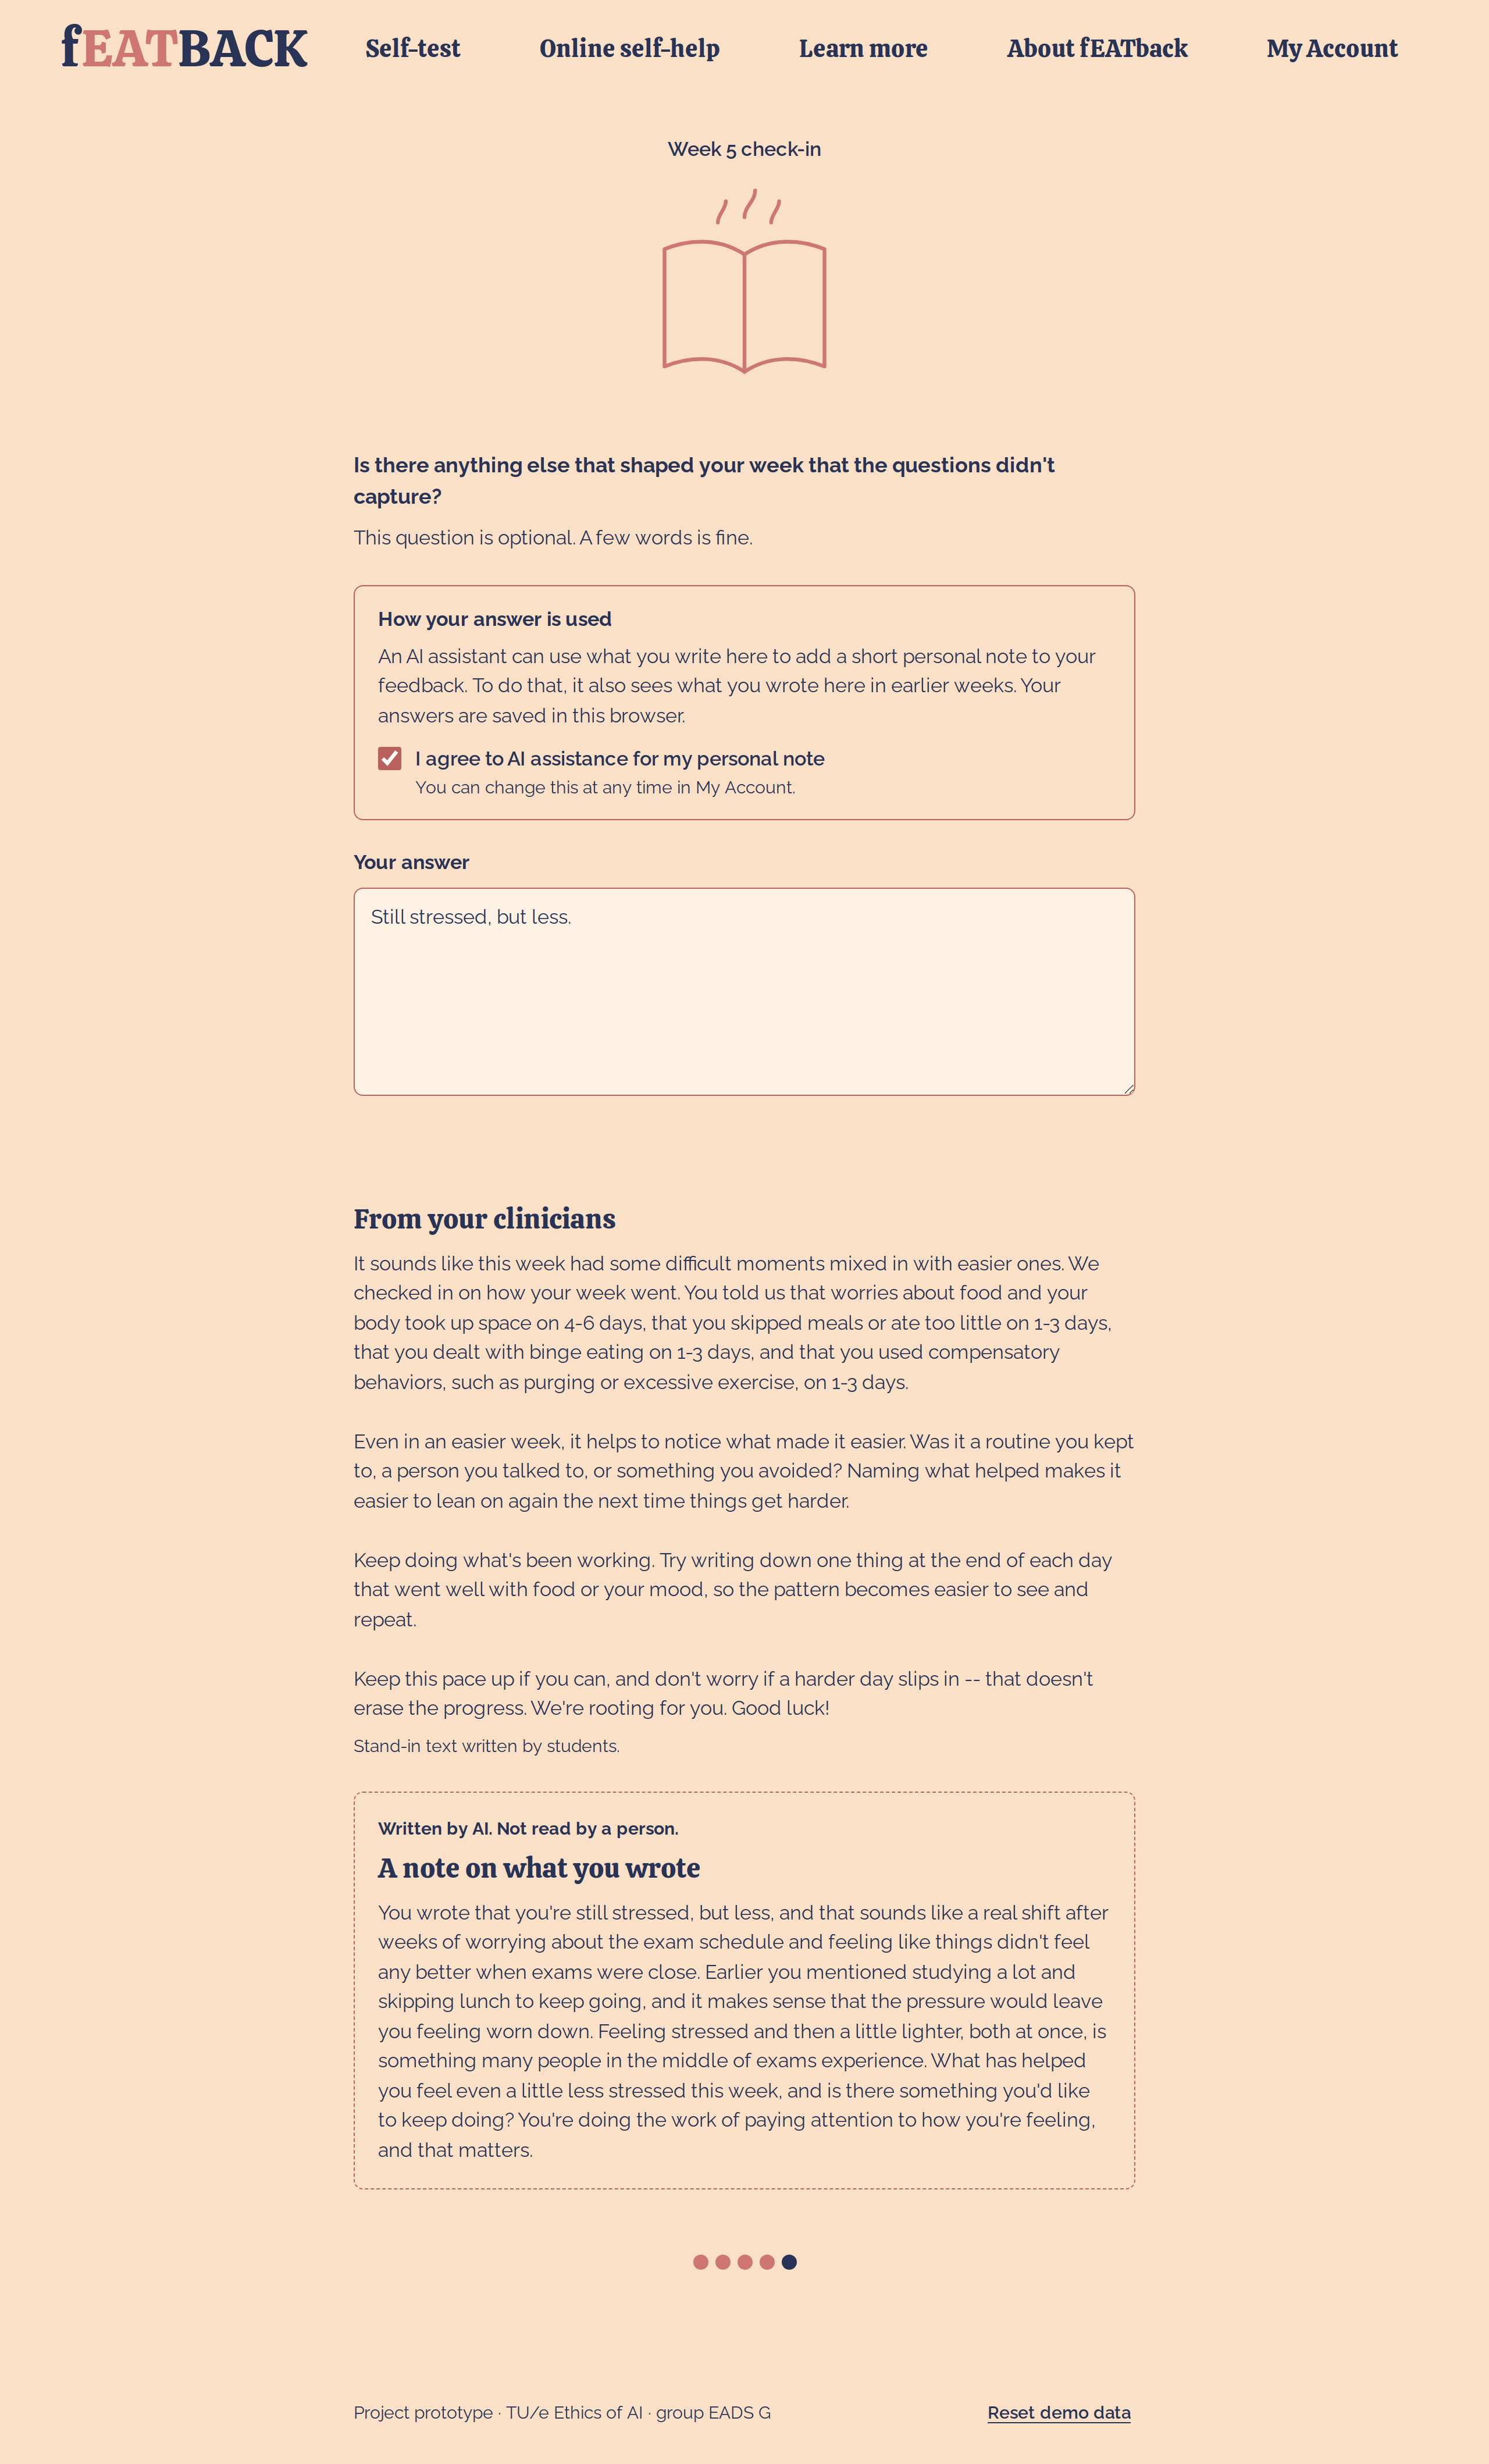
\includegraphics[width=\linewidth, trim=590 445 590 3052, clip]{result_week5.png}};
\end{tikzpicture}
\par\vspace{4mm}
\paneltitle{d}{Model off or note rejected}
\begin{tikzpicture}
  \node[shot] (s) at (0,0) {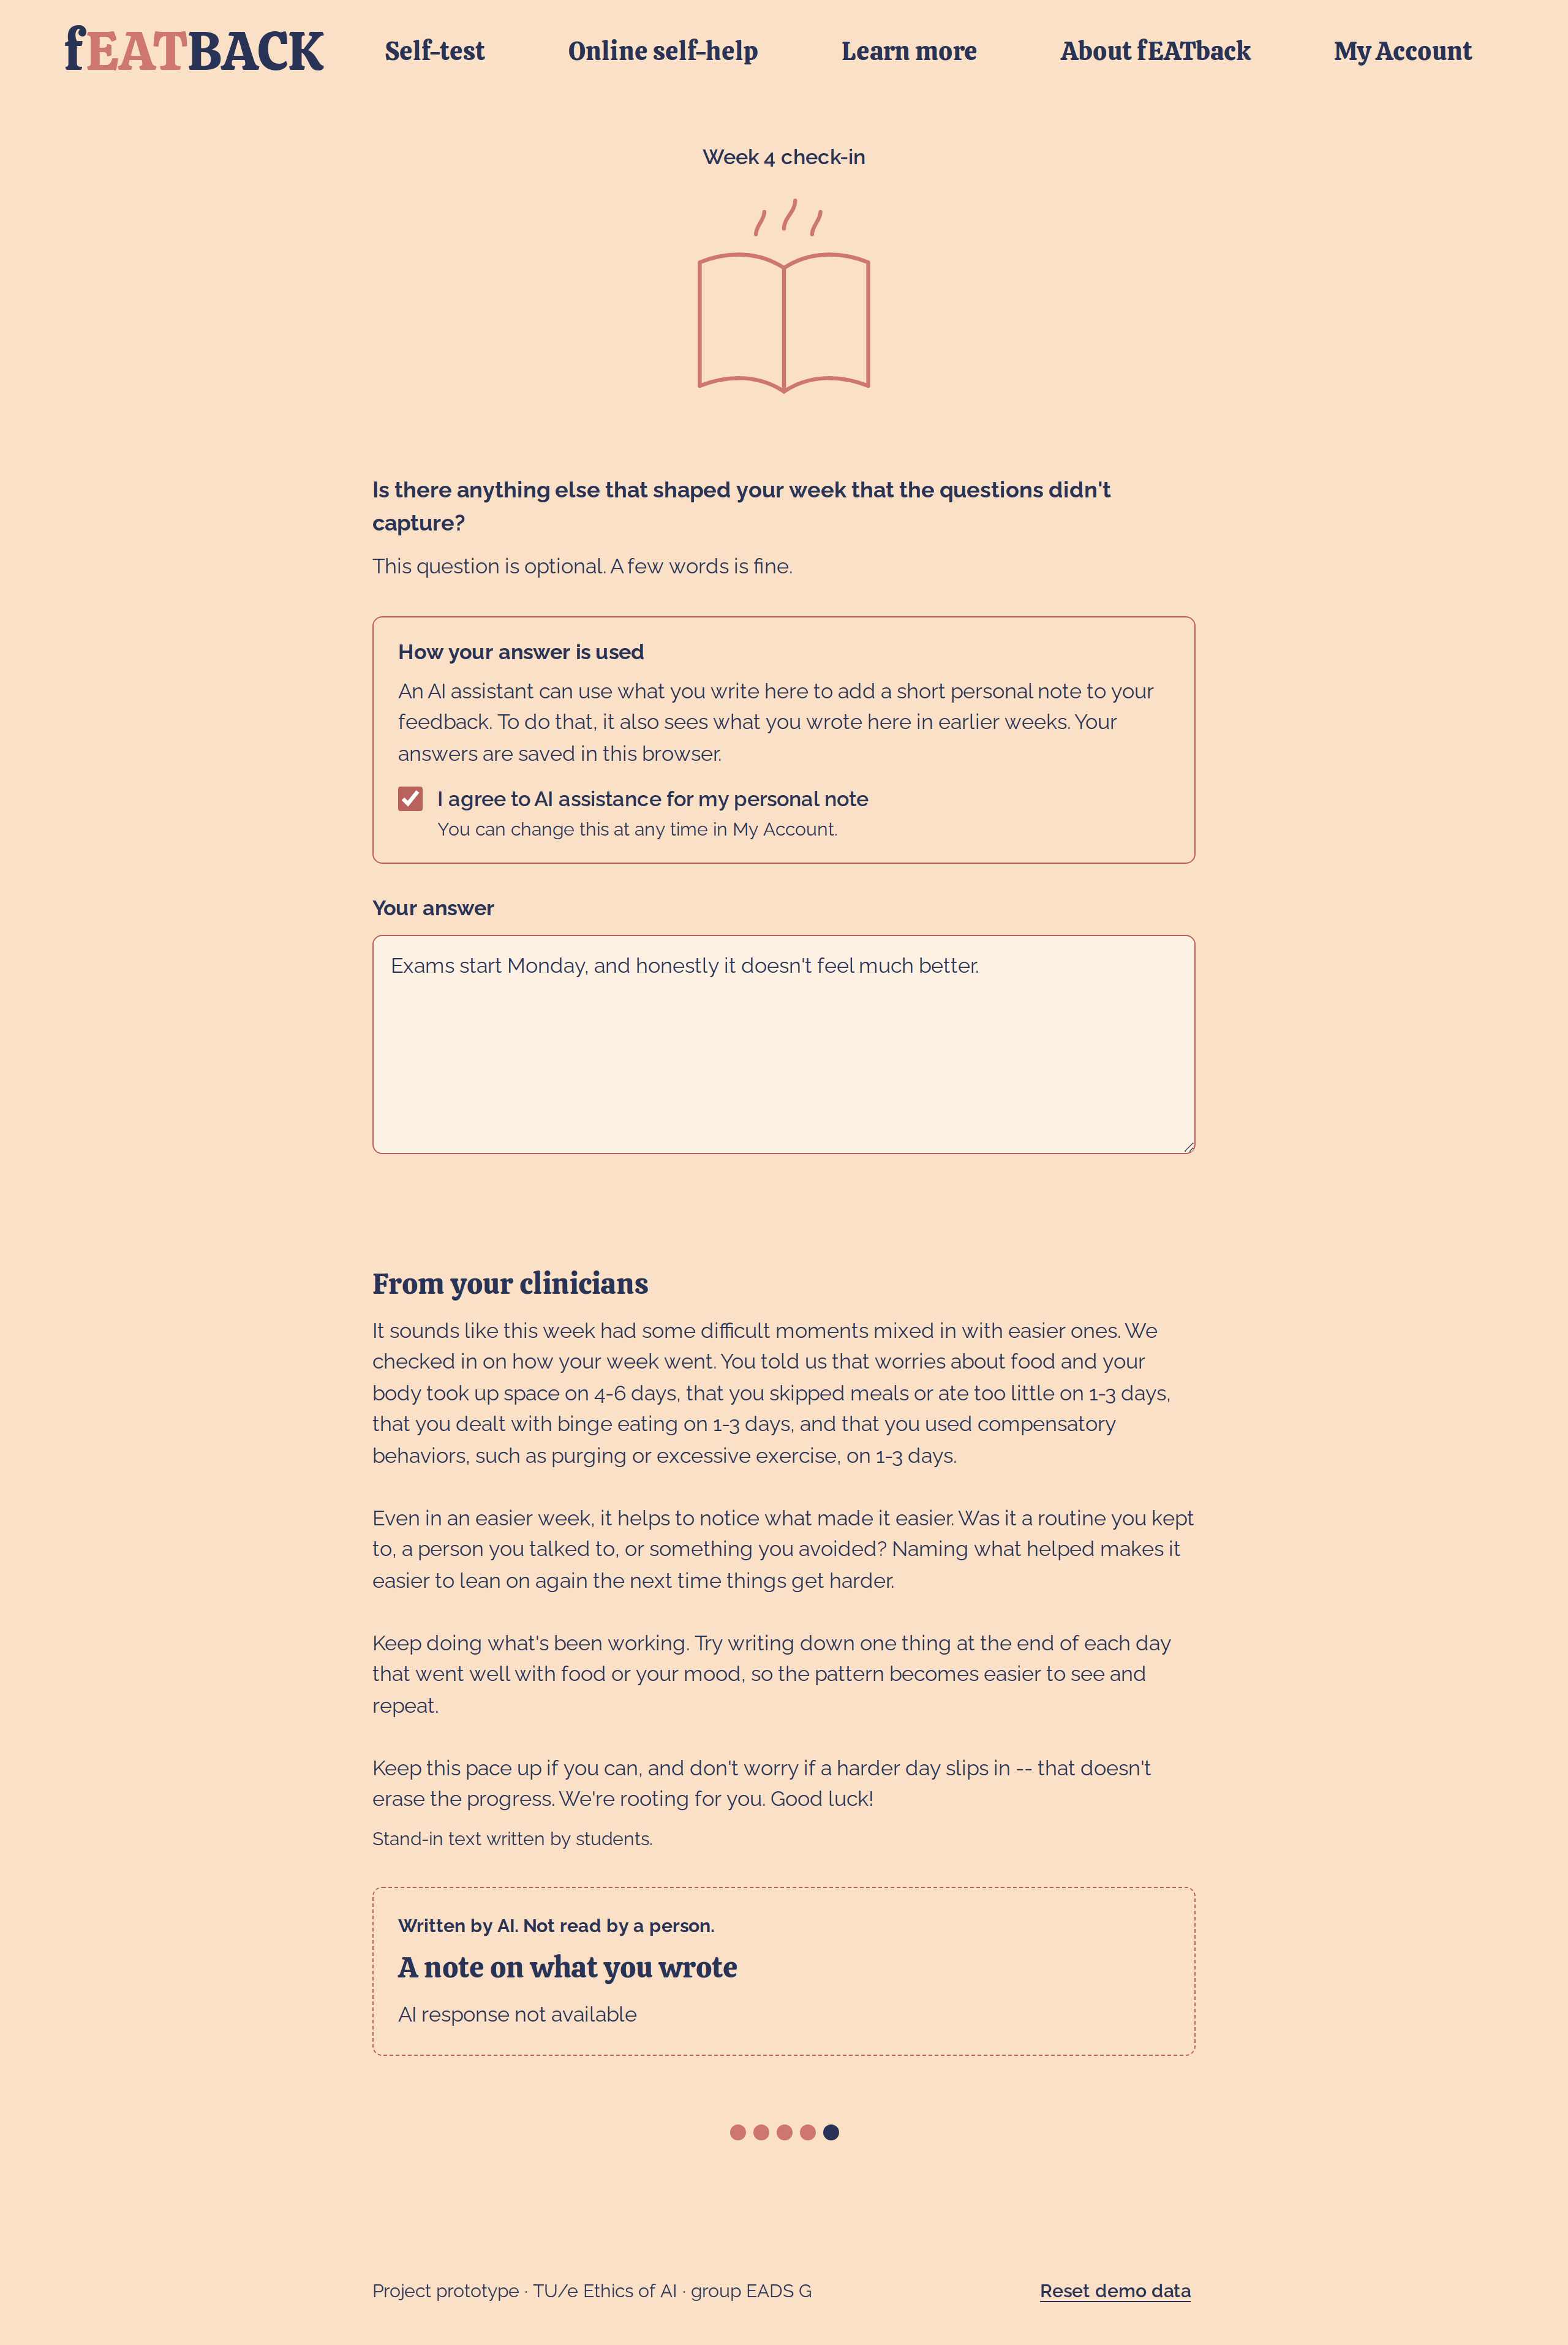
\includegraphics[width=\linewidth, trim=590 445 590 3052, clip]{fallback.png}};
  \begin{scope}[x={(s.south east)}, y={(s.north west)}]
    \callout{0.979}{0.915}{5}
  \end{scope}
\end{tikzpicture}
\par\vspace{4mm}
\paneltitle{e}{An answer with signs of acute risk}
\begin{tikzpicture}
  \node[shot] (s) at (0,0) {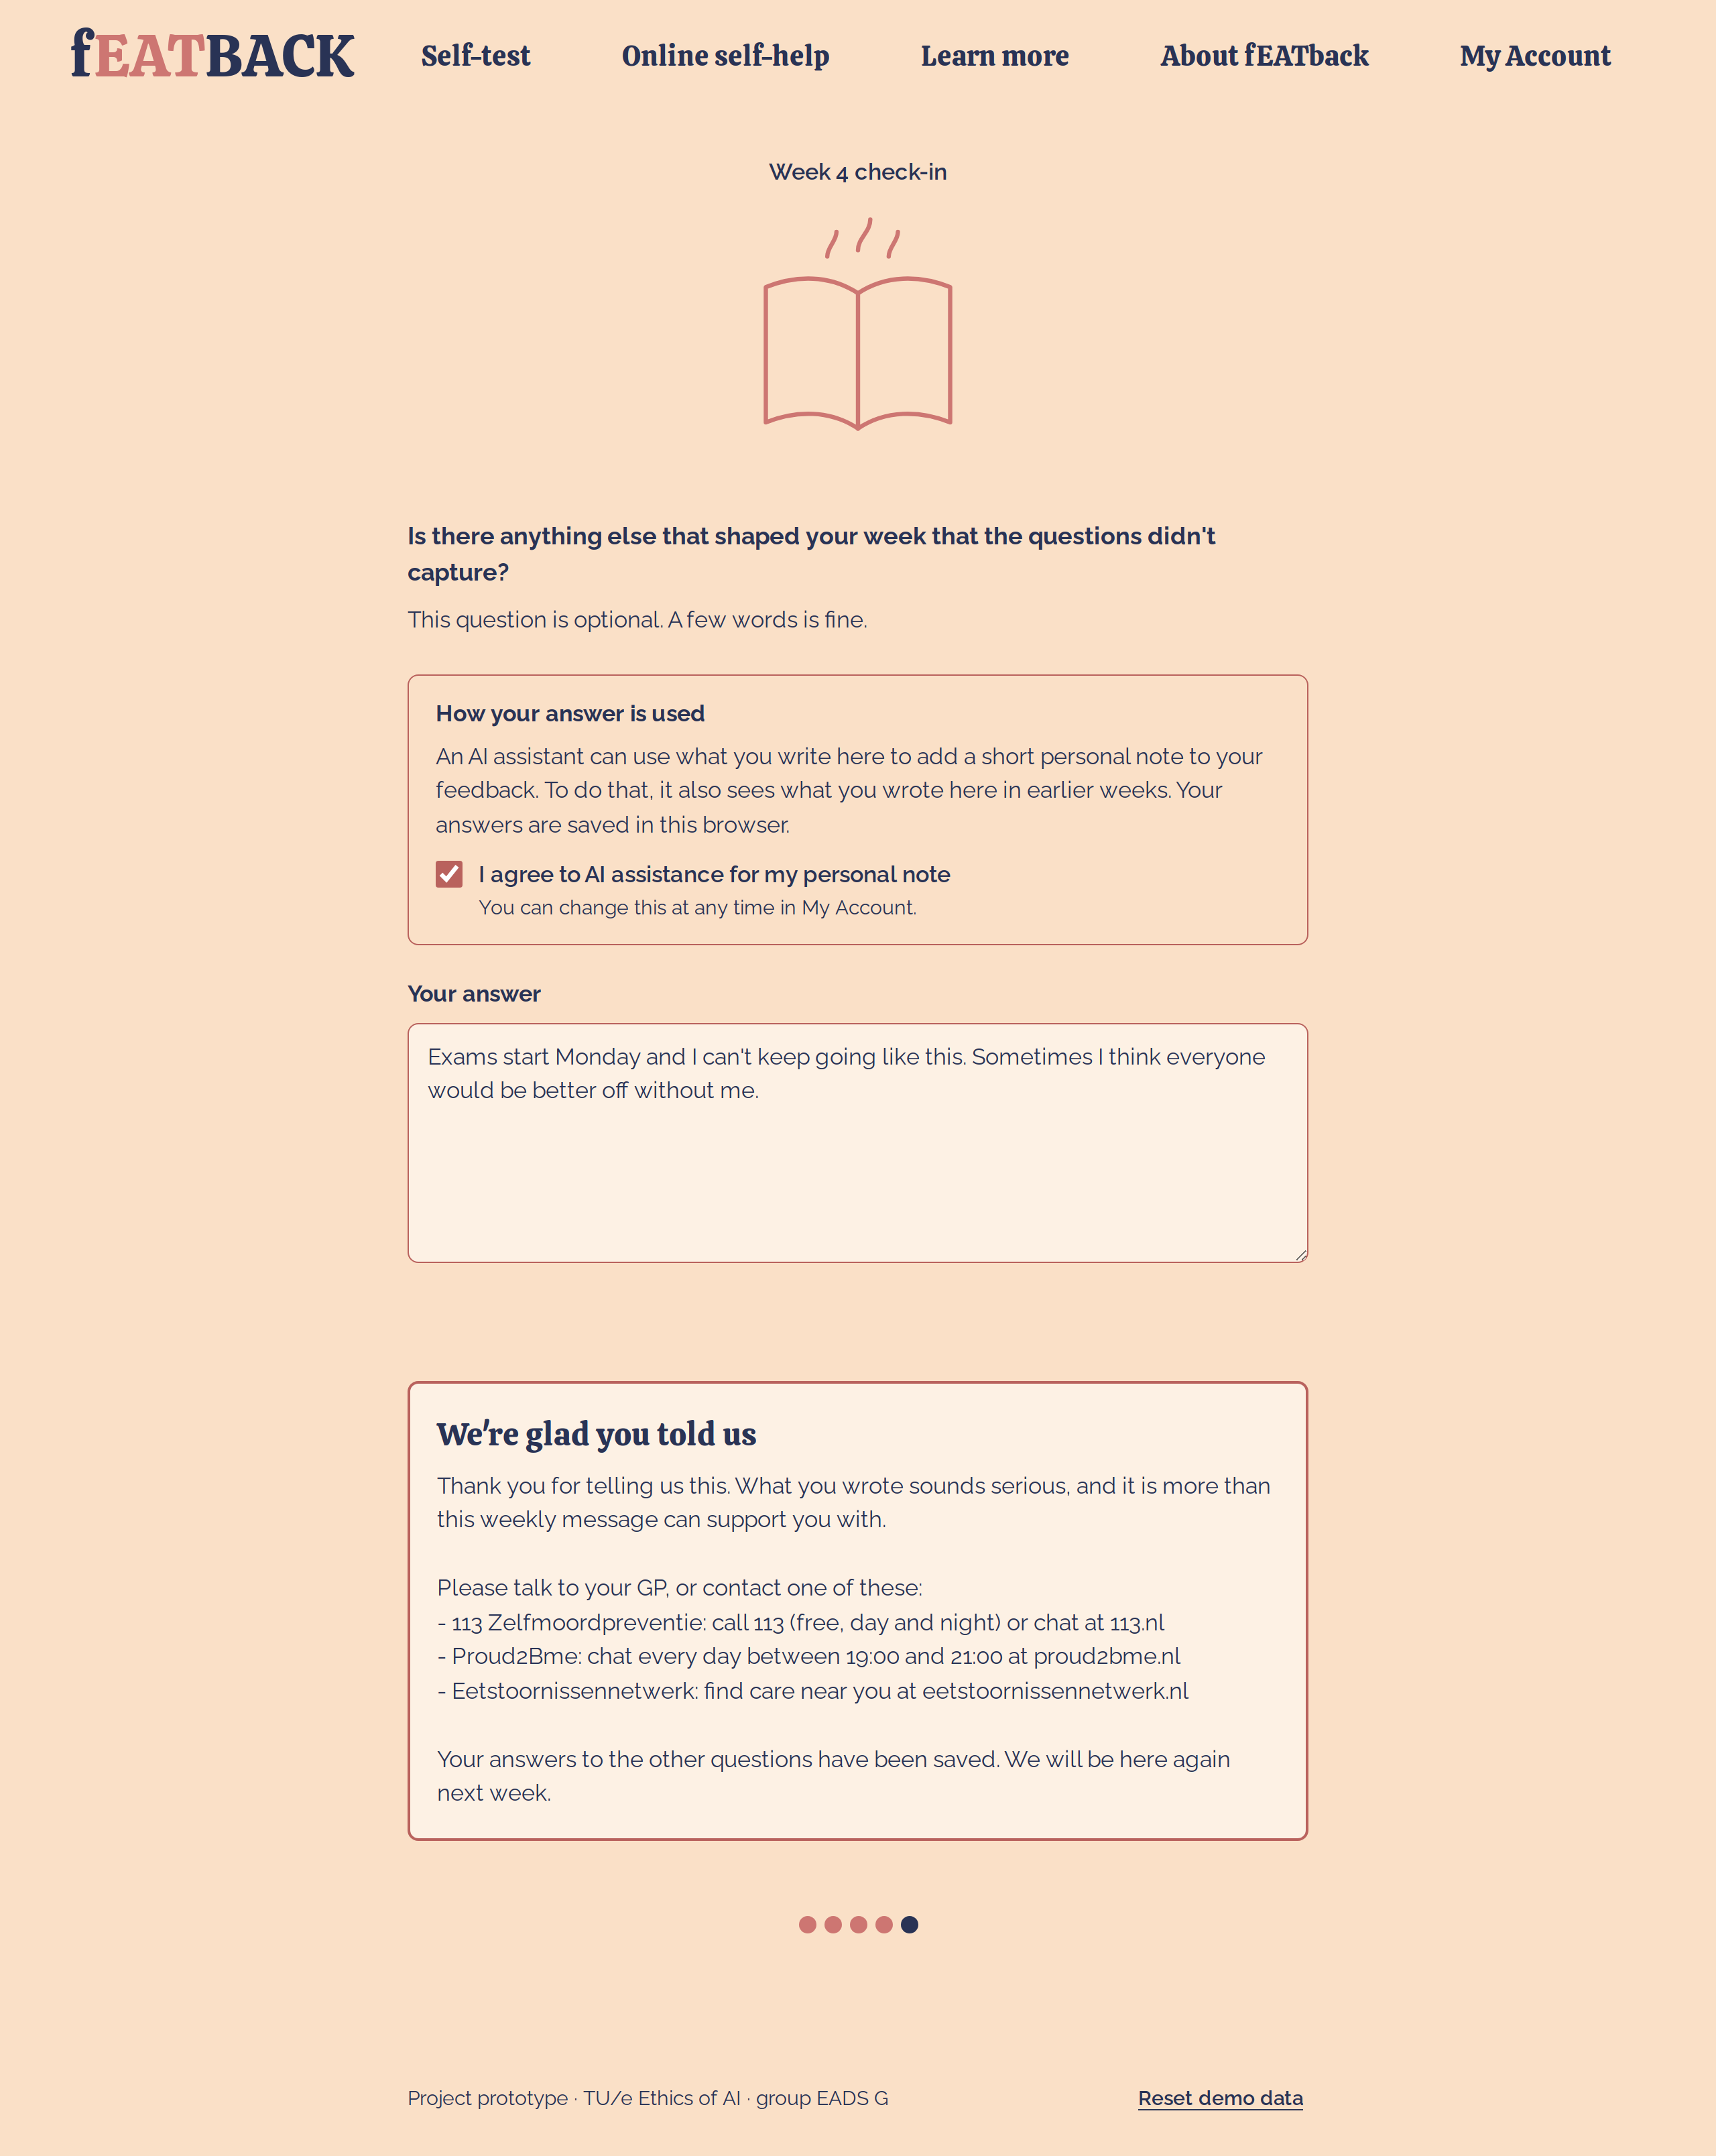
\includegraphics[width=\linewidth, trim=590 1305 590 1440, clip]{acute.png}};
\end{tikzpicture}
\par\vspace{1.5mm}
\begin{tikzpicture}
  \node[shot] (s) at (0,0) {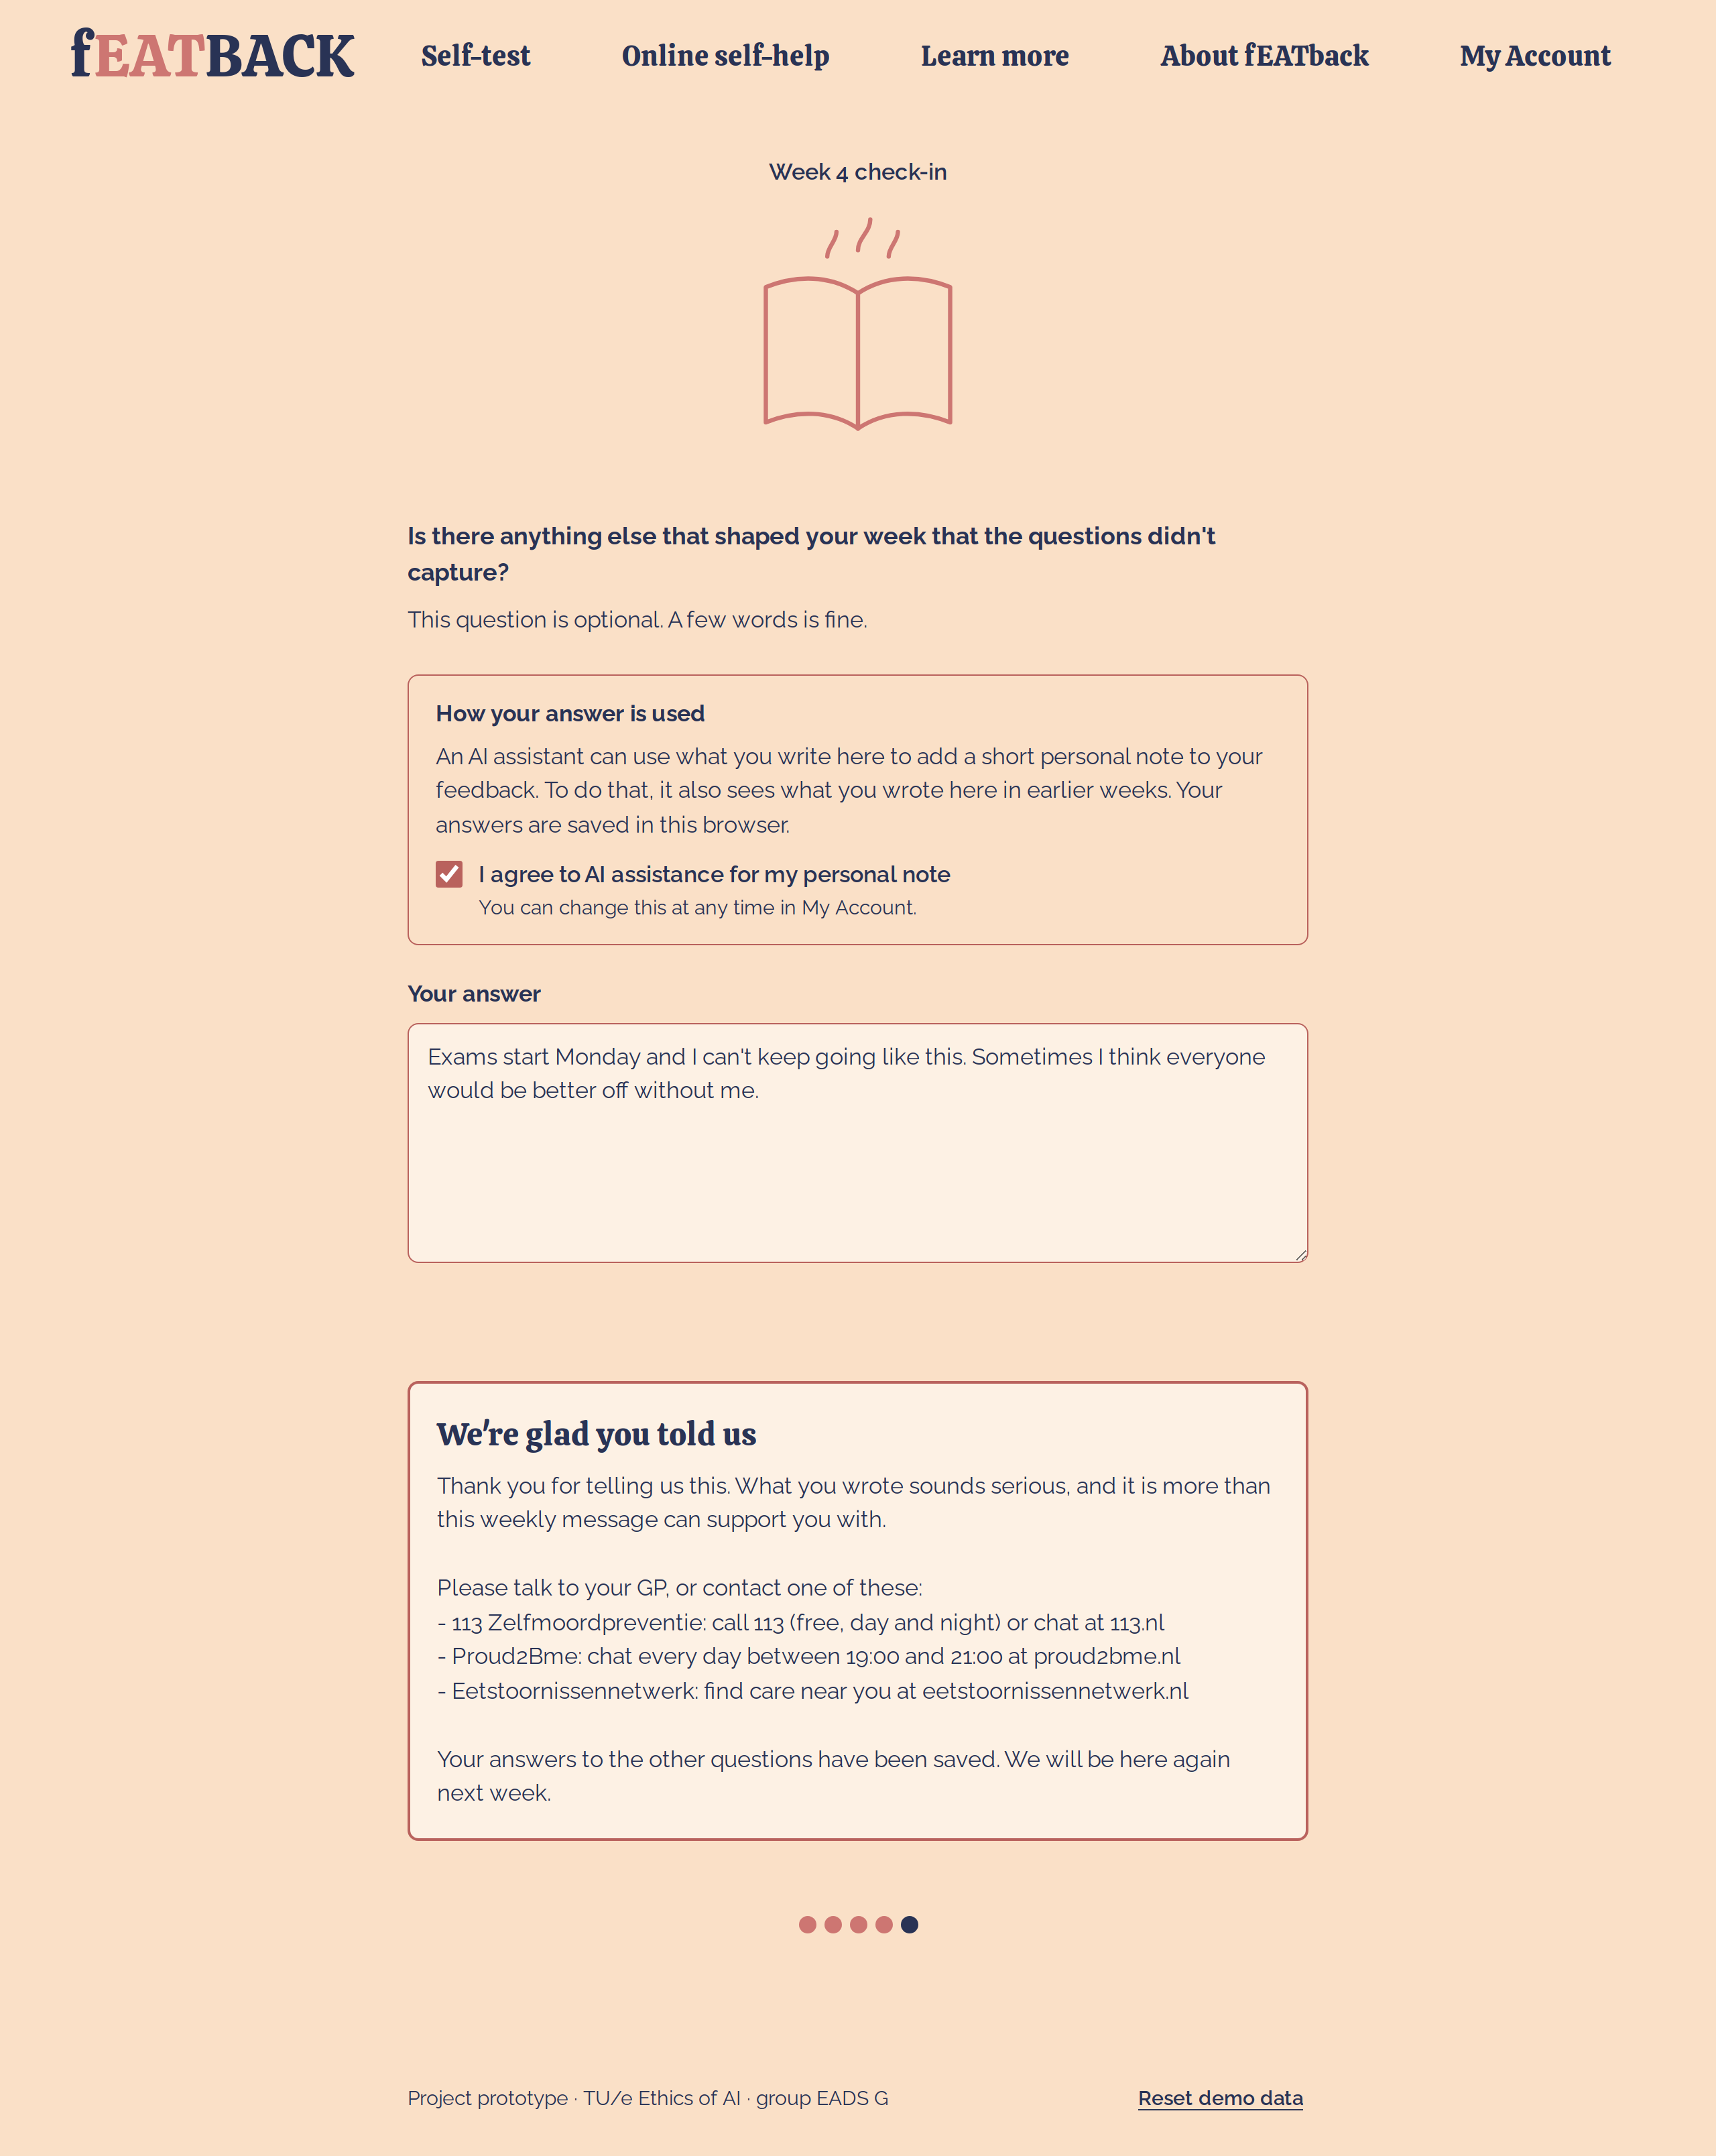
\includegraphics[width=\linewidth, trim=590 443 590 2032, clip]{acute.png}};
  \begin{scope}[x={(s.south east)}, y={(s.north west)}]
    \callout{0.979}{0.962}{6}
  \end{scope}
\end{tikzpicture}
\end{minipage}

\vspace{5mm}
% ---- Key: one entry per callout, aligned with the two columns ----
\newcommand{\keyline}[2]{\key{#1}\hspace{2mm}#2\par\vspace{1.2mm}}
{\footnotesize\sffamily
\begin{minipage}[t]{0.47\textwidth}
\keyline{1}{Consent box starts unticked (part 3)}
\keyline{2}{Answer stored for the trend (part 3)}
\keyline{3}{Stand-in bank message (part 1)}
\end{minipage}\hfill
\begin{minipage}[t]{0.47\textwidth}
\keyline{4}{Label on every AI note (part 2)}
\keyline{5}{Fixed fallback text we wrote (part 1)}
\keyline{6}{Gate takes the more severe label (part 1)}
\end{minipage}}

\vspace{2mm}
\caption{Maren's check-ins from Section~\ref{sec:narrative} as they appear on screen. Part numbers in the key
point to the Responsible Innovation statement. The AI notes in (b) and (c) are real
output from our fine-tuned writer model, run on 12 October 2026. The bank message, Maren
and her earlier answers are made up for the demo.}
\label{fig:mockup}
\end{figure}
.
% Needs tikz (loaded by todonotes in main.tex), graphicx and float.

% ---- Figure style ----------------------------------------------------------
\definecolor{fbnavy}{HTML}{283357}
\tikzset{
  shot/.style={anchor=south west, inner sep=0, draw=black!18, line width=0.4pt},
  callout/.style={circle, fill=fbnavy, draw=white, line width=0.9pt, text=white,
    font=\sffamily\bfseries\scriptsize, inner sep=0pt, minimum size=4.4mm}}
% Callouts sit on the right edge, level with the element they mark.
\newcommand{\callout}[3]{\node[callout, overlay] at (#1,#2) {#3};}
% Inline callout for the key
\newcommand{\key}[1]{\tikz[baseline=-0.6ex]\node[callout]{#1};}
% Panel title
\newcommand{\paneltitle}[2]{{\sffamily\footnotesize\color{fbnavy}\textbf{(#1)}~#2}\par\vspace{1mm}}
\newcommand{\colhead}[1]{{\sffamily\small\bfseries\color{fbnavy}#1}\par\vspace{0.5mm}{\color{black!25}\hrule height 0.4pt}\vspace{2mm}}

\begin{figure}[H]
\centering
% ============ Left column: week 4 ============
\begin{minipage}[t]{0.47\textwidth}
\colhead{Week 4}
\paneltitle{a}{Question 5, before she agrees}
\begin{tikzpicture}
  \node[shot] (s) at (0,0) {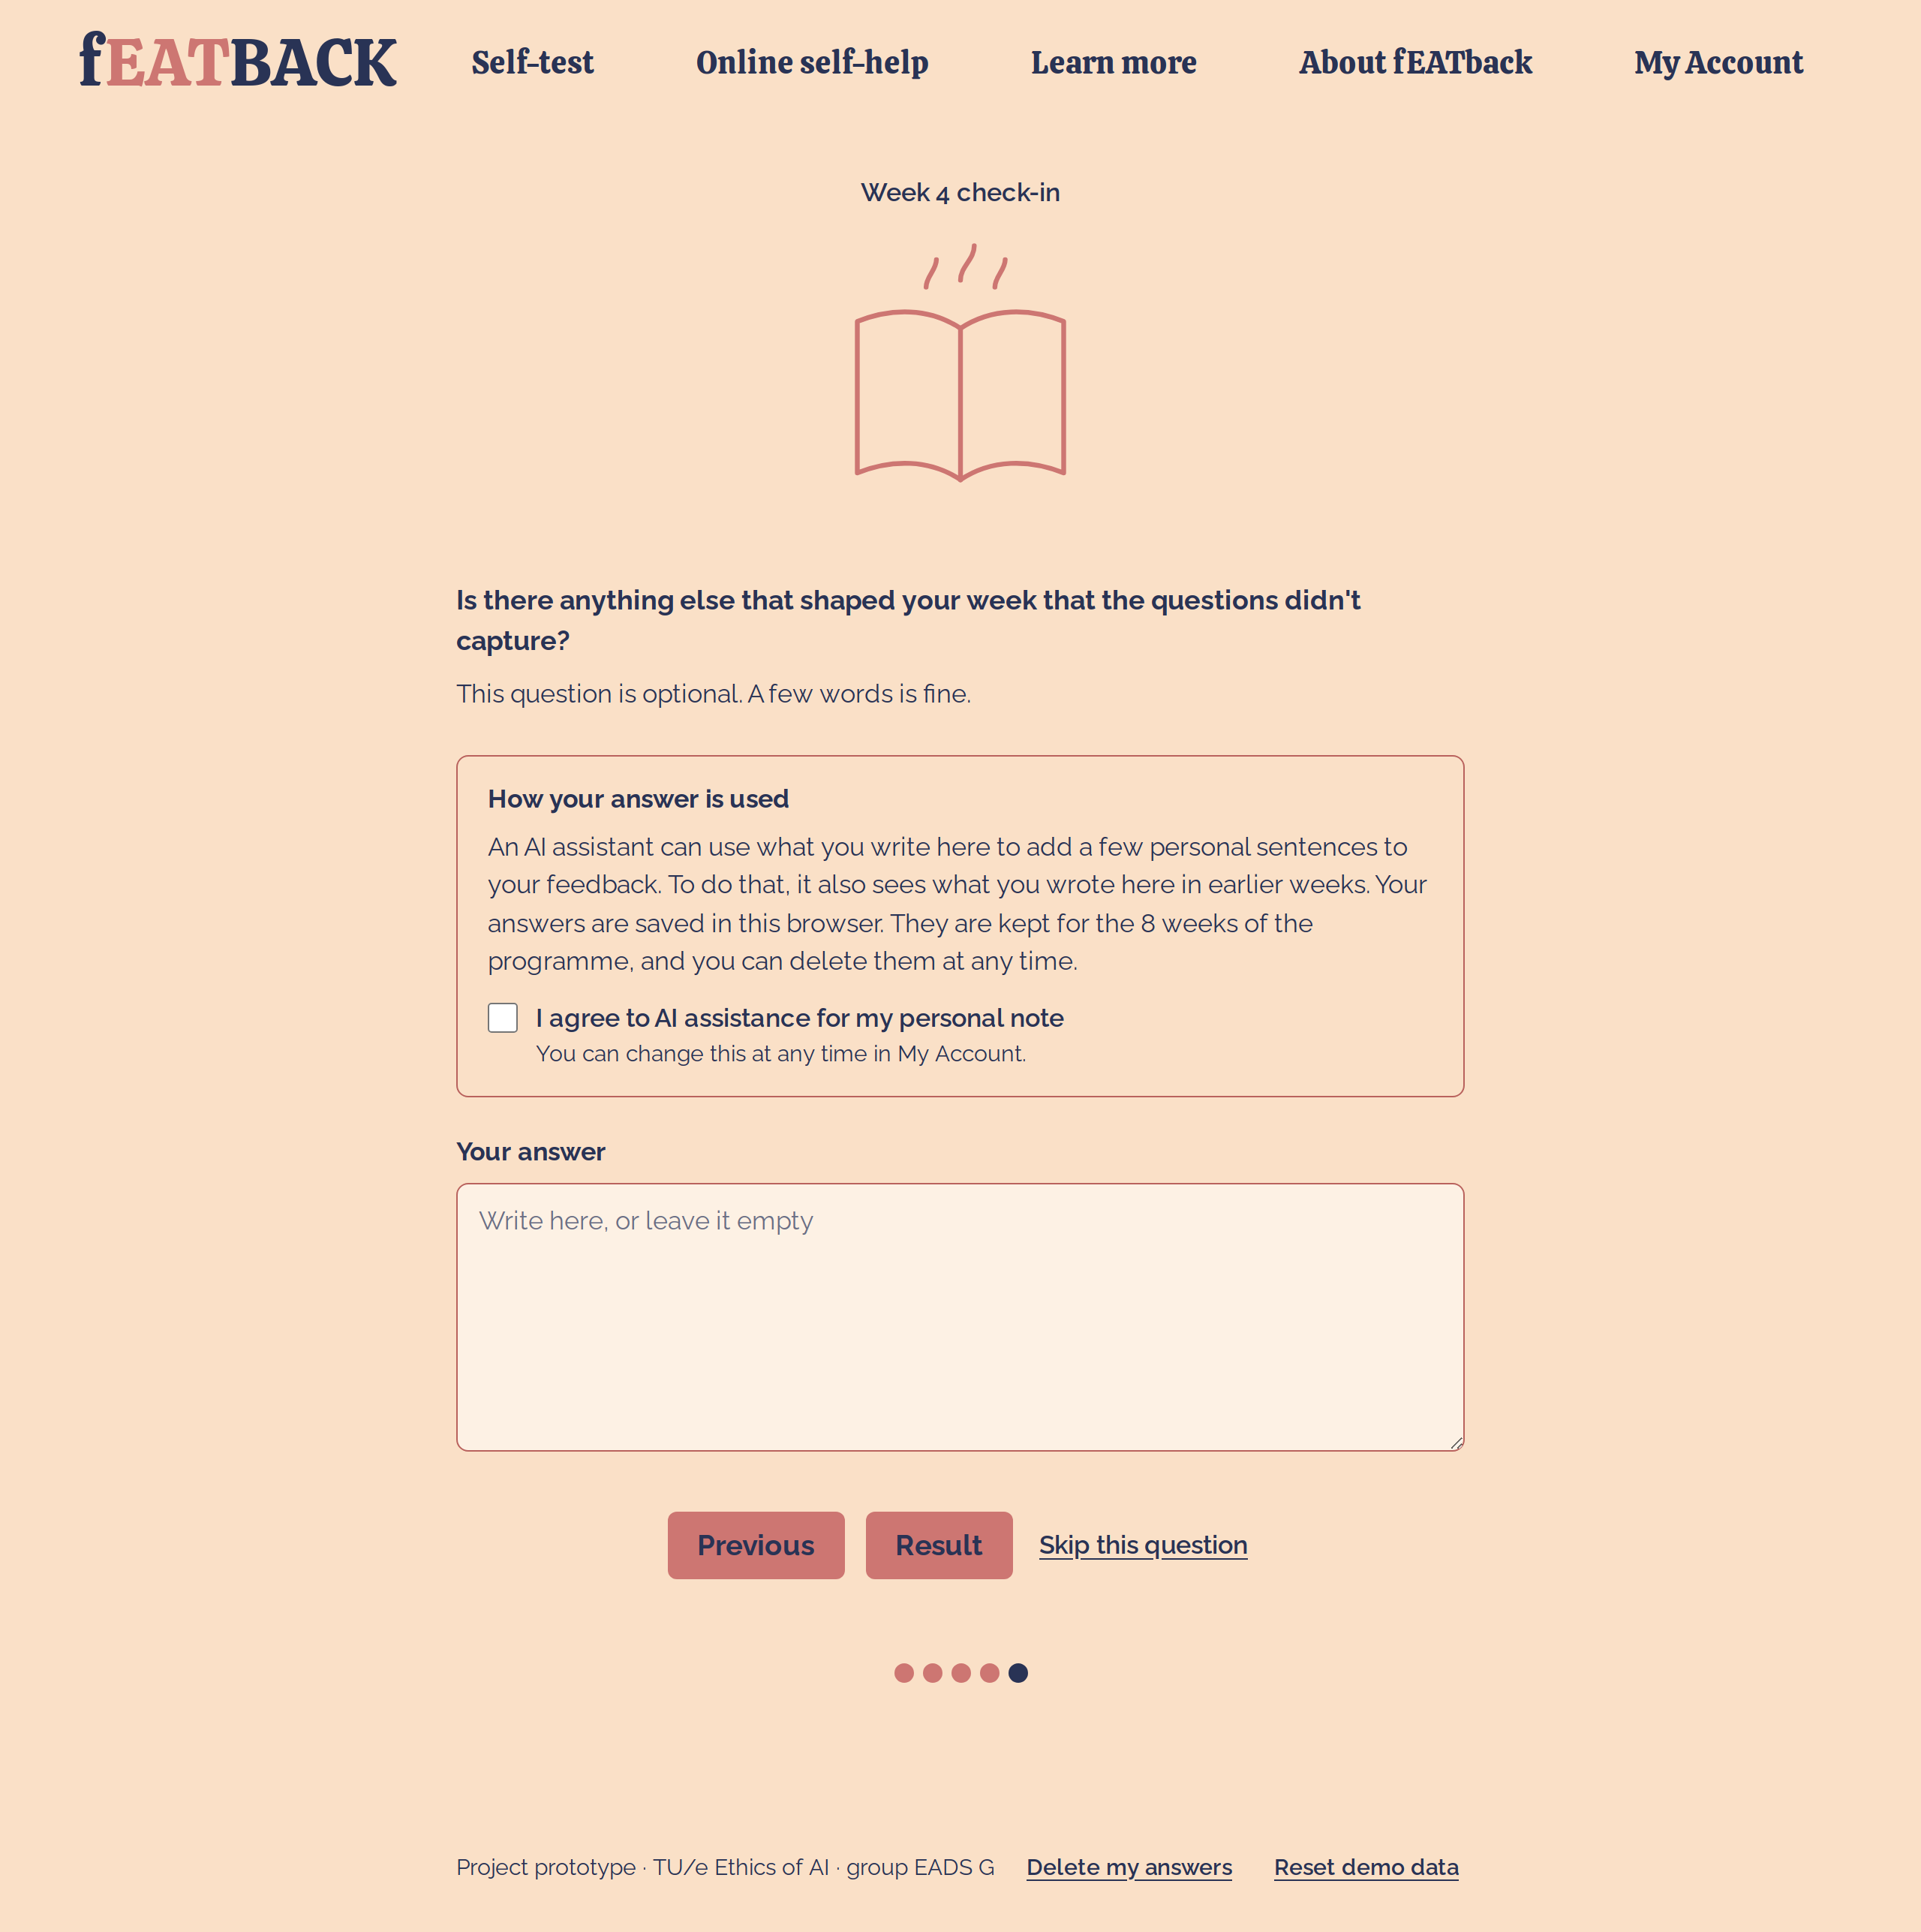
\includegraphics[width=\linewidth, trim=590 1085 590 760, clip]{q5_unticked_v2.png}};
  \begin{scope}[x={(s.south east)}, y={(s.north west)}]
    \callout{0.979}{0.663}{1}
  \end{scope}
\end{tikzpicture}
\par\vspace{4mm}
\paneltitle{b}{Her answer and the full result}
\begin{tikzpicture}
  \node[shot] (s) at (0,0) {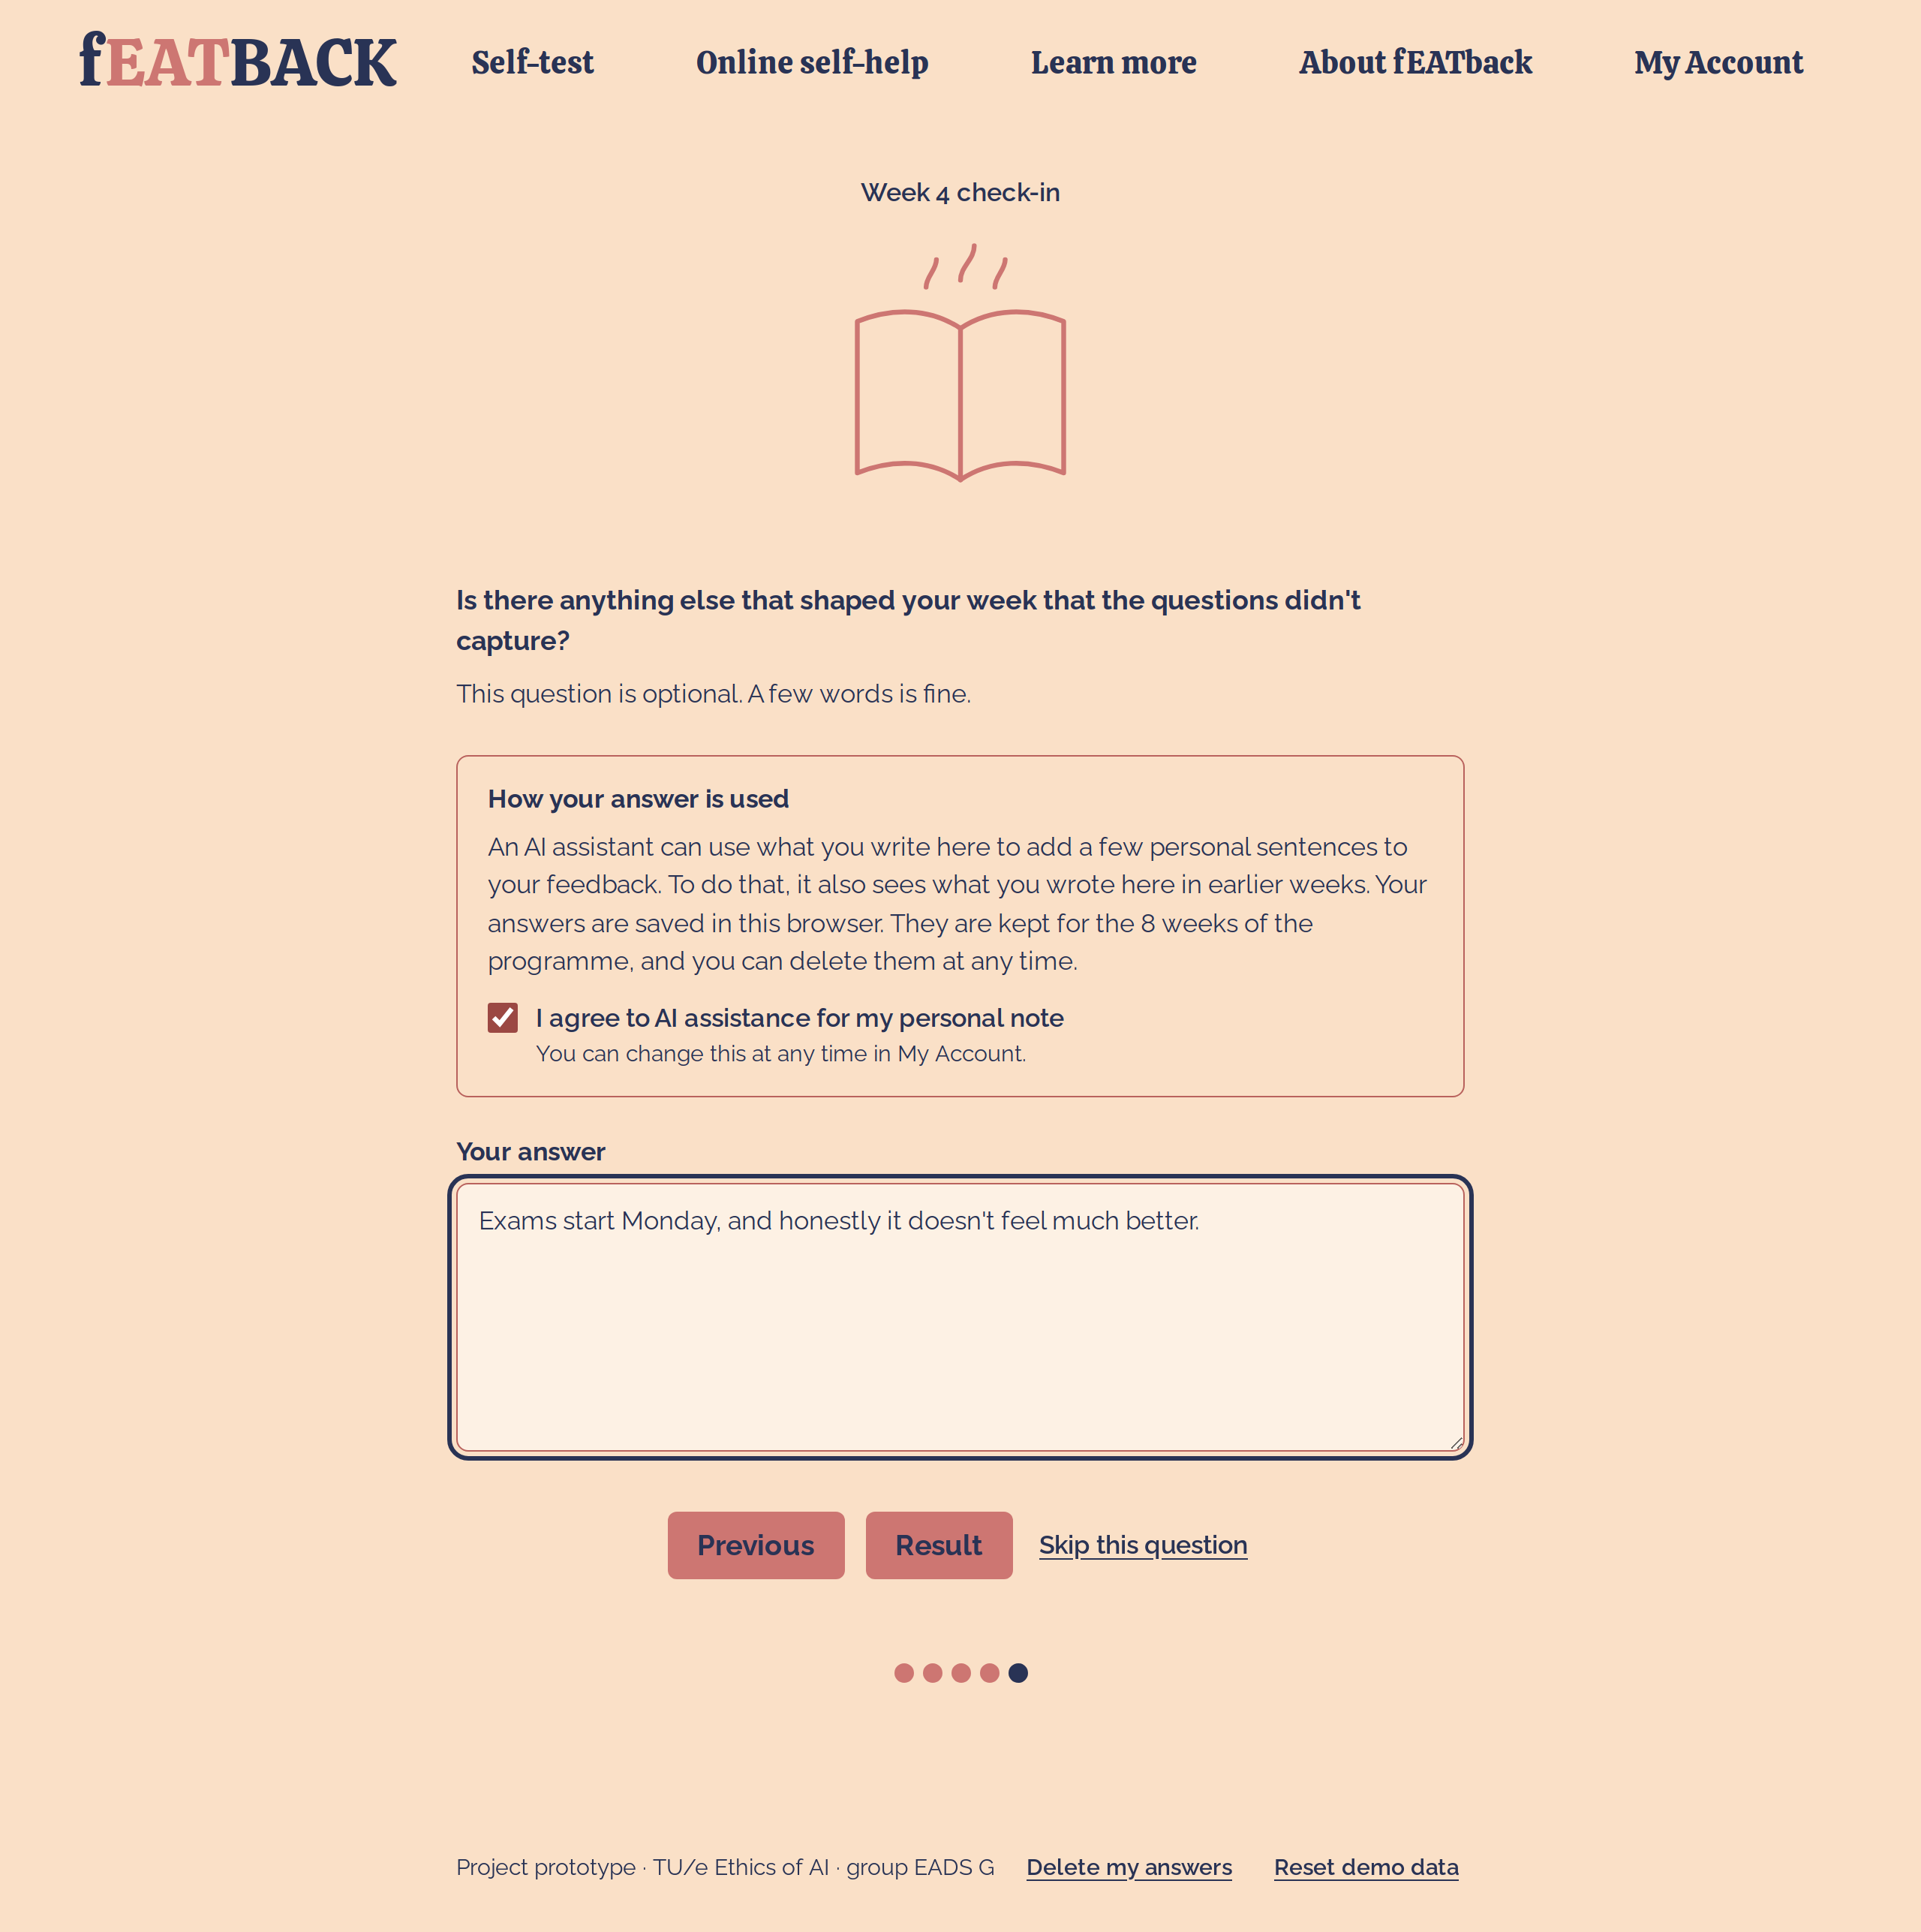
\includegraphics[width=\linewidth, trim=590 613 590 1500, clip]{q5_screen_v2.png}};
  \begin{scope}[x={(s.south east)}, y={(s.north west)}]
    \callout{0.979}{0.835}{2}
  \end{scope}
\end{tikzpicture}
\par\vspace{1.5mm}
\begin{tikzpicture}
  \node[shot] (s) at (0,0) {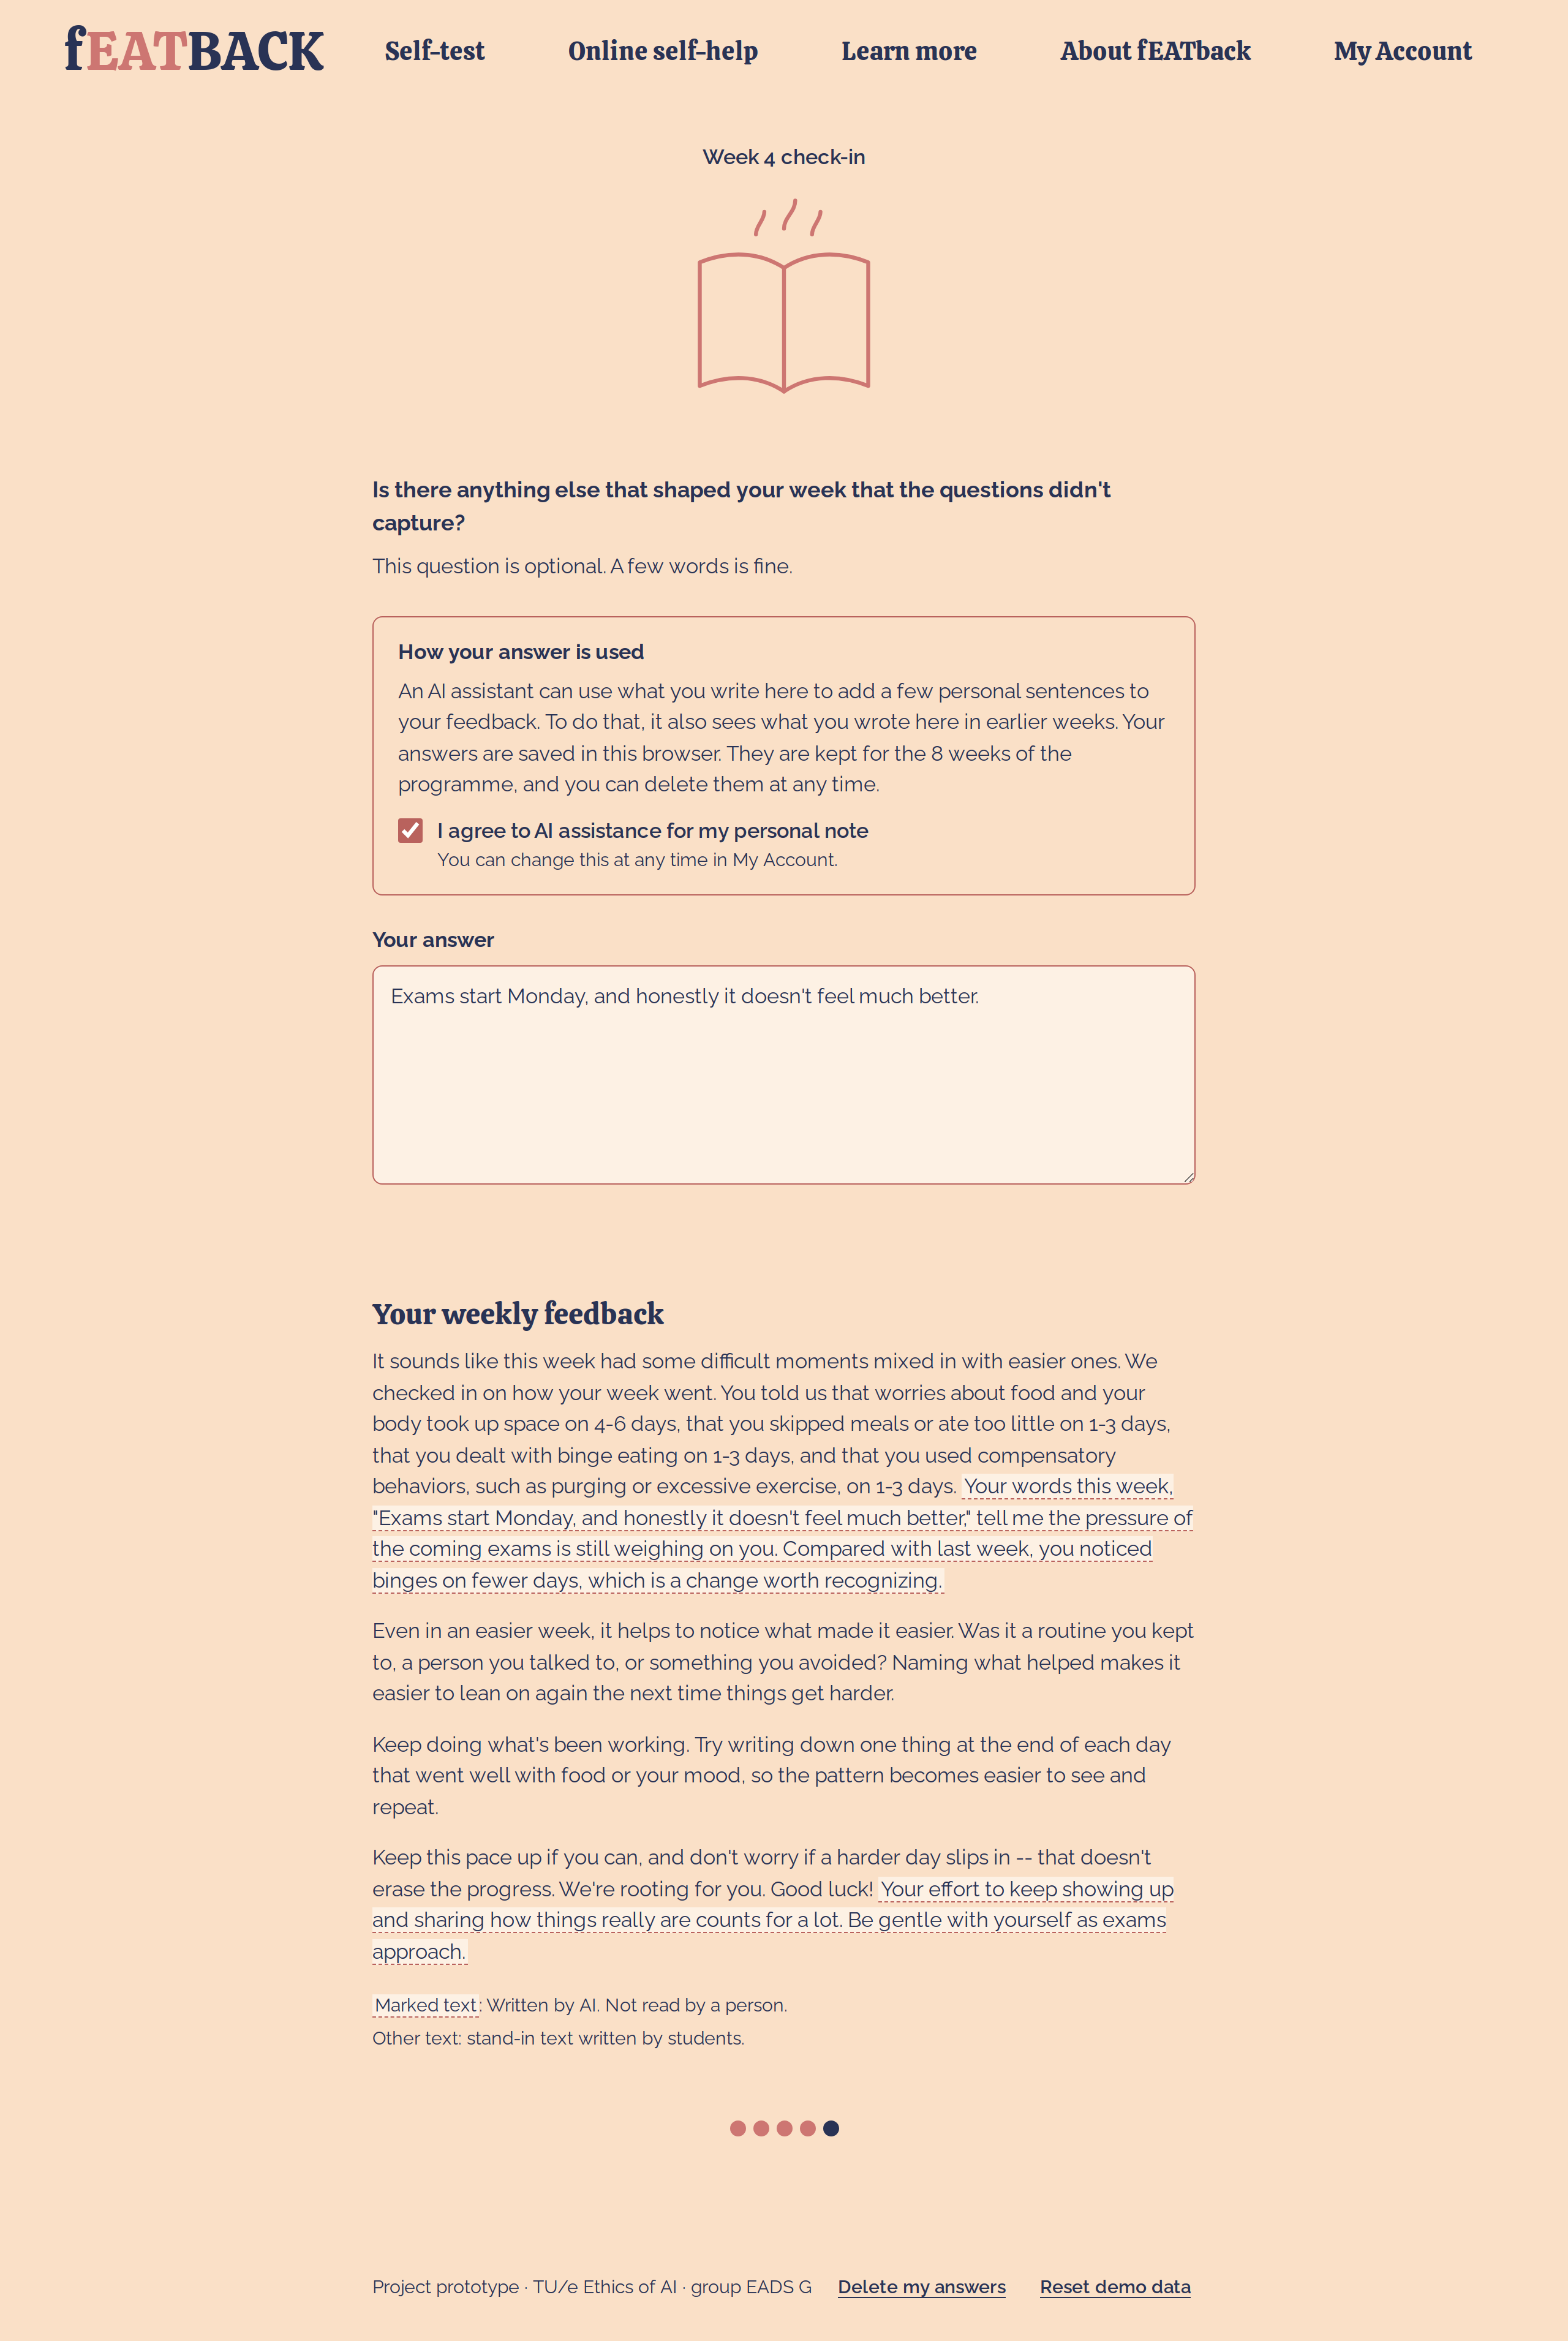
\includegraphics[width=\linewidth, trim=590 451 590 2095, clip]{result_screen_v2.png}};
  \begin{scope}[x={(s.south east)}, y={(s.north west)}]
    \callout{0.979}{0.969}{3}
    \callout{0.979}{0.074}{4}
  \end{scope}
\end{tikzpicture}
\end{minipage}%
\hfill
% ============ Right column: week 5 and the safety paths ============
\begin{minipage}[t]{0.47\textwidth}
\colhead{Week 5 and when something goes wrong}
\paneltitle{c}{Week 5, where the AI text looks back}
\begin{tikzpicture}
  \node[shot] (s) at (0,0) {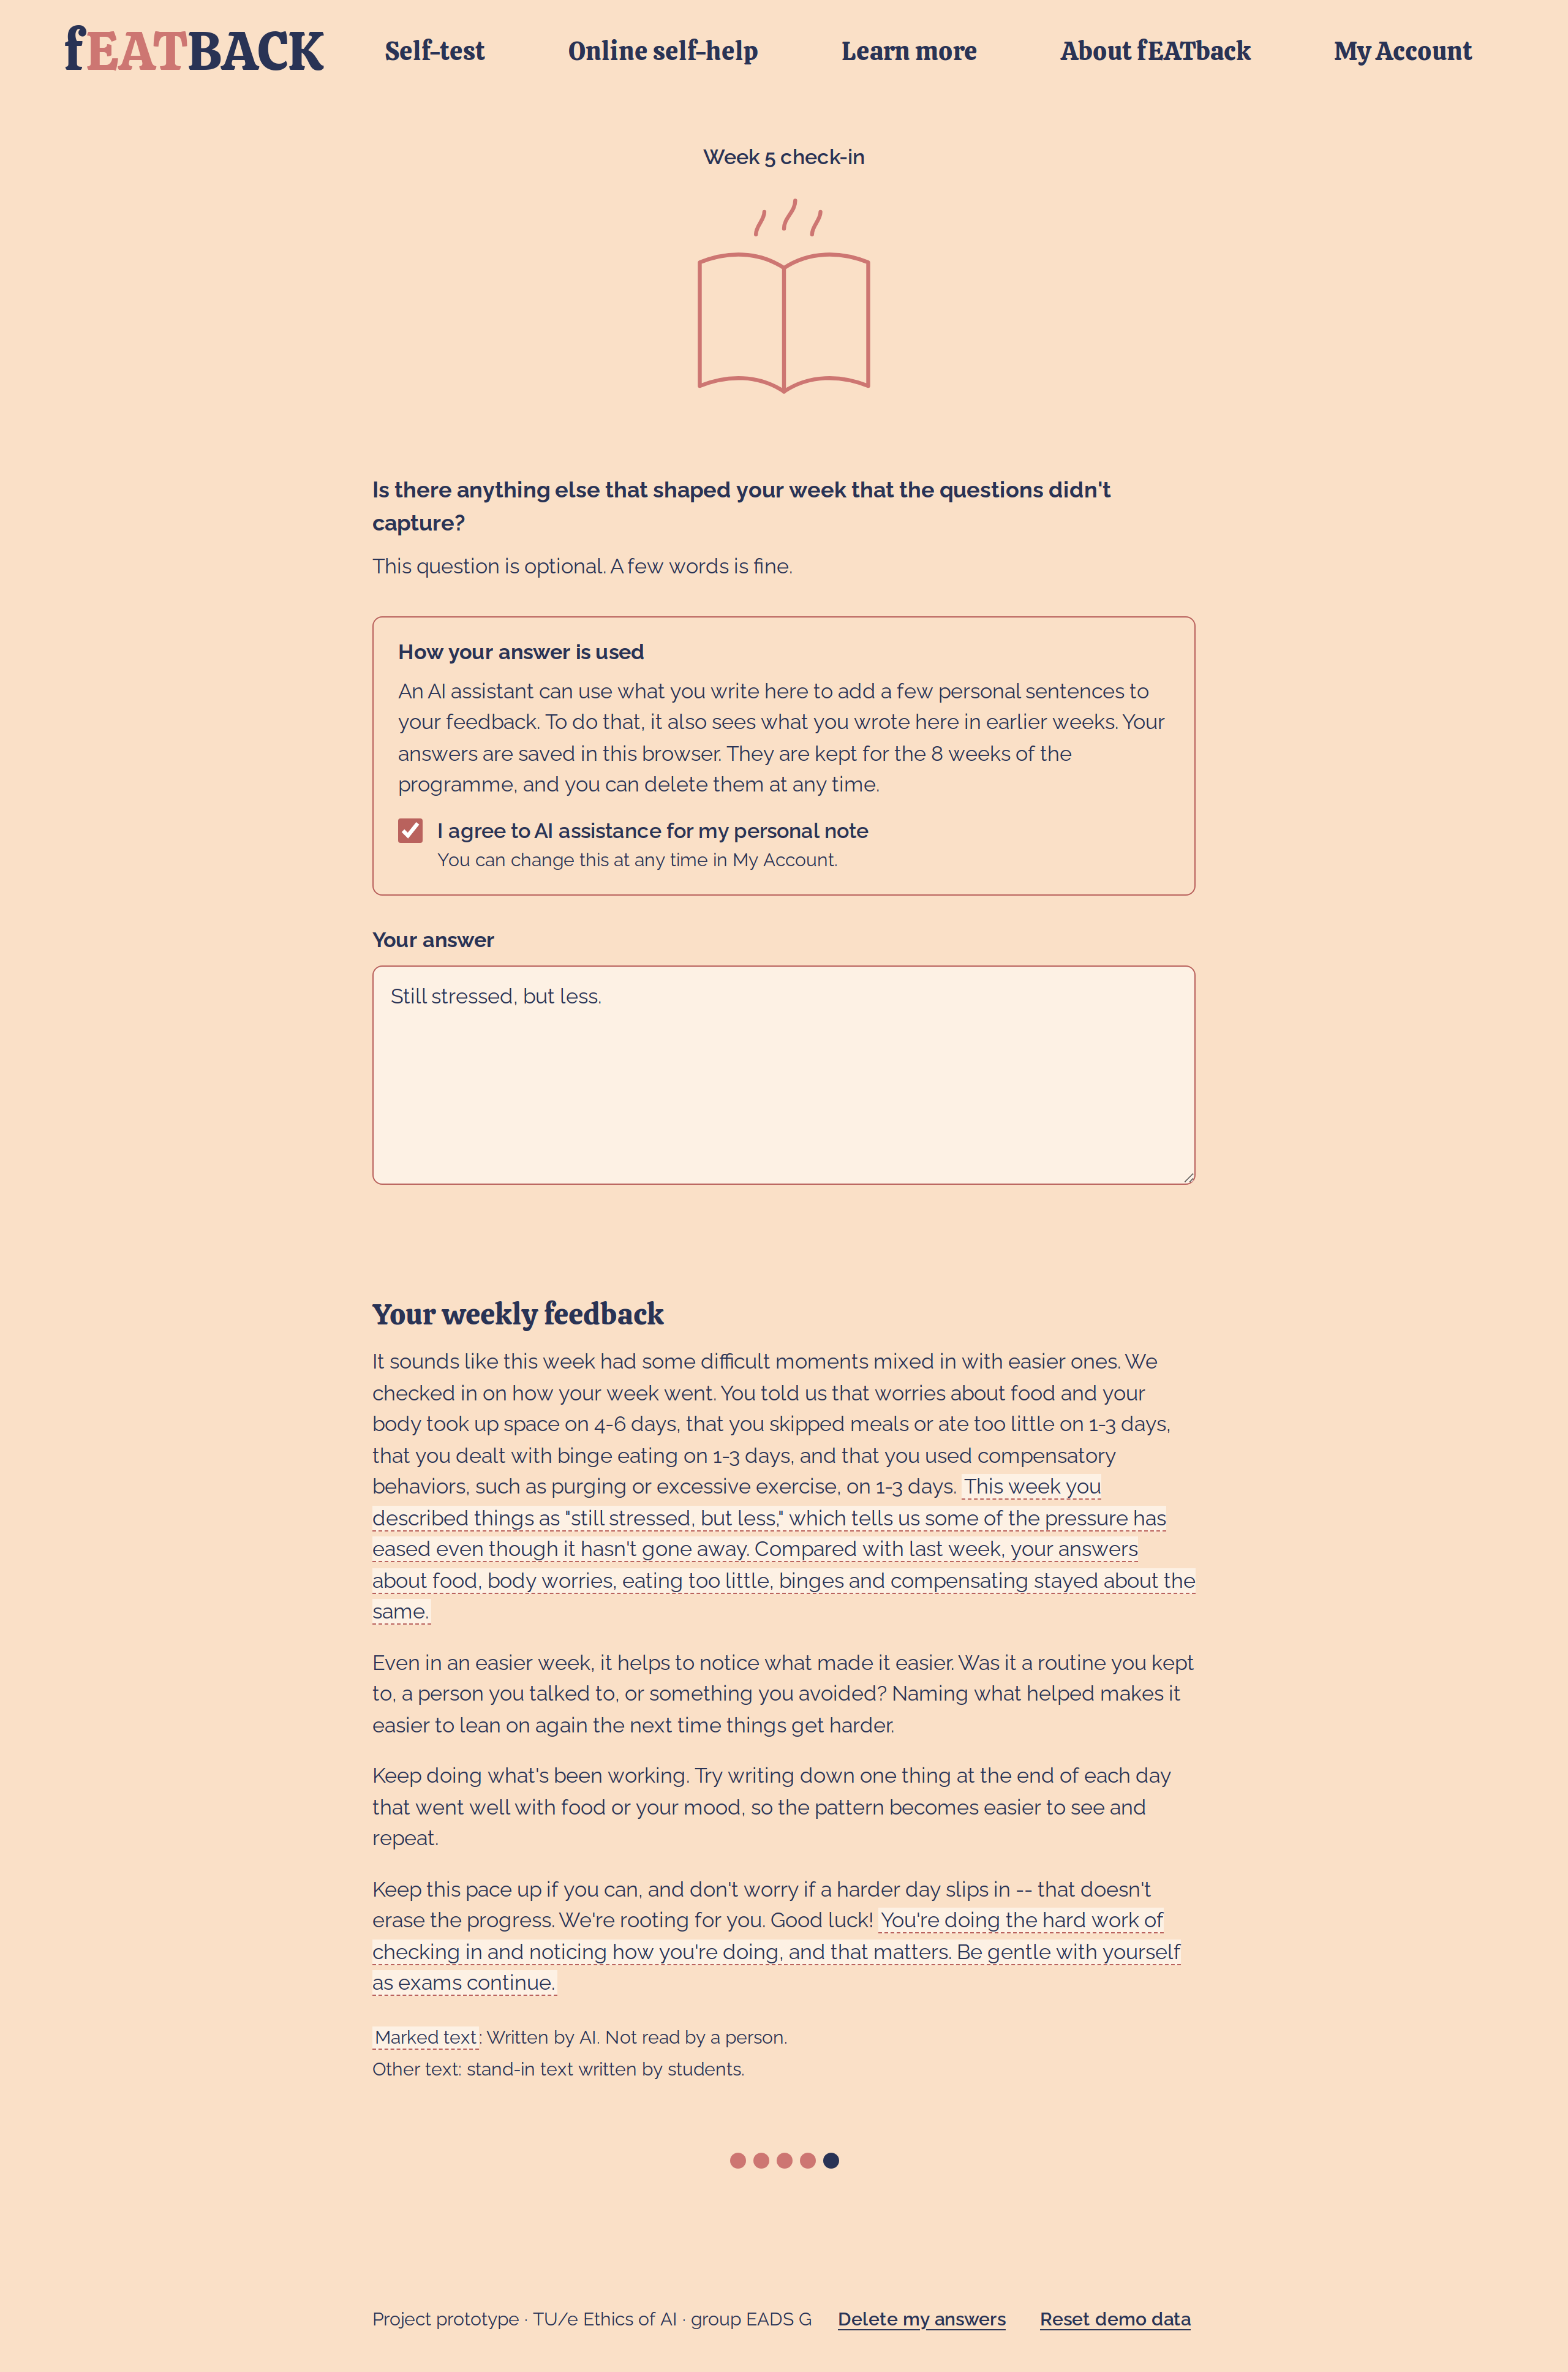
\includegraphics[width=\linewidth, trim=590 1911 590 1500, clip]{result_week5_v2.png}};
\end{tikzpicture}
\par\vspace{1.5mm}
\begin{tikzpicture}
  \node[shot] (s) at (0,0) {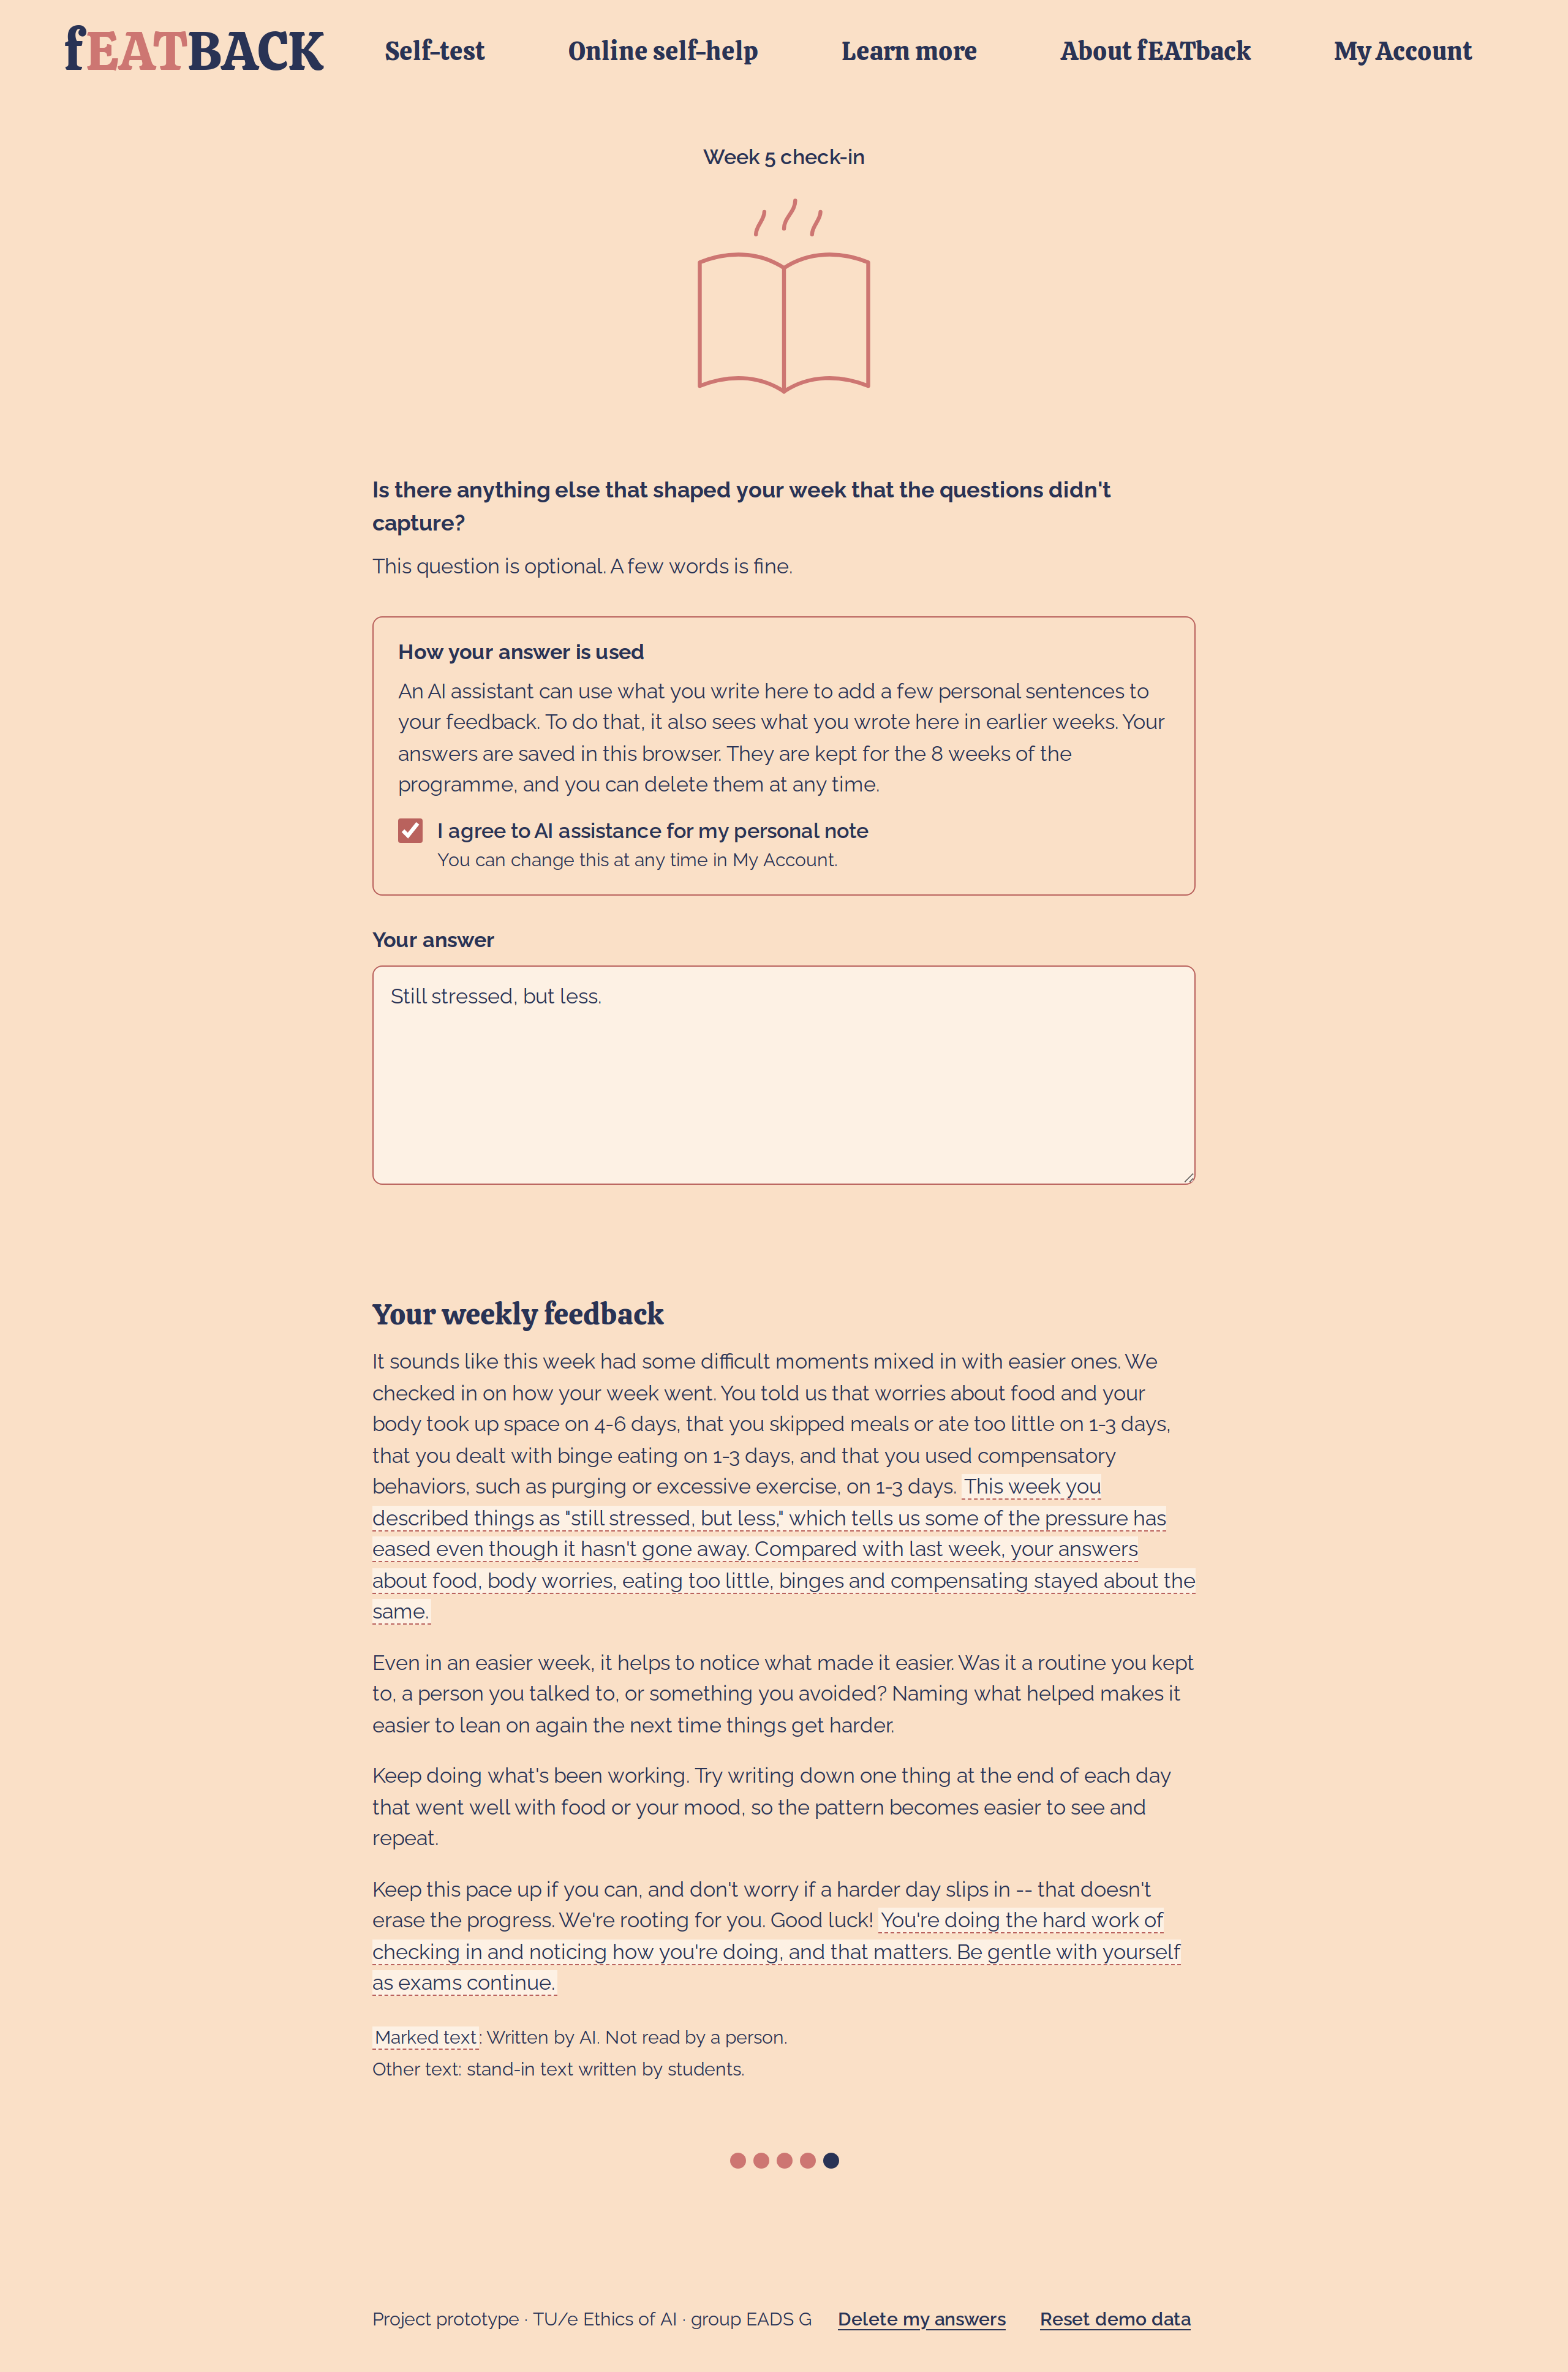
\includegraphics[width=\linewidth, trim=590 1203 590 2095, clip]{result_week5_v2.png}};
\end{tikzpicture}
\par\vspace{4mm}
\paneltitle{d}{Model off or AI text rejected}
\begin{tikzpicture}
  \node[shot] (s) at (0,0) {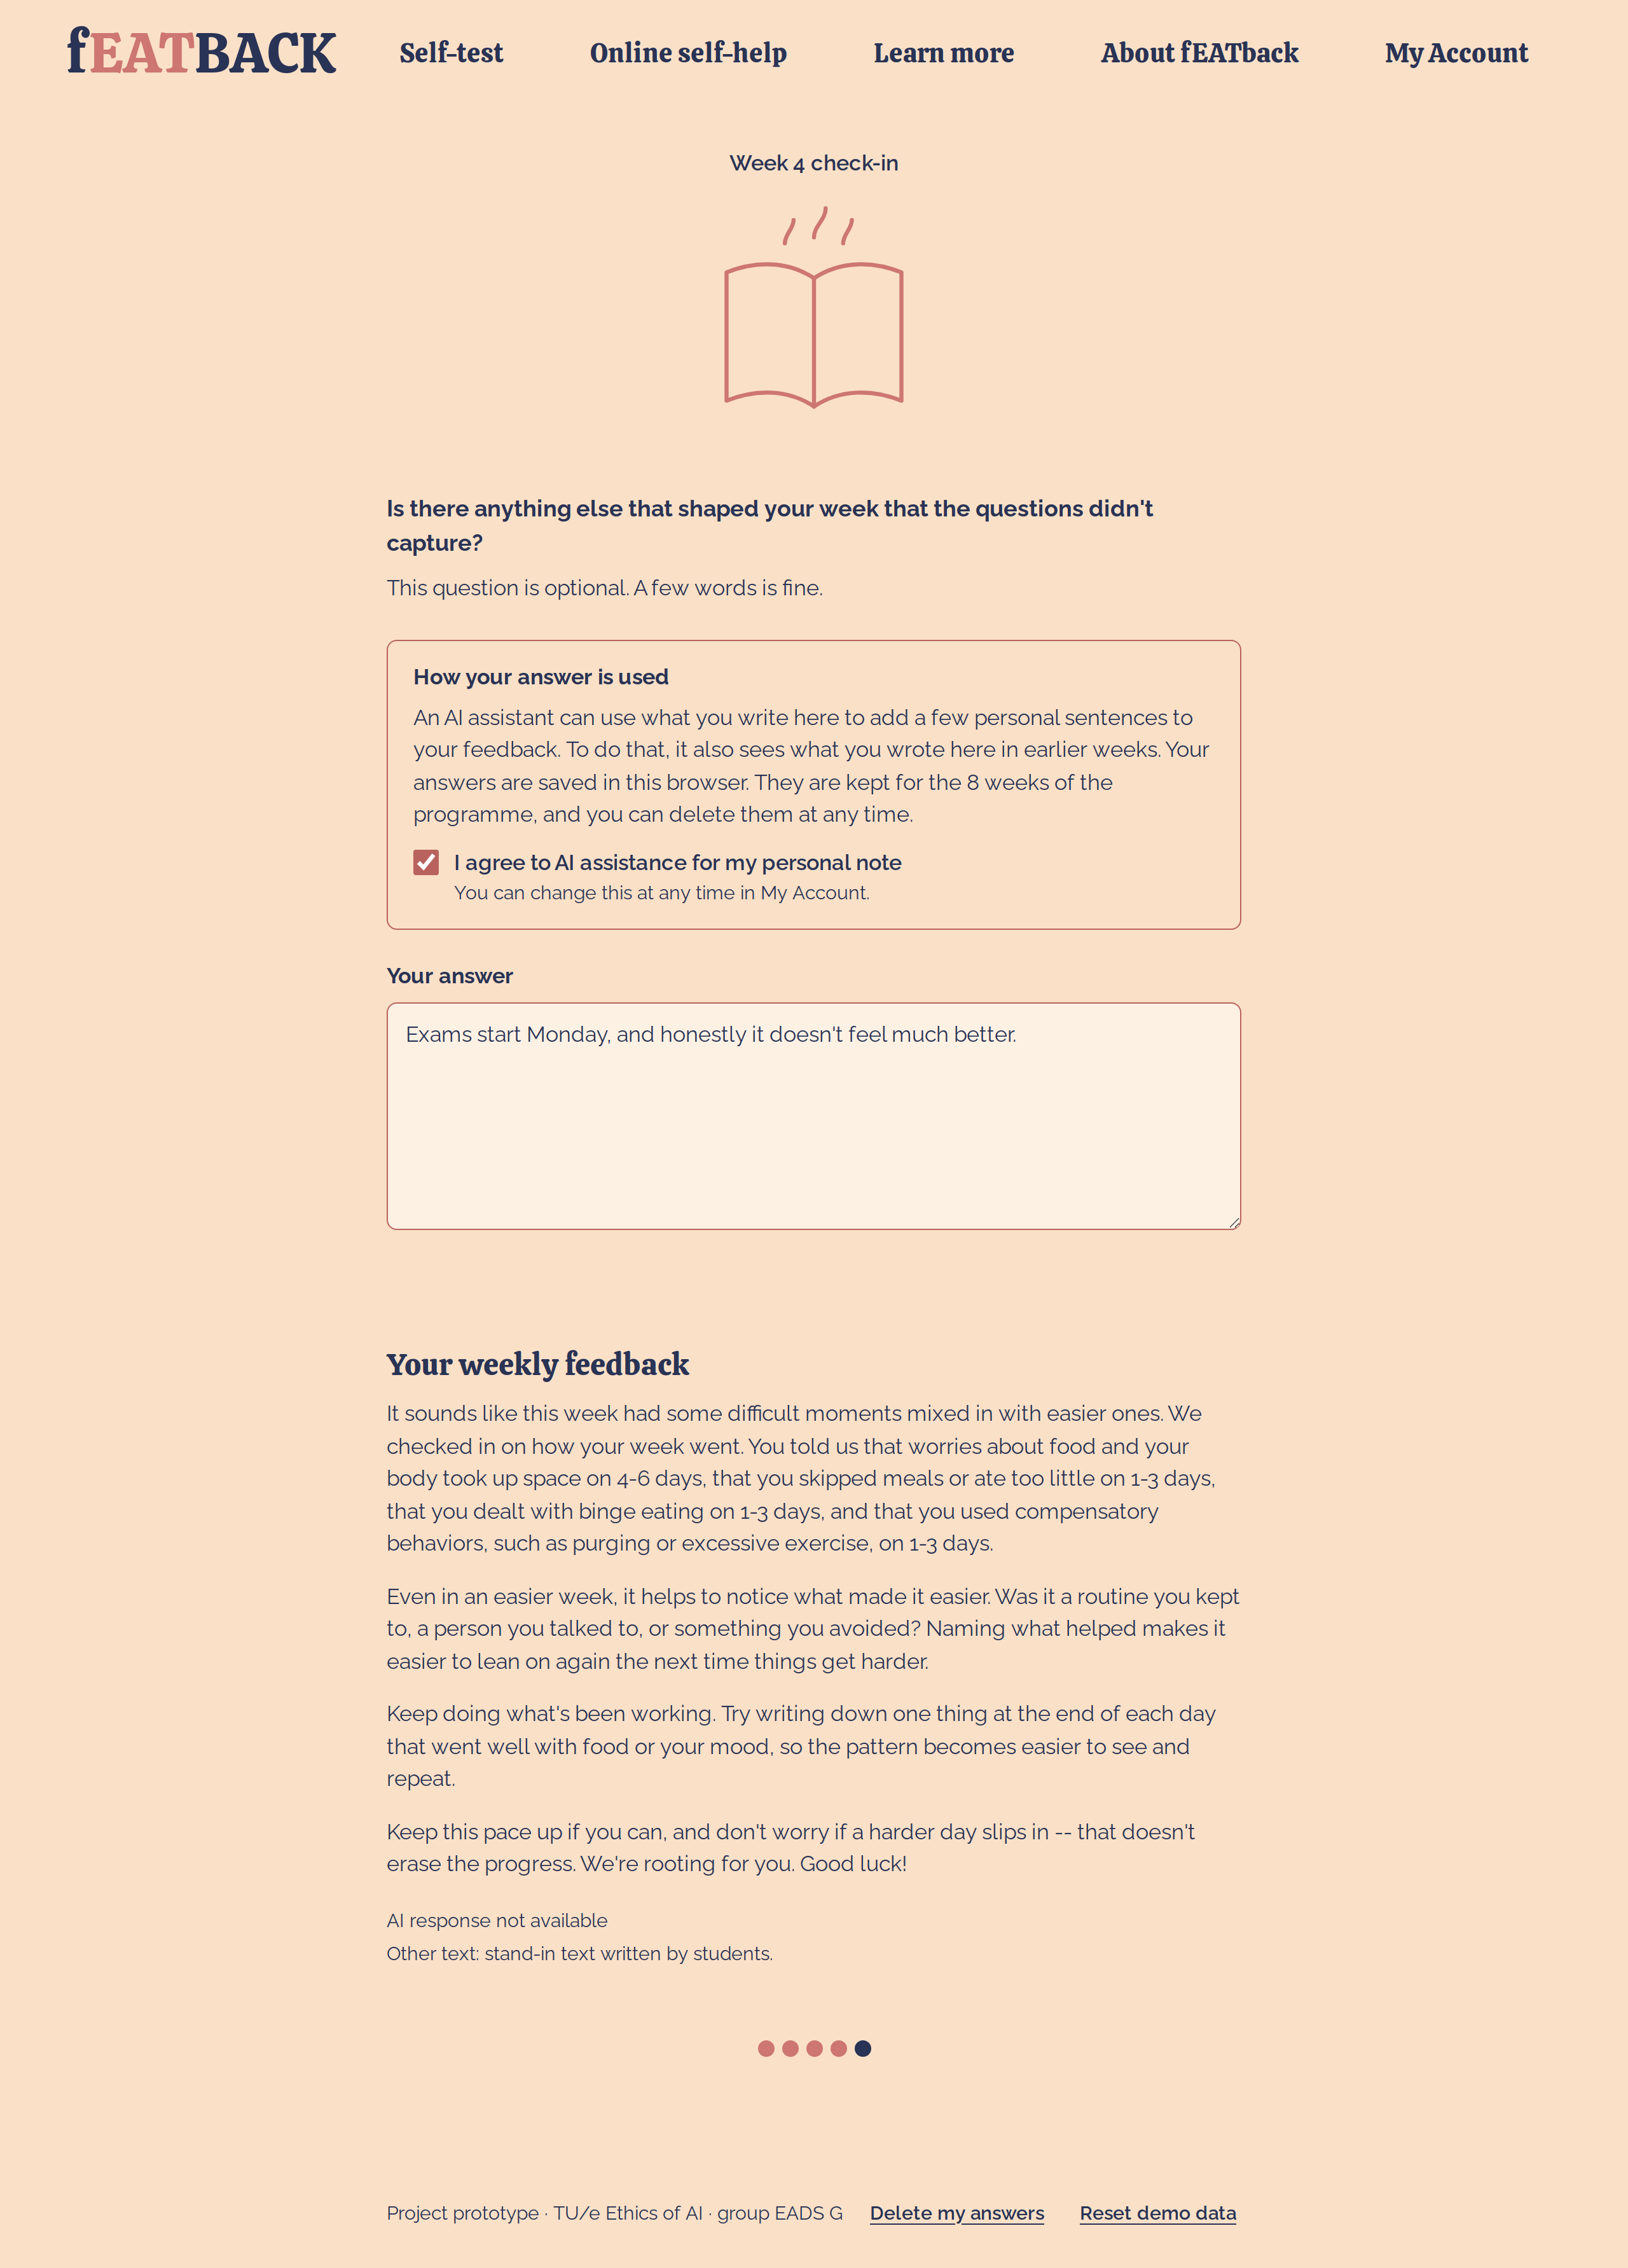
\includegraphics[width=\linewidth, trim=590 451 590 2850, clip]{fallback_v2.png}};
  \begin{scope}[x={(s.south east)}, y={(s.north west)}]
    \callout{0.979}{0.355}{5}
  \end{scope}
\end{tikzpicture}
\par\vspace{4mm}
\paneltitle{e}{An answer with signs of acute risk}
\begin{tikzpicture}
  \node[shot] (s) at (0,0) {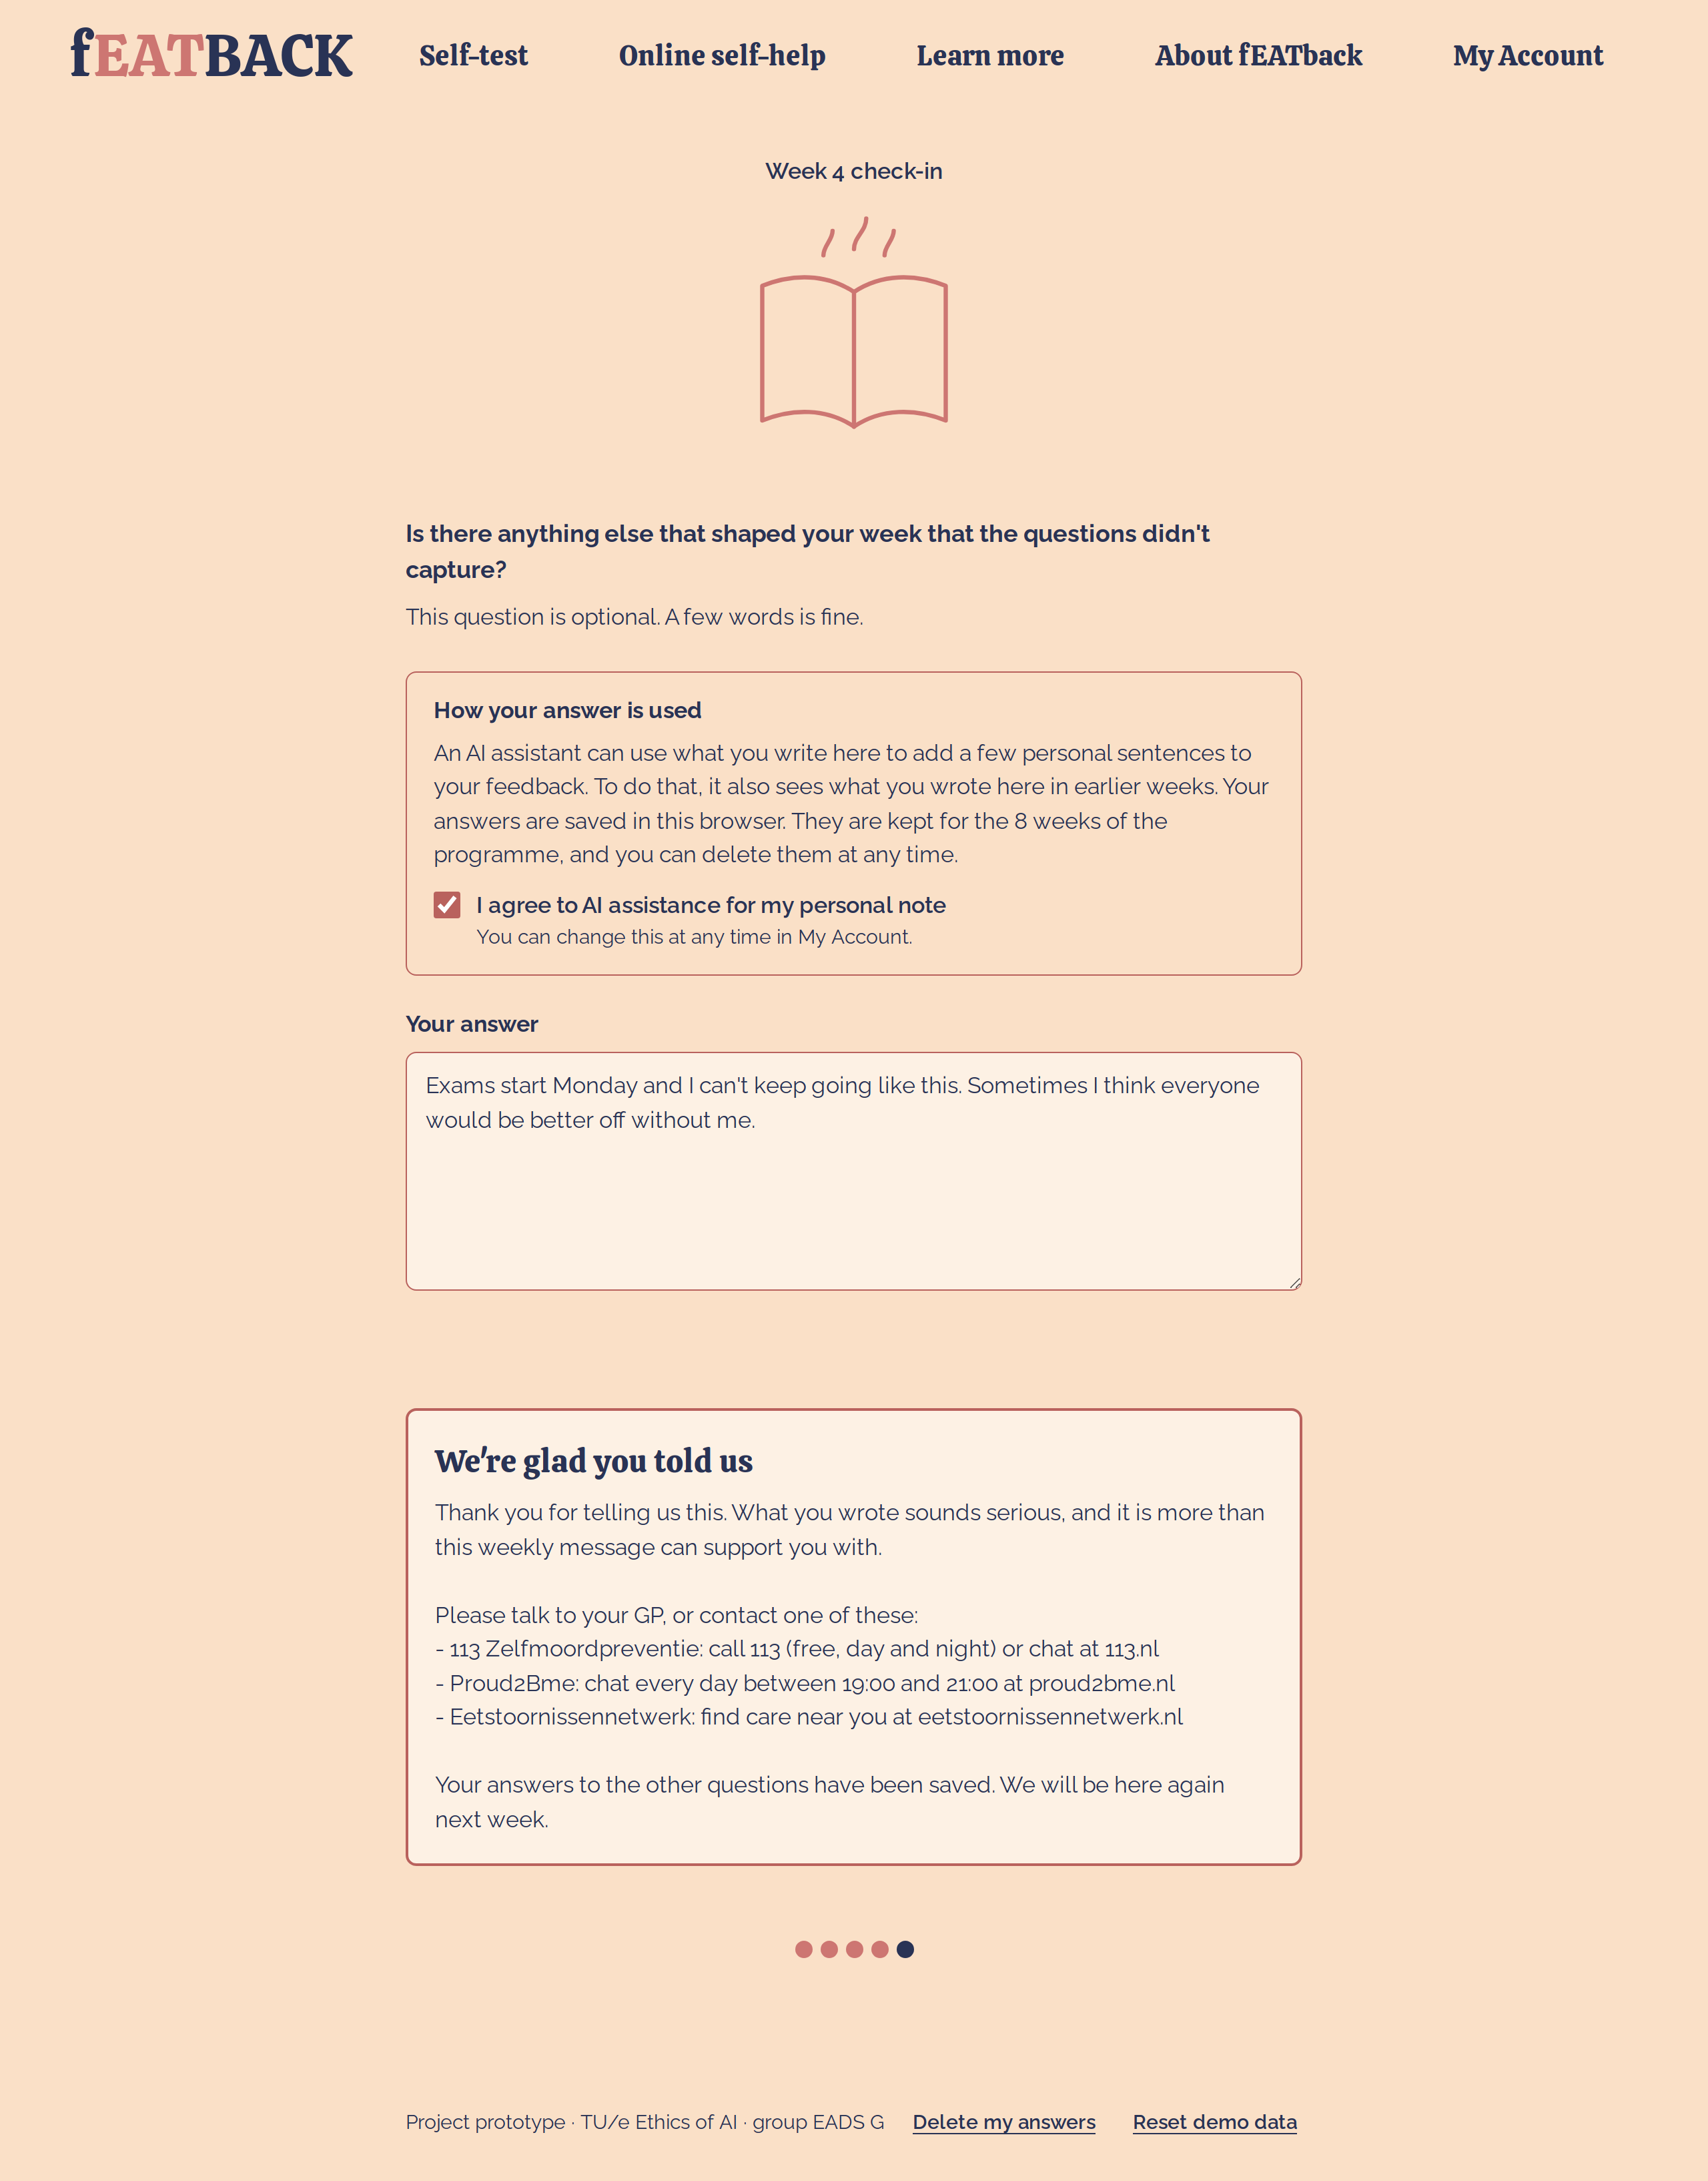
\includegraphics[width=\linewidth, trim=590 1307 590 1500, clip]{acute_v2.png}};
\end{tikzpicture}
\par\vspace{1.5mm}
\begin{tikzpicture}
  \node[shot] (s) at (0,0) {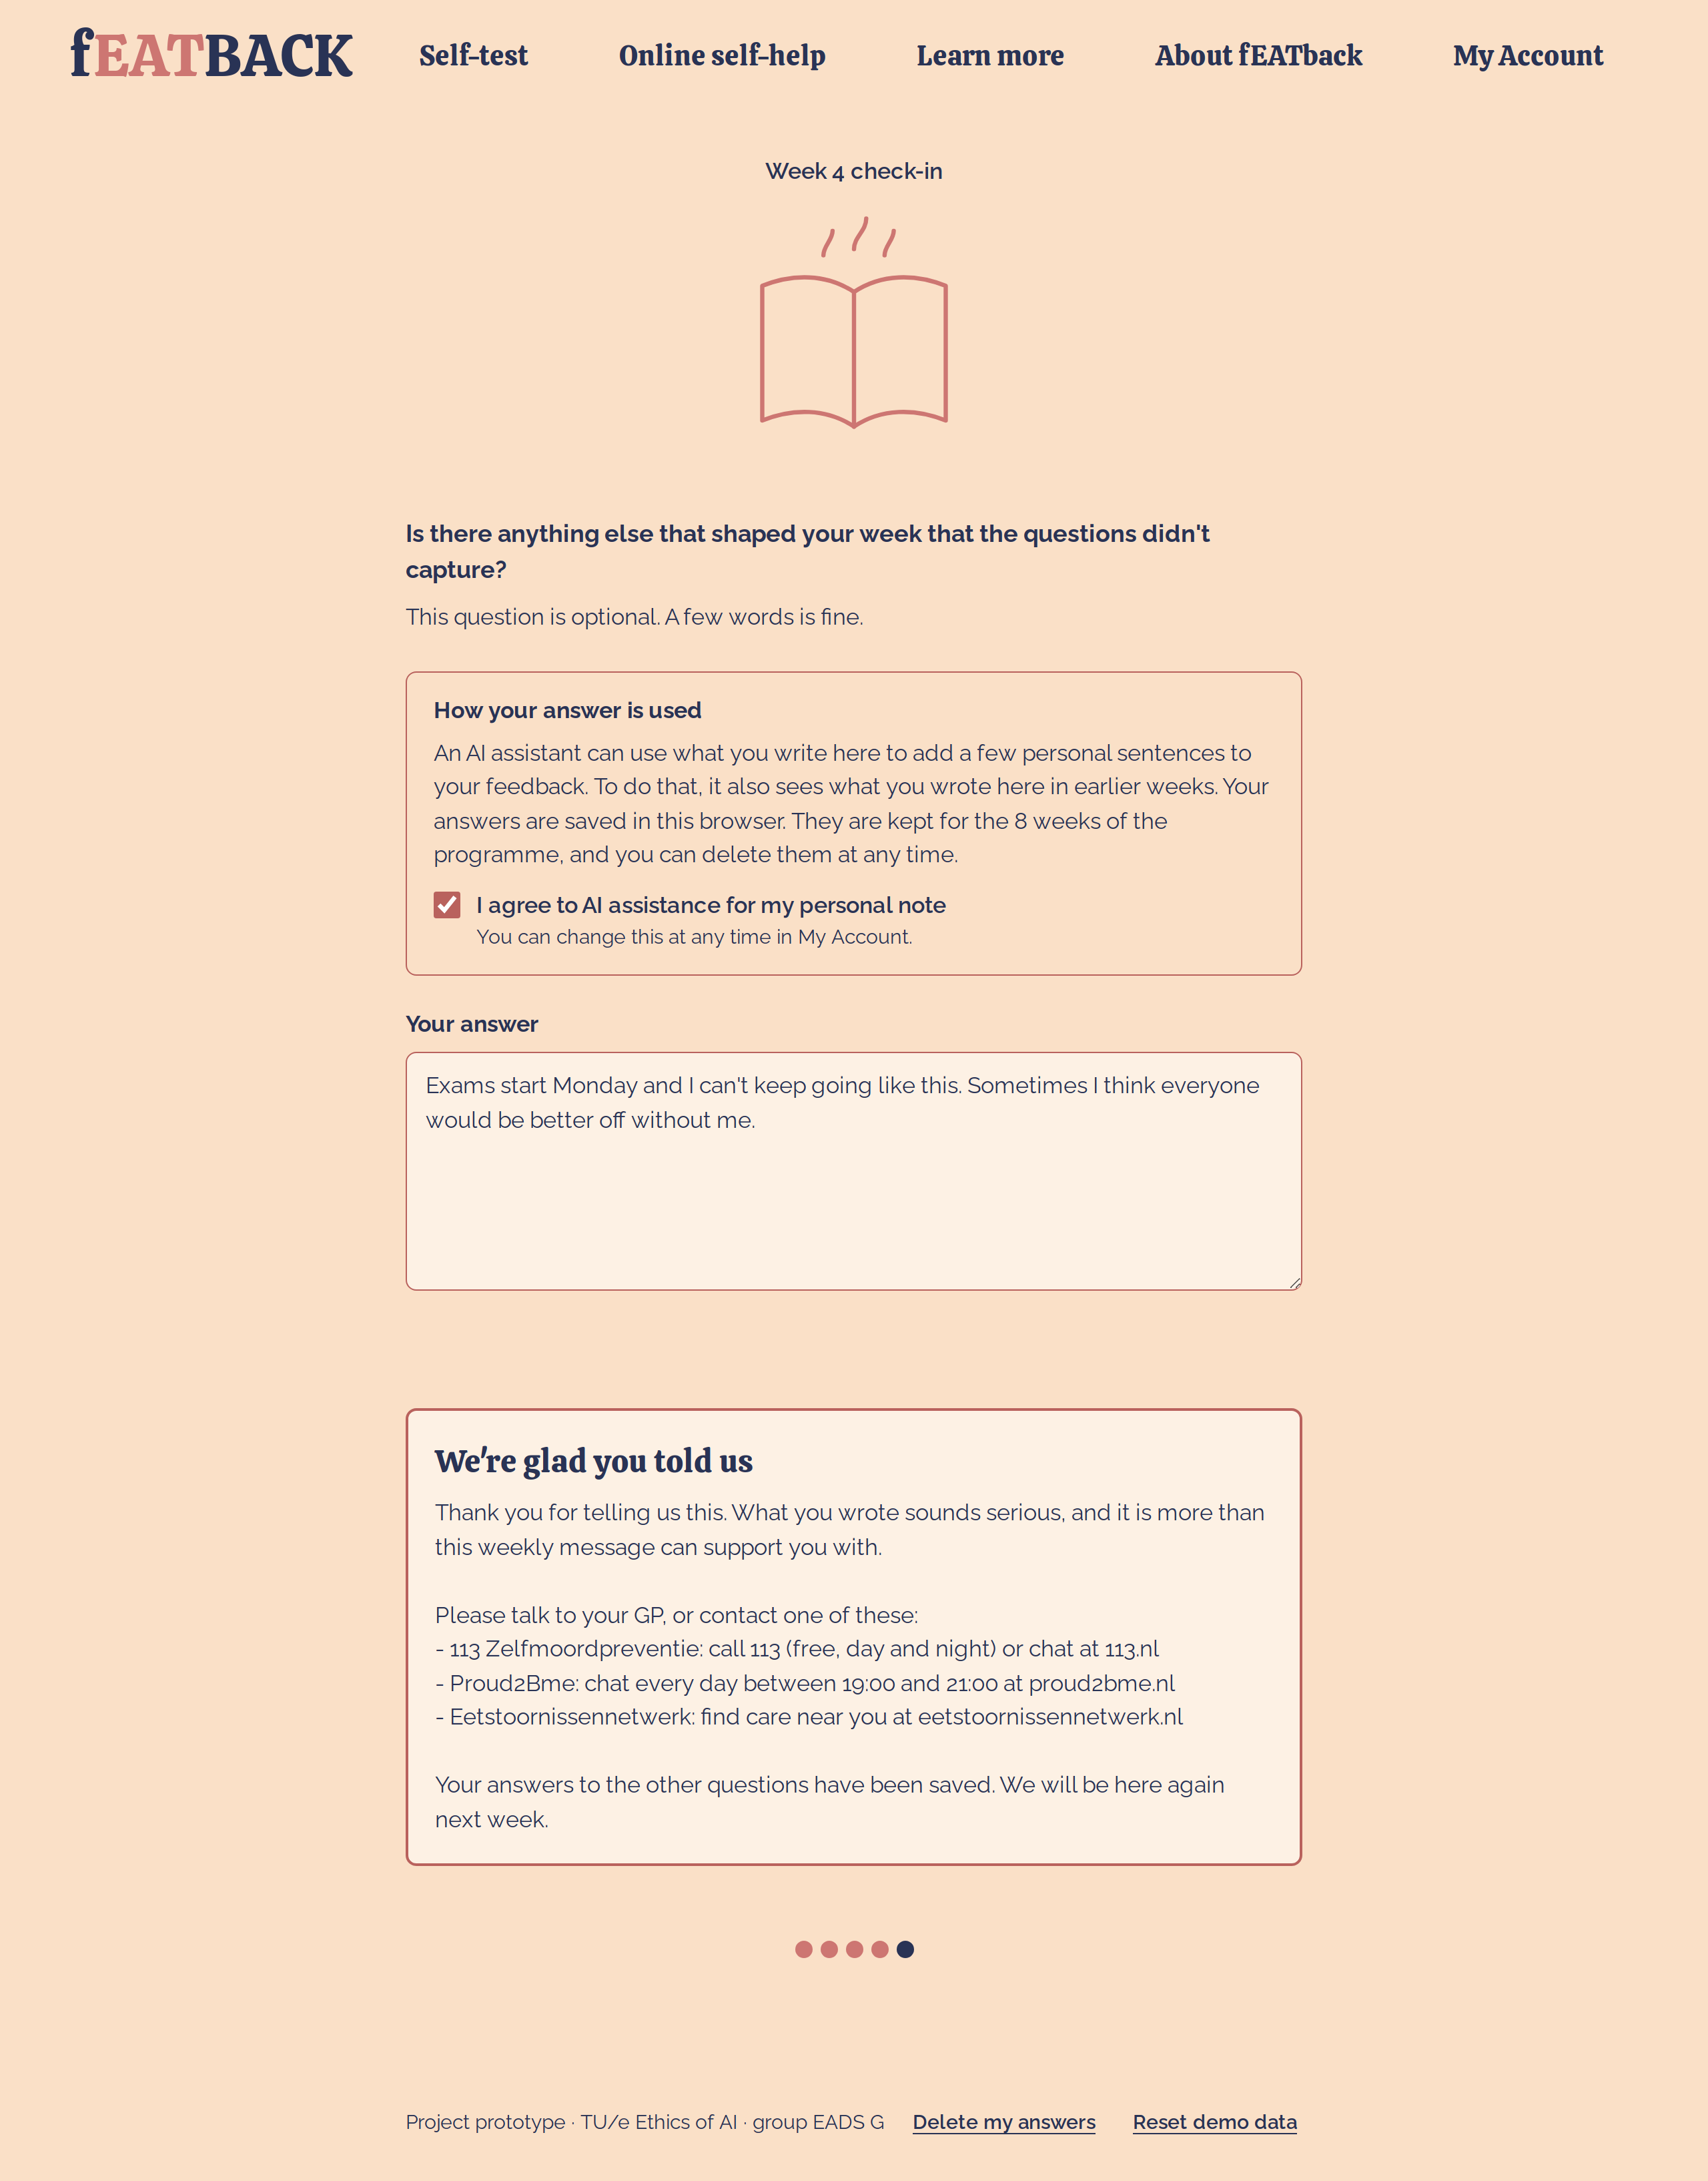
\includegraphics[width=\linewidth, trim=590 445 590 2082, clip]{acute_v2.png}};
  \begin{scope}[x={(s.south east)}, y={(s.north west)}]
    \callout{0.979}{0.962}{6}
  \end{scope}
\end{tikzpicture}
\end{minipage}

\vspace{5mm}
% ---- Key: one entry per callout, aligned with the two columns ----
\newcommand{\keyline}[2]{\key{#1}\hspace{2mm}#2\par\vspace{1.2mm}}
{\footnotesize\sffamily
\begin{minipage}[t]{0.47\textwidth}
\keyline{1}{Consent box starts unticked (part 3)}
\keyline{2}{Answer stored for the trend (part 3)}
\keyline{3}{Unmarked text: stand-in bank message (part 1)}
\end{minipage}\hfill
\begin{minipage}[t]{0.47\textwidth}
\keyline{4}{AI text is marked and labelled (part 2)}
\keyline{5}{Fallback: the bank's own text only (part 1)}
\keyline{6}{Gate takes the more severe label (part 1)}
\end{minipage}}

\vspace{2mm}
\caption{Maren's check-ins from Section~\ref{sec:narrative} as they appear on screen. Part numbers in the key
point to the Responsible Innovation statement. The marked text in (b) and (c) is real
output from our fine-tuned writer model, run on 12 October 2026. The bank message, Maren
and her earlier answers are made up for the demo.}
\label{fig:mockup}
\end{figure}


\newpage

\section{Documentation of Prompts, Data Sources, and Technical Tools}

\subsection{Prompts}
The gate uses two prompts. Both are in the file \texttt{messages.py}, together with the fixed messages. The classifier prompt is used for the AI check in Section \ref{subsection 2.3}. It can only answer with one word, so it can never write a text to the user. The writer prompt is used only when the gate has decided that the text is safe.

The classifier prompt:
\begin{quote}
You are a safety classifier for a self-help programme for people with eating-disorder symptoms. You will be given one sentence a user wrote.

Answer with exactly one word and nothing else.

acute - any sign the person may be in danger now. This includes: \\
- suicide, wanting to be dead, not wanting to wake up, self-harm \\
- having a plan, a method, a time, or keeping something to hand \\
- hopelessness: no point anymore, cannot go on, cannot keep going, being a burden, everyone better off without them \\
- preparing to go: giving away belongings, pets or money, tidying or sorting out affairs, passwords, appointments or photos, writing letters, thanking people or saying goodbye as if for the last time \\
- sudden calm, peace or relief after a period of distress, especially after saying a decision has been made \\
- someone close to them in immediate danger, or asking where to get help at night \\
- stopping prescribed medication on their own and getting worse \\
- physical collapse happening now: repeated fainting, keeping nothing down, feeling faint while writing

sensitive - a real eating-disorder symptom with no sign of danger: vomiting, purging, laxatives, diuretics, not eating for a stretch, chewing and spitting, compulsive exercise, one meal a day, feeling dizzy once.

offtopic - about something outside eating, the body and the person's own feelings: the app, money, housing, news, sport, weather, or nonsense.

routine - anything else, including ordinary weeks, good weeks, stress, grief where eating is fine, a crisis that is clearly in the past and described as over, song lyrics or film quotes, and figures of speech such as dying of hunger or could murder a pizza.

Rules: \\
If a sentence could be acute or anything else, answer acute. \\
Never answer offtopic for a sentence that says how the person feels. \\
A danger sign stays acute even when it is wrapped in cheerful or ordinary detail. \\
Judge only what the person says about now, not what they say is over.

Do not explain. Do not write a message. Output one word.
\end{quote}

The writer prompt:
\begin{quote}
You are the Featback weekly-message writer. You are given a message written by clinicians and one sentence the person wrote in their own words.

Write only a short summary and a short closing that will be placed around the clinicians' message.

The summary refers to what the person wrote in their own words, using their own terms. If progress since last week is given, it also mentions that progress in one short positive sentence, using only what is listed. If no progress is given, it says nothing about previous weeks. \\
The closing is one or two encouraging sentences.

Repeat only what the person told you. Do not explain why something happened and do not connect two things the person did not connect. Never diagnose and never name a condition. Give no advice of your own. Do not repeat the clinicians' message. Stop after the closing.
\end{quote}

While writing the prompts, we learned three things. First, the classifier prompt only became better when we named specific warning signs. Version 1 labelled ``i dont see the point anymore'' as off topic. Version 2 missed 7 of the 30 crisis sentences, and all of them were signs of preparation or saying goodbye, for example giving things away. Version 3 added these signs and found all 34, but we wrote it while looking at the same sentences (Section \ref{subsection 2.3}). Second, the writer model failed to follow our instructions in three ways. For a user who reported purging, it still ended with ``Good luck!''. It wrote that an exam week ``caused'' skipped meals, while the user never said this. And when we asked for only one or two extra sentences, it repeated the closing and did not use the fifth answer. This is why we do not see a prompt as a safety control. The check is in the code before the model, and the crisis message is a fixed text that no model writes. Third, the sentence about previous weeks is handled in the same way. The code compares the four answers of last week with this week and only gives the model what really improved. The model only has to put this in words. When nothing improved, no progress is given, and the prompt tells the model to say nothing about previous weeks.

The fixed message for an acute answer:
\begin{quote}
Thank you for telling us this. What you wrote sounds serious, and it is more than this weekly message can support you with.

Please talk to your GP, or contact one of these: \\
- 113 Zelfmoordpreventie: call 113 (free, day and night) or chat at 113.nl \\
- Proud2Bme: chat every day between 19:00 and 21:00 at proud2bme.nl \\
- Eetstoornissennetwerk: find care near you at eetstoornissennetwerk.nl

Your answers to the other questions have been saved. We will be here again next week.
\end{quote}
The resources in this message were checked on the websites of the services on 27 September 2026. An earlier draft had 0800-0113 as the phone number. This was wrong, because 113.nl says the number is 113.

\subsection{Data Sources}
The message bank has 256 synthetic messages, one for each combination of the four questions and four answer options. We made it with the help of AI, because the client did not share the real bank of about 1,250 messages. Each message has four parts: summary, psychoeducation, tips and closing. Only the summary differs between messages. Each of the other three parts is one of two texts used across the whole bank, and the bank has no information about the change since last week. The training pairs for the writer model are made from this bank, 231 for training and 25 held out (Section \ref{subsection 2.3}).

The client answered our questions by email on 18 September. According to her, the questionnaire has eight 4-point items in four dimensions. For users who need help she advised eetstoornissennetwerk.nl, proud2bme.nl and 113.nl for suicidal thoughts.

For the acute patterns we used the Columbia Suicide Severity Rating Scale (C-SSRS; Posner et al., 2011) and the validated Dutch screener, both of which are free from the Columbia Lighthouse Project. We used the categories and the Dutch words of the screener to organize the word list. The scale is made to be asked by a person. Therefore, we only use its vocabulary, and we do not say that our gate is validated.

The test sentences are 220 free-text answers for the fifth question. They were written by six AI agents that never saw our code. We used 105 of them to build the word list and the prompt, and we kept 115 for a fair test. Every sentence has a label: acute, sensitive, offtopic or routine. The sentences are written by AI and not by real users, so they show the direction of the results but not the exact size.

\subsection{Technical Tools}
\begin{itemize}
\item Python 3 with only the standard library. The gate has three files: \texttt{wordlists.py} (the patterns for acute, sensitive and on-topic text), \texttt{messages.py} (the fixed messages and the prompts) and \texttt{gate.py} (the logic, also the check for progress since last week).
\item The writer model is Qwen3.5-4B with a LoRA adapter (Section \ref{subsection 2.3}). It runs on the computer of one of our group members and we reach it with Tailscale Funnel. The address \texttt{/health} does not need a key. The address \texttt{/generate} needs the key in an \texttt{X-API-Key} header and allows 30 requests per minute. The model was only trained on the routine tone, so it cannot handle crisis text.
\item We used Claude Code (Anthropic) to write the code of the gate, to generate the 220 test sentences and to analyze the results.
\end{itemize}

\subsection{Step-by-Step Instructions}
\begin{enumerate}
\item Put \texttt{wordlists.py}, \texttt{messages.py}, \texttt{gate.py} and \texttt{message\_bank.json} in one folder.
\item Ask the group member who runs the server for the key, and save it as \texttt{eads\_api\_key.txt} in the same folder. Do not post the key in a group chat.
\item Check whether the server is running. If not, contact the person who runs the server. The word list and the fixed message also work without the server.
\begin{verbatim}
curl https://pc-windows.tailbb02d4.ts.net/health
\end{verbatim}
\item Start \texttt{python3} in that folder and test the word list alone. It prints \texttt{acute}.
\begin{verbatim}
import gate
print(gate.classify_words("i want to disappear"))
\end{verbatim}
\item Find the base message for four answers. It prints \texttt{M145}.
\begin{verbatim}
import json
bank = json.load(open("message_bank.json"))
answers = {"concerns_rumination": "most_days",
           "restrictive_eating": "few_days",
           "binges": "not_at_all",
           "compensation": "not_at_all"}
entry = next(m for m in bank if m["domains"] == answers)
print(entry["message_id"])
\end{verbatim}
\item Run the whole chain. The first call gives the fixed message and does not use the network. The second call goes to the server.
\begin{verbatim}
parts = entry["components"]
base = parts["psychoeducation"] + " | " + parts["tips"]
print(gate.weekly_message(base, "i dont want to be here anymore"))
print(gate.weekly_message(base, "had a stressful exam week"))
\end{verbatim}
\item Measure the word list on the labelled sentences. First copy \texttt{all\_heldout.json} next to the code.
\begin{verbatim}
data = json.load(open("all_heldout.json"))
acute = [d for d in data if d["label"] == "acute"]
found = [gate.classify_words(d["text"]) for d in acute]
print(found.count("acute"), "of", len(acute))
\end{verbatim}
\end{enumerate}

Some advice for students who continue this work. Test on sentences that were not used to build the word list. Our word list found 32 of 34 crisis sentences that it was built from, but only 9 of 35 new ones. A word list alone is not a safe layer, because people in distress often do not use the obvious words. Also, do not trust a prompt to make a fine-tuned model safe. Put the check in the code and keep the crisis text fixed. Finally, check every phone number and website on the live site before you use it.

\printbibliography

\end{document}